\ifnum \aluno=1
\renewcommand\chapterillustration{abertura-estatistica1.jpg}
\else
\renewcommand\chapterillustration{abertura-estatistica1-professor}
\fi
\renewcommand\chapterwhat{Especificidade do pensamento estatístico a partir de problemas. Conceitos: população e amostra, parâmetro e estimador. Variáveis estatísticas e suas classificações. Organização dos dados em tabelas de frequências. Representações gráficas adequadas para os diferentes tipos de variáveis. Noções básicas de amostragem.}
\renewcommand\chapterbecause{A Estatística está presente no mundo contemporâneo e chega aos cidadãos em todos os
meios de comunicação. Diariamente somos confrontados com informações estatísticas
sobre temas como Economia, Educação, Esportes, Saúde, Meio-Ambiente, entre outros.
Tais informações orientam decisões em nossas vidas pessoais e permitem-nos exercer
nossas responsabilidades como cidadãos. Um conhecimento básico de Estatística é
fundamental na formação do cidadão para que este possa, de forma competente, apreciar
e criticar argumentos baseados em dados.} 
\chapter{A Natureza da Estatística}
\label{est1-chap}

\def\estchapum{}

\mbox{}\thispagestyle{empty}\clearpage

\thispagestyle{empty}

\begin{center}
Projeto: LIVRO ABERTO DE MATEMÁTICA

\noindent \begin{tabular}{lcccr}

\includegraphics[scale=.15]{impa}& \quad\quad& 
\includegraphics[width=3cm]{logo} & \quad\quad& 
\includegraphics[scale=.24]{obmep} 
\end{tabular}
\end{center}

\vspace*{.3cm}

Cadastre-se como colaborador no site do projeto: \url{umlivroaberto.org}

Versão digital do capítulo:

\url{https://www.umlivroaberto.org/BookCloud/Volume_1/master/view/PE103.html}

% \begin{center}
%   \includegraphics[width=2cm]{canvas}
% \end{center}

\begin{tabular}{p{.15\textwidth}p{.7\textwidth}}
Título: & A Natureza da Estatística\\
\\
Ano/ Versão: & 2020 / versão 1.2 de 17 de novembro de 2020\\
\\
Editora & Instituto Nacional de Matem\'atica Pura e Aplicada (IMPA-OS)\\
\\
Realização:& Olimp\'iada Brasileira de Matem\'atica das Escolas P\'ublicas (OBMEP)\\
\\
Produção:& Associação Livro Aberto\\
\\
Coordenação: & Fabio Simas, \\
             & Augusto Teixeira (livroaberto@impa.br)\\
\\
  Autores: & Flávia Landim (coordenadora da equipe - UFRJ),\\
        & José Ezequiel Soto Sanches,\\
        & Nei Rocha (UFRJ),\\
             & Vanessa Matos (SEduc Angras dos Reis e Mesquita).\\
             & Letícia Rangel (Colégio de Aplicação da UFRJ)\\
\\
Revisão: &  Cydara Ripoll  \\
		 &  Letícia Rangel
\\
Design: & Andreza Moreira (Tangentes Design) \\
\\
  Ilustrações: & --- \\ 
\\
Gráficos: & Beatriz Cabral e Tarso Caldas (Licenciandos da UNIRIO)\\
\\
  Capa: & Foto de Chuttersnap no Unsplash \\
        & https://unsplash.com/photos/8I423fRMwjM \\

\end{tabular}



\begin{figure}[b]
\begin{minipage}[l]{5cm}
\centering

{\large Licença:}

  
\includegraphics[width=3.5cm]{cc-by-sa1}
\end{minipage}\hfill
\begin{minipage}[c]{5cm}
\centering
{\large Desenvolvido por}


\includegraphics[width=2.5cm]{logo-associacao.jpg}
\end{minipage}
\begin{minipage}[r]{5cm}
\centering

{\large Patrocínio:}
  \vspace{1em}
  
\includegraphics[width=3.5cm]{itau}
\end{minipage}
\end{figure}

\mainmatter

\begin{apresentacao}
\section{A Natureza da Estatística}
\subsection{Habilidades da BNCC trabalhadas no Capítulo}
\begin{habilities}{EM13MAT102}
Teste Analisar tabelas, gráficos e amostras de pesquisas estatísticas em relatórios divulgados por diferentes meios de comunicação, identificando, quando for o caso, inadequações que possam induzir a erros de interpretação, como escalas e amostras não apropriadas.

\tcbsubtitle{EM13MAT106} Identificar situações da vida cotidiana nas quais seja necessário fazer escolhas levando-se em conta os riscos probabilísticos (usar este ou aquele método contraceptivo, optar por um tratamento médico em detrimento de outro etc.)

\tcbsubtitle{EM13MAT406} Construir e interpretar tabelas e gráficos de frequências com base em dados obtidos em pesquisas por amostras estatísticas, incluindo ou não o uso de softwares que inter-relacionem estatística, geometria e álgebra.

\end{habilities}

\subsection{Observações}
\begin{enumerate}
\item {} 
Como a BNCC ainda não entrou em vigor, os pré-requisitos não necessariamente foram contemplados no Ensino Fundamental. Por essa razão, muitos deles serão abordados nesse capítulo e no capítulo de “Medidas de Posição e Dispersão” que dá sequência a esse capítulo.

\item {} 
Ao longo do capítulo utilizamos o termo \textit{progressão aritmética}. O conhecimento deste tópico não é um pré-requisito. A conexão entre conceitos da Matemática é favorável para a visão do estudante sobre a Matemática como um todo.

\end{enumerate}

\subsection{Pré-requisitos}
\begin{habilities}{EF08MT08}
Identificar, em gráficos de barras, colunas ou setores, divulgados pela mídia, as variáveis e seus valores, os resultados e os elementos constitutivos do gráfico (título, eixos, legenda e fonte), interpretando-os para analisar a adequação do gráfico ao tema e aos dados e para propor outras formas de comunicação dos resultados da pesquisa, tais como texto escrito ou outro tipo de gráfico.

\tcbsubtitle{EF08MA23}
Selecionar razões, de diferentes naturezas (física, ética ou econômica), que justificam a realização de pesquisas amostrais e não censitárias, e reconhecer que a seleção da amostra pode ser feita de diferentes maneiras (amostra casual simples, sistemática e estratificada).

\tcbsubtitle{EF09MT09}
Escolher e construir o gráfico mais adequado (colunas, setores, linhas e histogramas) para apresentar um determinado conjunto de dados de uma pesquisa, destacando aspectos como as medidas de tendência central para compor um relatório descritivo dos resultados.

\tcbsubtitle{EF09MT10}
Planejar uma pesquisa amostral envolvendo tema da realidade social, definir a técnica de amostragem e a amostra, coletar, organizar e interpretar os dados, para comunicar os resultados por meio de relatório contendo texto escrito, avaliação de medidas de tendência central e da amplitude, tabelas e gráficos adequados construídos com o apoio de planilhas eletrônicas.

\tcbsubtitle{EF09MA05}
Resolver e elaborar problemas que envolvam porcentagens, com a ideia de aplicação de percentuais sucessivos e a determinação das taxas percentuais, preferencialmente com o uso de tecnologias digitais, no contexto da educação financeira.
\end{habilities}

A Estatística está presente no mundo contemporâneo e chega aos cidadãos em todos os meios de comunicação e é a ferramenta por excelência no tratamento de modelagem de fenômenos aleatórios (não-determinísticos). Diariamente somos confrontados com informações estatísticas sobre temas que variam de Economia à Educação, de filmes a esportes, de comida à medicina, e de pesquisas de opinião a comportamento social. Tais informações orientam decisões em nossas vidas pessoais e permitem-nos exercer nossas responsabilidades como cidadãos. (Franklin, C. A., 2007, GAISE).

A produção de conhecimento - sempre em constante evolução e reavaliação - nas mais variadas áreas muitas vezes requer o conhecimento estatístico.

A relevância do raciocínio estatístico e do conhecimento para o efetivo funcionamento na sociedade da informação levou à introdução do termo \textbf{Letramento Estatístico}: “A capacidade de compreender e avaliar criticamente resultados estatísticos que permeiam a vida diária,  acompanhada da capacidade de apreciar como o pensamento estatístico pode contribuir em decisões públicas e privadas, profissionais e pessoais.” (Batanero, Borovcnik, 2016)

De acordo com De Veaux et al. (2008), o desafio para o estudante (e o professor) de Estatística introdutória é que, como na literatura e na arte, navegar por e dar sentido a exige não somente um conjunto de regras e axiomas, mas experiência de vida e “senso comum”. São várias habilidades a serem trabalhadas e a maior parte delas exige capacidade de avaliação crítica em adição à manipulação matemática. A capacidade de avaliação crítica é adquirida com exemplos e experiência e isso demanda mais tempo.

\begin{figure}[H]
\centering

\noindent\includegraphics[width=\linewidth]{{menina-globo}.png}
\end{figure}

\subsection{Objetivo geral}
\begin{itemize}
\item Motivar o pensamento estatístico a partir de suas ideias fundamentais, a saber, população e amostra, parâmetro e estimador, distribuições empíricas de dados.
\end{itemize}

Este capítulo aborda os conteúdos de organização e representação dos dados (incluindo agrupamentos de dados em classes), a construção de gráficos apropriados (incluindo o histograma), a interpretação e a análise crítica apresentadas em relatórios descritivos destacados na habilidade. Os conteúdos:
\begin{enumerate}
\item {} 
realização de pesquisas considerando o planejamento, a discussão (se será censitária ou por amostra),

\item {} 
seleção de amostras,

\item {} 
elaboração e aplicação de instrumentos de coleta

\end{enumerate}

serão trabalhados de forma transversal ao  longo dos capítulos que tratam de Estatística, revisitando pré-requisitos previstos pela BNCC para o Ensino Fundamental.

As atividades propostas envolvem o uso da Estatística em diferentes situações, motivando o pensamento estatístico a partir de suas ideias fundamentais, a saber, população e amostra, parâmetro e estimador, distribuição e caracterizações da distribuição (posição e dispersão). Essas atividades não têm como objetivo o cálculo das medidas, mas a sua compreensão estrutural. Também serão trabalhados alguns distratores nessas atividades tais como:
\begin{enumerate}
\item {} 
explorar a diferença entre um gráfico de barras e um histograma;

\item {} 
destacar que a informação importante no gráfico de barras, adequado para variáveis qualitativas ou quantitativas discretas que assumem um conjunto moderado de valores, é a frequência na qual cada resposta ocorre,

\item {} 
destacar ainda que, para efeito de comparações múltiplas, a frequência deve ser relativa ou porcentagem, dado que diferentes conjuntos podem ter tamanhos diferentes.

\end{enumerate}

Neste capítulo serão apresentadas algumas atividades envolvendo a realização de pesquisas e coleta de dados e, no final do capítulo, será sugerida a realização de um projeto que deverá ser realizado ao longo de pelo menos três meses paralalelamente às aulas. O projeto envolverá a formulação de um problema a ser investigado (de preferência envolvendo outra disciplina), a definição da população, a construção de um questionário, a coleta de dados (amostra ou censo), a análise dos resultados obtidos construindo gráficos e calculando medidas-resumo e a confecção de relatório final. Na conclusão do projeto, o capítulo “Medidas de Posição e Dispersão” já terá sido trabalhado. Recomenda-se que essa atividade seja preferencialmente trabalhada no primeiro ou segundo ano do Ensino Médio, pois no último ano há maior limitação de tempo em razão dos vários exames a serem realizados pelos estudantes.


Neste capítulo incluem-se:
\begin{enumerate}
\item {} 
apresentação do diagrama de pontos introduzindo o conceito de distribuição empírica tanto em seu aspecto morfológico quanto variacional logo na primeira atividade revelando com isso a essência da Estatística;

\item {} 
reflexão sobre possíveis equivalências, do ponto de vista estatístico, de medidas-resumo com a finalidade de tomada de decisão sob incerteza;

\item {} 
utilização de uma base de dados reais de uma pesquisa já realizada;

\item {} 
discussão sobre a adequação entre tipo de variável e tipo de gráfico;

\item {} 
uso de tecnologia para a construção de gráficos;

\item {} 
conceituação de parâmetro e estimador, elementos cruciais na Estatística.

\item {} 
abordagem da estatística e seus problemas, privilegiando o pensamento estatístico para interpretação dos resultados, ao invés de um puro tratamento matemático dos cálculos que levam aos resultados.

\end{enumerate}

De acordo com Batanero e Borovnick (2016), mesmo que os métodos de análise de dados nessa fase do ensino envolvam somente calcular e interpretar porcentagens  ou medidas estatísticas simples, bem como interpretar vários tipos de gráficos, os autores sugerem que os estudantes apresentam problemas na compreensão dos conceitos e na relação desses conceitos para o contexto de modo a ter algum significado. Uma razão para essas dificuldades é que o ensino, em geral, foca sobre a aplicação de métodos em detrimento à interpretação de resultados em um dado contexto, buscando, assim, de forma equivocada, dar a estes um caráter determinístico.

Os distratores apresentados a seguir refletem a experiência dos envolvidos com o desenvolvimento desse capítulo.
\begin{enumerate}
\item {} 
Confundir o valor da variável com o da frequência.

\item {} 
Em caso de variável quantitativa discreta, considerar apenas os valores da variável apresentados na tabela ignorando as frequências.

\item {} 
Confundir gráfico de barras com o histograma.

\item {} 
Dificuldade de interpretar um resultado obtido via procedimento de inferência estatística.

\end{enumerate}

Apesar de variáveis e variação também aparecerem em muitas áreas da Matemática, a Matemática lida com variação funcional (determinística) enquanto que a Estatística lida com variação aleatória. Portanto, um objetivo da Educação Estatística é capacitar os estudantes a raciocinar sobre dados em contextos sob condições de incerteza, e distinguir entre raciocínio estatístico e raciocínio matemático. Além disso, a Estatística fornece métodos para identificar, quantificar, explicar, controlar e reduzir variação.

Para evitar o uso de vários termos com o mesmo significado: variação, variabilidade e dispersão, optamos por usar a palavra dispersão no livro.

Como estratégia pedagógica propomos usar um processo reflexivo baseado no pensamento estatístico.
\begin{enumerate}
\item {} 
Cálculos não serão valorizados, o mais importante neste capítulo é a compreensão dos conceitos.

\item {} 
As atividades deverão estar sempre bem caraterizadas a um problema a ser resolvido em um contexto específico.

\item {} 
O uso de recursos tecnológicos para a realização de cálculos e para a construção de gráficos é recomendado. Como recurso tecnológico, fez-se a opção pelo GeoGebra, por supor que os professores, em especial os Licenciados em Matemática têm familiaridade com o programa. Além disso, o GeoGebra atende satisfatoriamente as demandas da abordagem e das atividades propostas em todo o livro, é o recurso digital que ampara o texto em outros eixos temáticos e é um programa livre e disponível em: \url{https://www.geogebra.org/?lang=pt} .

\end{enumerate}

Como alternativa ao GeoGebra pode ser utilizado o programa computacional \textit{R}, livre e de código aberto, que pode ser baixado gratuitamente em: \url{https://www.r-project.org/} . O \textit{R}, muito popular entre os Estatísticos, permite desde cálculos simples até análises sofisticadas. Para utilização com estudantes do Ensino Médio recomendamos a Interface Rcmdr, por ser mais amigável e não exigir conhecimento prévio dos comandos. O link (\url{http://gae.uniriotec.br/7/material.html}) apresenta uma apostila com os passos iniciais para utilização do Rcmdr.

O capítulo está estruturado em três seções principais.


\subsection{Explorando 1} Proposição de atividades que ensejam uma reflexão sobre o papel central da variabilidade na Estatística como ferramenta fundamental no tratamento da incerteza. Na sequência,  apresentamos os conceitos básicos trabalhados nas atividades com discussão e algumas atividades complementares.

Na primeira atividade será trabalhada a noção de distribuição empírica, conceito chave para a construção de modelos de probabilidade. Em Estatística e Probabilidade, distribuição é uma coleção de propriedades de um conjunto de dados como um todo, não de um particular valor do conjunto. Uma distribuição consiste de todos os valores diferentes nos dados incluindo as frequências (ou probabilidades) associadas com cada valor. Variação e distribuição estão relacionadas a outras noções estatísticas fundamentais tais como “centro” ou “posição” (modeladas pela média, mediana, ou moda), dispersão (modeladas pelo desvio-padrão, ou variância, etc) e forma (por exemplo, bi-modal, uniforme, simétrica, assimétrica à direita, etc). Medidas de “centro” ou “posição” resumem a informação sobre uma distribuição, enquanto medidas de dispersão resumem a variabilidade no conjunto de dados. Cada valor de uma variável mostra algum desvio do “centro”. Tais medidas serão trabalhadas no capítulo que dá sequência ao Capítulo “A Natureza da Estatística” (“Medidas de Posição e Dispersão”), mas elas já ocorrem nas atividades propostas nesse capítulo, pois média, mediana e moda são trabalhadas no Ensino Fundamental.

\subsection{Explorando 2} Proposição de atividades que envolvem analisar variáveis quantitativas contínuas: uma cujo objetivo é estudar a distribuição de frequências dos valores observados e, a outra, cujo objetivo é estudar seu comportamento ao longo do tempo. Na sequência, destacamos algumas propriedades do histograma.

\subsection{Aprofundando o assunto}
\begin{enumerate}
\item {} 
Tipos de seleção de amostras serão apresentados com um exemplo, lembrando que, na BNCC do Ensino Fundamental, está previsto trabalhar no oitavo ano com amostras probabilísticas aleatória simples, sistemática e estratificada. Após a descrição de alguns tipos de seleção de amostra, um exemplo é explorado.

\item {} 
Projeto a ser realizado ao longo de pelo menos três meses paralalelamente às aulas. O projeto envolverá a formulação de um problema a ser investigado (de preferência envolvendo outra disciplina), a definição da população, a construção de um questionário, a coleta de dados (amostra ou censo), a análise dos resultados obtidos construindo gráficos e calculando medidas-resumo e a confecção de relatório final. Na conclusão do projeto, o capítulo “Medidas de Posição e Dispersão” já terá sido trabalhado. Serão recomendados para o professor vários temas, caso os grupos ou a turma demandem. As etapas sugeridas para o desenvolvimento do projeto estão destacadas no documento da ABE (2015).

\end{enumerate}

Ao final do capítulo são sugeridos vídeos e projetos aplicados envolvendo  Estatística, várias páginas para pesquisar dados reais e exercícios incluindo questões do ENEM e Vestibulares, abordando os conteúdos desse capítulo. Nos exercícios serão tratados os distratores.

\end{apresentacao}


\def\currentcolor{session1}
\clearmargin
\begin{objectives}{Escolha do melhor fornecedor - Tomada de decisão}
{
\begin{itemize}

\item Comparar distribuições empíricas de dados, estimulando a necessidade de resumir a informação a partir de medidas de posição e de dispersão, tais como moda e amplitude, que auxiliam na descrição das distribuições.

\end{itemize}
}{1}{2}
\end{objectives}
\begin{sugestions}{Escolha do melhor fornecedor - Tomada de decisão}
{
Pretende-se trabalhar nessa atividade vários conceitos importantes na Estatística tais como distribuição empírica, medidas de posição, medidas de dispersão, forma da distribuição, sem se preocupar com formalizações.

No item a) a resposta esperada é “diâmetros dos parafusos”. No entanto os alunos podem achar que a frequência com que cada valor de diâmetro ocorre também é necessária. Esse tipo de gráfico, diagrama de pontos, reflete exatamente a tabela de frequências absolutas. No entanto, ele permite perceber por simples visualização a forma da distribuição e suas propriedades.

No item b), como todos os parafusos estão fora da especificação, a resposta é zero.

Item c): Fornecedor A: $14{,}5$ mm; fornecedor B: $15{,}0$ mm; fornecedor C: $15{,}0$ mm e fornecedor D: $14{,}74$ mm.

Para o item d) é necessário perceber que os intervalos assinalados no eixo horizontal correspondentes a $0{,}1$ mm estão subdivididos em 5 partes de medida $0{,}02$ mm. Portanto, a resposta a esse item é

\begin{table}[H]
\centering

\begin{tabu} to \textwidth{|c|c|c|}
\hline
\thead
Fornecedor & Valor Mínimo & Valor Máximo \\
\hline
A & $14{,}42$ & $14{,}58$ \\
\hline
B & $14{,}60$ & $15{,}24$ \\
\hline
C & $14{,}58$ & $15{,}60$ \\
\hline
D & $14{,}56$ & $14{,}12$ \\
\hline
\end{tabu}
\end{table}

A reflexão tem o intuito de provocar um debate sobre estratégias de amostragem e representatividade das amostras, mesmo sem formalizar tais conceitos. No último item, observe que não é para resolver o problema proposto e sim, pensar em situações semelhantes que levariam a uma análise similar à análise feita nessa atividade, como por exemplo, estudar a vida de baterias de diferentes marcas, ou de uma mesma marca, porém fabricada em países diferentes, etc.
}{1}{2}
\end{sugestions}
\begin{answer}{Escolha do melhor fornecedor - Tomada de decisão}
{
\begin{enumerate}

\item Apenas as medidas dis diâmetros dos parfusos.

\item Nenhum, pois todos apresentam diâmetro inferior ao mínimo aceitável $14{,}8$ mm.

\item Fornecedor A: $14{,}5$ mm; fornecedor B: $15{,}0$ mm; fornecedor C: $15{,}0$ mm e fornecedor D: $14{,}74$ mm.

\clearpage

\item \adjustbox{valign=t}
{
  \begin{tabu} to \textwidth{|c|c|c|}
  \hline
  \thead
  Fornecedor & Valor Mínimo & Valor Máximo \\
  \hline
  A & $14{,}42$ & $14{,}58$ \\
  \hline
  B & $14{,}60$ & $15{,}24$ \\
  \hline
  C & $14{,}58$ & $15{,}60$ \\
  \hline
  D & $14{,}56$ & $14{,}12$ \\
  \hline
  \end{tabu}
}

\item Menor amplitude: fornecedor A e maior amplitude: fornecedor C

\item Em relação à amplitude, menor dispersão: fornecedor A e maior dispersão: fornecedor C.

\item Fornecedores B, C e D.

\item Fornecedor B, pois é o que tem maior número de parafusos dentro das especificações.

\item Não, dois seriam descartados.
\end{enumerate}
}{1}
\end{answer}
\clearmargin
\begin{objectives}{Comparação de medicamentos}
{
\begin{itemize}

\item Construir diagrama de pontos

\item Analisar distribuições empíricas, ou seja, construídas a partir de dados experimentais, usando diagrama de pontos para comparar médias; mais especificamente, para comparar médias populacionais, verificando que nem sempre é possível concluir que estas são iguais quando as médias amostrais são diferentes.


\end{itemize}
}{1}{2}
\end{objectives}
\begin{sugestions}{Comparação de medicamentos}
{
O objetivo principal dessa atividade é mostrar situações distintas nas quais ao comparar duas médias diferentes (resultantes de amostras), não é possível afirmar que na população, os parâmetros correspondentes sejam diferentes. Por exemplo, situações nas quais apesar de as médias amostrais serem diferentes, não podemos rejeitar a hipótese de que as médias populacionais são iguais, devido à dispersão resultante da amostra.

As respostas possíveis a serem relatadas no campo para pesquisar devem estar contidas nos campos sobre observações referentes a reações adversas, interações medicamentosas, etc. Em geral, as bulas sempre relatam situações que envolvem a observação de dados nesses casos e, algumas, apresentam a frequência na qual essas interações ou reações ocorrem. No entanto, pode ocorrer que uma particular bula não contenha informações do tipo solicitado.
}{1}{2}
\end{sugestions}
\begin{answer}{Comparação de medicamentos}
{
\begin{enumerate}

\item 
\adjustbox{valign=t}
{
   \begin{tikzpicture}[x=10,y=10]
   % \begin{scope}[x=10,y=10]
   \draw [help lines, lightgray, xstep=1, ystep=1] (6,0) grid (19,10) ;
   \draw [eixos] (6,0) -- (19.5,0);
   \foreach \x in {6,...,19}{
     \coordinate (A\x) at ($(0,0)+(\x,0)$);
     \draw ($(A\x)+(0,2pt)$) -- ($(A\x)-(0,2pt)$);
     \node [below, scale=0.5] at ($(A\x)-(0,0.5ex)$) {\x} ;
   }
   \foreach \y in {1,...,10}{
     \coordinate (A\y) at ($(6,0)+(0,\y)$);
     %\draw ($(A\y)+(2pt,0)$) -- ($(A\y)-(2pt,0)$);
     \node [left, scale=0.5] at ($(A\y)-(0.5ex,0)$) {\y} ;
   }
   \node[above] at (12.5,10) {Medicamento X};
   \foreach \x/\y in  {7/1,8/2,9/4,10/6,11/4,12/2,13/1}{
       \foreach \i in {1,...,\y}{
           \filldraw[color=primario] (\x,\i) circle (2.5pt);
       }
   }
   \end{tikzpicture}
   \begin{tikzpicture}[x=10,y=10]
   \draw [help lines, lightgray, xstep=1, ystep=1] (6,0) grid (19,10) ;
   \draw [eixos] (6,0) -- (19.5,0);
   \foreach \x in {6,...,19}{
     \coordinate (A\x) at ($(0,0)+(\x,0)$);
     \draw ($(A\x)+(0,2pt)$) -- ($(A\x)-(0,2pt)$);
     \node [below, scale=0.5] at ($(A\x)-(0,0.5ex)$) {\x} ;
   }
   \foreach \y in {1,...,10}{
     \coordinate (A\y) at ($(6,0)+(0,\y)$);
     %\draw ($(A\y)+(2pt,0)$) -- ($(A\y)-(2pt,0)$);
     \node [left, scale=0.5] at ($(A\y)-(0.5ex,0)$) {\y} ;
   }
   \node[above] at (12.5,10) {Medicamento Y};
   \foreach \x/\y in  {7/1,8/1,9/2,10/2,11/3,12/3,13/2,14/2,15/2,16/1,18/1}{
       \foreach \i in {1,...,\y}{
           \filldraw[color=primario] (\x,\i) circle (2.5pt);
       }
   }
   \end{tikzpicture}
}

   \begin{tikzpicture}[x=10,y=10]
   \draw [help lines, lightgray, xstep=1, ystep=1] (6,0) grid (19,10) ;
   \draw [eixos] (6,0) -- (19.5,0);
   \foreach \x in {6,...,19}{
     \coordinate (A\x) at ($(0,0)+(\x,0)$);
     \draw ($(A\x)+(0,2pt)$) -- ($(A\x)-(0,2pt)$);
     \node [below, scale=0.5] at ($(A\x)-(0,0.5ex)$) {\x} ;
   }
   \foreach \y in {1,...,10}{
     \coordinate (A\y) at ($(6,0)+(0,\y)$);
     %\draw ($(A\y)+(2pt,0)$) -- ($(A\y)-(2pt,0)$);
     \node [left, scale=0.5] at ($(A\y)-(0.5ex,0)$) {\y} ;
   }
   \node[above] at (12.5,10) {Medicamento Z};
   \foreach \x/\y in {11/5,12/9,13/5}{
       \foreach \i in {1,...,\y}{
           \filldraw[color=primario] (\x,\i) circle (2.5pt);
       }
   }
   ;

   % \end{scope}
   \end{tikzpicture}

\item Analisando os diagramas de pontos, percebe-se que o medicamento Y foi o que apresentou maior dispersão dos tempos de cura. Observe que é a distribuição que apresentou a maior amplitude.

\item De acordo com as somas informadas na tabela, as médias observadas de tempo de cura foram 10 minutos para o medicamento X; 12 minutos para o medicamento Y e 12 minutos para o medicamento Z.

\item Comparando os diagramas de pontos:
\begin{enumerate}
\item Observa-se que o medicamento X apresenta uma média amostral (10 min) inferior à do medicamento Y (12 min), porém existe uma interseção razoável, quando analisamos as duas distribuições empíricas dos tempos de cura para esses medicamentos. Isso potencialmente indicaria não existir uma diferença significativa entre os tempos médios de cura desses dois medicamentos. Uma forma de reforçar essa conclusão seria coletar mais dados para cada um dos medicamentos e observar se reproduzem o mesmo padrão observado na análise inicial.

\item Quando analisamos as distribuições empíricas dos tempos de cura dos medicamentos X e Z, observamos que o medicamento X apresenta uma média amostral inferior à do medicamento Z. Neste caso, a interseçâo das duas distribuições é pequena. Além disso, todas as 20 medições do tempo de cura de Z são maiores do que a média de X. Nesta comparação, os dados se revelam mais favoráveis à escolha do medicamento X.

\item Observa-se que ambos medicamentos apresentam a mesma média amostral, porém dispersões diferentes. Assim, esses dados favorecem o medicamento Z, que apresenta menor dispersão em torno do tempo médio de cura.

\item Como já foi discutido, apenas os medicamentos X e Z apresentam uma diferença clara. No entanto, para uma conclusão mais confiável seria conveniente coletar mais informações.
\end{enumerate}
\end{enumerate}
}{9}
\end{answer}
\clearmargin
\begin{objectives}{Pesquisa sobre a prática de esportes e atividade física}
{
\begin{itemize}

\item Apresentar os conceitos de população e amostra.

\item Comparar os diferentes tipos de variáveis analisados em uma pesquisa para adiante identificar variáveis qualitativas e quantitativas.

\end{itemize}
}{1}{1}
\end{objectives}
\begin{sugestions}{Pesquisa sobre a prática de esportes e atividade física}
{
\begin{itemize}
\item No item \titem{a)}, espera-se que sejam indicadas algumas entre as seguintes variáveis: idade, sexo, educação, trabalho, rendimento, se pratica ou não atividade física, modalidade da atividade para quem pratica, motivação para a prática de atividade física, local da prática, frequência da prática, duração da atividade, participação em competições, etc.

\item No item \titem{b)} deve-se informar as variáveis que assumem atributos (respostas não-numéricas) tais como sexo, prática de atividade física (sim ou não), modalidade da atividade física praticada, etc.

\item No item \titem{c)} deve-se informar as variáveis que assumem valores numéricos tais como idade, rendimento, duração da atividade física, etc.
\end{itemize}
}{1}{1}
\end{sugestions}
\clearmargin
\begin{answer}{Pesquisa sobre a prática de esportes e atividade física}
{
\begin{enumerate}
\item Sexo. Idade. Educação. Trabalho. Rendimento. Prática de Atividade Física(AF). Modalidade da AF para quem pratica. Motivação para a AF. Local da Prática da AF. Duração da Prática da AF etc.

\item Sexo. Educação. Trabalho. Prática de AF. Modalidade de AF. Motivação da Prática de AF. Local da Prática da AF.

\item Idade. Rendimento. Duração da Prática de AF.
\end{enumerate}
}{1}
\end{answer}

\begin{objectives}{Análise de Infográficos}
{
\begin{itemize}
\item Análise de infográficos. Mais especificamente, analisar infográficos construídos pelo IBGE com os resultados da pesquisa PNAD/2015 referente ao suplemento especial de Prática de Atividades Físicas.

\item Explorar possíveis associações sobre a prática de atividades físicas com outras variáveis envolvidas na pesquisa, tais como sexo, nível de instrução e rendimento.
\end{itemize}
}{1}{2}
\end{objectives}
\clearmargin
\begin{sugestions}{Infográfico 1}
{
O item \titem{b)} pretende estimular a reflexão sobre o papel da inferência estatística. De fato, foi observada uma amostra de domicílios de algumas cidades brasileiras, mas como a amostra foi cuidadosamente planejada e a estrutura da população brasileira é conhecida, foi possível dar um passo maior e calcular uma estimativa da proporção das pessoas de 15 anos ou mais que praticam atividades físicas no Brasil. A porcentagem $37{,}9$\%, realização numérica de um estimador, representa uma estimativa da proporção das pessoas de 15 anos ou mais que praticaram atividades físicas no Brasil (2015) (parâmetro). Observe que não foi realizado um censo para obter essa informação. Portanto, associada a essa estimativa existe uma margem de erro (valor correspondente à oscilação em torno da estimativa pontual) e um nível de confiança. Por exemplo, se o nível de confiança for $95$\% isso implica que para cada 100 amostras de mesmo tamanho, em $95$\% delas o parâmetro se situa no intervalo considerando a margem de erro. Claro que a margem de erro deve ser pequena e o nível de confiança alto na PNAD. Esses conceitos, margem de erro e nível de confiança, têm sido bem divulgados nas pesquisas eleitorais para o público em geral. Se for um ano de eleição, peça aos alunos para trazer resultados de pesquisas eleitorais incluindo a margem de erro e o nível de confiança. Cabe também destacar que todas as proporções apresentadas na pesquisa são estimativas que devem ter pequena margem de erro com nível de confiança alto. Assim, pequenas diferenças nessas proporções devem ser olhadas com cuidado, não sendo possível afirmar que elas são diferentes.

O item \titem{c)} visa levar a uma reflexão sobre hábitos saudáveis. Por que achamos que a prática de atividades físicas é importante para a saúde de uma pessoa? Como essa conclusão foi obtida?

Os itens \titem{d)} e \titem{e)} têm como objetivo estudar possíveis associações entre duas variáveis qualitativas, a saber, sexo e prática de atividade física d) e faixa etária e prática de atividade física \titem{e)}. Observe que embora a idade seja uma variável quantitativa, quando ela é representada por faixas etárias ela se torna qualitativa.

É importante destacar, na análise desses gráficos, que o que se fez foi separar o conjunto de dados em subconjuntos como por exemplo, sexo feminino e sexo masculino e depois, observou-se a resposta sobre a prática de atividade física em cada subgrupo. Para efeito de comparação de grupos distintos, é importante trabalhar com a frequência relativa (ou porcentagem), pois os grupos podem ser de tamanhos diferentes e se os gráficos forem construídos com as frequências absolutas não será possível visualizar as relações entre as variáveis analisadas.
}{1}{1}
\end{sugestions}
\begin{sugestions}{Infográfico 2}
{
Os itens \titem{f)} e \titem{g)} têm como objetivo estudar possíveis associações entre duas variáveis qualitativas, a saber, grau de instrução e prática de atividade física \titem{a)} e rendimento per capita e prática de atividade física \titem{b)}. Observe que, embora rendimento seja uma variável quantitativa, quando ele é representado por intervalos de rendimento, se torna variável qualitativa. Novamente é importante destacar, nessa discussão, que o conjunto inteiro foi subdividido em subconjuntos ditados pelas categorias, grau de instrução ou faixas de rendimento, e que para cada subconjunto calculou-se a porcentagem de pessoas que praticam atividade física. Usar frequências absolutas não seria útil para comparar os diferentes grupos quando eles têm tamanhos diferentes.
}{2}{1}
\end{sugestions}
\begin{sugestions}{Infográfico 3}
{
Na análise do infográfico 3, cabe destacar que trata-se de um gráfico de barras típico representando a distribuição de frequências de uma variável qualitativa. É importante levar os alunos a perceber que para a variável modalidade, considerando o conjunto de todas as pessoas que responderam essa questão, calculou-se as porcentagens para cada tipo de atividade indicada. Discuta sobre a categoria outras atividades indicando que foram respostas com frequência muito pequena e, de fato, não faria sentindo ir listando uma a uma essas modalidades. Em geral, nesses casos, o que se faz é agregar as respostas com frequência muito pequena na categoria outras. Sugira ao aluno pesquisar no link dessa pesquisa para verificar se, no instrumento de coleta de dados, essa questão era aberta (resposta livre) ou fechada (com opções a serem assinaladas).

Na análise desse gráfico, deve-se destacar que a altura das barras correspondem às porcentagens (frequências relativas) na qual ocorreram e que a soma dessas porcentagens será $100$\%. Também cabe comentar que as barras devem ter larguras iguais, mas não existe nenhum lugar geométrico definido ao longo do eixo horizontal para as respostas da variável modalidade de prática neste gráfico, ou seja, podemos mudar a posição das diferentes modalidades. As barras, separadas, são equidistantes e foram organizadas por ordem de decrescente de frequência. Como só há um eixo numérico (frequência), comente que as barras podem ser tanto verticais, como horizontais e essa orientação determinará a orientação do eixo que representa as frequências no gráfico.
}{1}{2}
\end{sugestions}
\begin{sugestions}{Infográfico 4}
{
Na análise do infográfico 4, é importante destacar que foram usados dois tipos de gráficos diferentes para representar variáveis qualitativas, mas ambos usam a mesma ideia, a saber, uma região é subdividida de maneira harmônica em sub-regiões (o círculo em setores circulares e o retângulo em retângulos menores de mesma largura contidos nele) cujas áreas em relação à área da região correspondem exatamente à frequência relativa (ou porcentagem) da categoria de resposta que a sub-região representa. Por exemplo, a área do setor em vermelho dividida pela área do círculo é $0{,}147$ (ou $14{,}7$\% da área do círculo). A área do retângulo verde dividida pela área do retângulo inteiro é $0{,}578$ (ou $57{,}8$\% da área do retângulo inteiro). São duas formas de olhar como cada categoria de resposta aparece em relação ao todo.
}{1}{2}
\end{sugestions}
\begin{answer}{Análise de Infográficos}
{
\begin{enumerate}[itemsep=2pt]

\item $37{,}9\%$

\item População brasileira de 15 anos ou mais.

\item Não parece satisfatório. Vários estudos têm demonstrado que a prática de atividades físicas é fundamental para se ter boa saúde.

\item Sim. Entre os homens brasileiros de 15 anos ou mais, pouco mais de $40$ praticam atividade física; enquanto esse percentual para mulheres brasileiras de 15 anos ou mais é pouco menor do que $35\%.$

\item Sim. Percebe-se uma diminuição dos percentuais de pessoas que praticam atividade física, conforme a idade aumenta. Na faixa de 15 a 17 anos temos mais de $50\%$, na faixa de 18 a 24 anos temos um pouco menos do que $50\%$ na faixa de 25 a 39 anos temos pouco mais de $40\%$, na faixa de 40 a 59 anos temos mais de $30\%$ e na faixa 60 anos ou mais temos menos de $30\%$.

\item Sim, a porcentagem de pessoas de 15 anos ou mais que pratica atividade física cresce conforme o grau de instrução é maior.

\item Sim, a porcentagem de pessoas de 15 anos ou mais que pratica atividade física cresce conforme a faixa de rendimento per capita é maior.

\item Modalidade de atividade física praticada.

\item Não-numéricas: futebol, natação, etc.

\item Futebol

\item Como as últimas modalidades discriminadas no gráfico apresentaram porcentagens muito pequenas (“ciclismo”, “ginástica rítmica e artística”, “lutas e artes marciais”, “voleibol, basquetebol e handebol”), cerca de $2\%$, a categoria outros esportes reuniu modalidades que ocorreram com porcentagens muito pequenas, não cabendo representá-las separadamente no gráfico. Observe que a última modalidade, antes de “outros esportes” já está reunida em mais de uma modalidade, a saber, “voleibol, basquetebol e handebol”.

\item $73,3$\%

\item Entre as pessoas que acham que se deva priorizar investimentos em atividades físicas, $91{,}1\%$ acha que o investimento deve ser para atividades físicas para as pessoas em geral, $8\%$ acha que deve ser para a formação de atletas e, o restante ($0{,}9\%$) respondeu outro tipo de prioridade.

\item Entre as pessoas que não concordam que o poder público deve investir em atividades físicas, $57{,}8$\% acham que a prioridade deve ser Saúde, $21{,}3\%$ acham que a prioridade deve ser Segurança, $16{,}5\%$, acham que a prioridade deve ser Educação e, o restante ($4{,}4\%$) respondeu outros tipos de prioridade.

\item Não, de fato, são $57{,}8\%$ de $14{,}7\%$ o que dá cerca de ${,},5\%$ das pessoas de 15 anos ou mais.

\end{enumerate}
}{1}
\end{answer}

\explore{a natureza da Estatística}
\label{est1-exp-1}
Vivemos cercados de incertezas. A todo momento somos bombardeados por informações sobre pesquisas científicas comprovando (estatisticamente) que tal substância causa uma patologia, ou sobre pesquisas de opinião, índices de pobreza, características sobre o envelhecimento da população e outros temas de natureza incerta. Num mundo assim, é importante ter espírito crítico para informações sujeitas à incerteza a fim de poder interpretá-las e, quando necessário, poder escolher, entre diferentes opções, aquela que parece melhor diante da incerteza. Nesse sentido, a Estatística é uma disciplina fundamental para todos os estudantes e, certamente, com grande responsabilidade para a formação crítica do cidadão, pois ela é usada nas mais variadas áreas do conhecimento tais como: Medicina, Economia, Política, Direito, Psicologia, Engenharia, Educação, entre outras.

\begin{reflection}

Proposições são elementos importantes na construção de toda a cieência. No que se refere à natureza da Estatística, em contraponto à natureza da Matemática, podemos destacar dois tipos de proposições.

Uma proposição é dita matemática se é possível classificá-la em \textit{verdadeira ou falsa}, ainda que essa afirmação seja uma conjectura não provada. Assim, a proposição

\textit{"O quadrado de um número par é par"}.

é uma proposição matemática, pois sabermos que ela é verdadeira. Da mesma forma, a proposição

\textit{“O triângulo de lados 6, 4 e 3 é um triângulo retângulo.”}

é uma proposição matemática, pois sabemos que é falsa.

Por outro lado, uma proposição estatística é uma afirmação sobre a qual nunca teremos condição de afirmar se é verdadeira ou falsa, mas apenas aferir um nível de confiança para ela. A proposição

\textit{“Uma moeda, que ao ser lançada 10 vezes, resulta em 10 coroas, não é uma moeda equilibrada.”}

é uma proposição estatística, pois existe a possibilidade de em 10 lançamentos de uma moeda equilibrada obtermos 10 coroas, embora isso seja pouco provável de ocorrer.

\textbf{Observação}: Uma moeda é dita ser equilibrada se as probabilidades de se obter cara e coroa são iguais. Caso contrário, a moeda é dita ser não-equilibrada.

Se lançarmos 100 vezes essa mesma moeda e obtivermos 8 caras, teremos mais evidências para aceitar a proposição de que não seja equilibrada, mas ainda assim não poderemos afirmar que a proposição seja verdadeira. Proposições desse tipo que envolvem um nível de confiança sobre sua veracidade são proposições de natureza estatística.

\end{reflection}

Mas afinal o que é Estatística?

\begin{description}
\item[{Estatística\index{Estatística|textbf}}] \leavevmode\phantomsection\label{est1-def-1}
Arte e ciência de coletar, analisar, apresentar e interpretar dados, para que se tomem decisões sob incerteza.
\end{description}

\begin{task}{Escolha do melhor fornecedor - Tomada de decisão}
\phantomsection\label{est1-ativ-1}

\textit{Controle de Qualidade na Produção de Parafusos (Inspirada em ROSSMAN and CHANCE, 1998).}


Uma indústria precisa comprar parafusos de diâmetro $15$ mm cuja variação aceitável é $15{,}0$ mm “mais ou menos”{}$0,2$ mm. Há quatro empresas, A, B, C e D, fornecedoras desses parafusos, que são vendidos em caixas com 60 unidades. Para decidir de qual fornecedor passará a comprar os parafusos, a empresa resolveu comprar e analisar uma caixa de cada um dos fornecedores.  Os diâmetros das peças foram medidos com instrumento de alta precisão e os valores obtidos estão representados nos gráficos a seguir, em que cada círculo representa um parafuso posicionado sobre a abscissa correspondente à medida do seu diâmetro, medido em precisão de $0{,}02$ mm.



\begin{figure}[H]

\centering
\begin{tikzpicture}[x = 200, y=5, scale=1.2]

   \draw [help lines, lightgray, xstep=0.02,   ystep=1,xshift=-0.6] (14.383,0) grid (15.625,15) ;
   \draw [eixos] (14.37,0) -- (15.65,0);
   \foreach \x in {0,...,12}{
   \newcommand \y {\pgfmathparse{14.4+0.1* \x}\pgfmathprintnumber{\pgfmathresult}}
      \coordinate (A\x) at ($(14.4,0)+(0.1*\x,0)$);
      \draw ($(A\x)+(0,2pt)$) -- ($(A\x)-(0,2pt)$);
      \node [below] at ($(A\x)-(0,0.5ex)$) {\small \y} ;
   }
   \node[left] at (15.6,16) {Fornecedor A};
   \foreach \x/\y in {14.42/1,14.44/8,14.46/9,14.48/10,14.50/13,14.52/7,14.54/8,14.56/3,14.58/1}{
      \foreach \i in {1,...,\y}{
         \filldraw[color=\currentcolor!80] (\x,\i) circle (1.5pt);
      }}
\end{tikzpicture}
\end{figure} 
\begin{figure}[H]
\centering

\begin{tikzpicture}
\begin{scope}[x = 200, y=5, scale=1.2]

   \draw [help lines, lightgray, xstep=0.02,   ystep=1,xshift=-0.6] (14.383,0) grid (15.625,15) ;
   \draw [eixos] (14.37,0) -- (15.65,0);
   \foreach \x in {0,...,12}{
   \newcommand \y {\pgfmathparse{14.4+0.1*  \x}\pgfmathprintnumber{\pgfmathresult}}
      \coordinate (A\x) at ($(14.4,0)+(0.1*\x,0)$);
      \draw ($(A\x)+(0,2pt)$) -- ($(A\x)-(0,2pt)$);
      \node [below] at ($(A\x)-(0,0.5ex)$) {\small \y} ;
   }
   \node[left] at (15.6,16) {Fornecedor B};
   \foreach \x/\y in {14.6/1,14.82/1,14.84/1,14.86/1,14.88/3,14.9/3,14.92/3,14.94/3,14.96/2,14.98/6,15/10,15.02/4,15.04/5,15.06/3,15.08/2,15.1/6,15.12/2,15.18/3,15.24/1}{
      \foreach \i in {1,...,\y}{
         \filldraw[color=\currentcolor!80] (\x,\i) circle (1.5pt);
      }
   }
   \end{scope}
\end{tikzpicture}
\end{figure} 

\begin{figure}[H]
\centering
\begin{tikzpicture}
\begin{scope}[x = 200, y=5, scale=1.2]

   \draw [help lines, lightgray, xstep=0.02,   ystep=1,xshift=-0.6] (14.383,0) grid (15.625,15) ;
   \draw [eixos] (14.37,0) -- (15.65,0);
   \foreach \x in {0,...,12}{
   \newcommand \y {\pgfmathparse{14.4+0.1*  \x}\pgfmathprintnumber{\pgfmathresult}}
      \coordinate (A\x) at ($(14.4,0)+(0.1*\x,0)$);
      \draw ($(A\x)+(0,2pt)$) -- ($(A\x)-(0,2pt)$);
      \node [below] at ($(A\x)-(0,0.5ex)$) {\small \y} ;
   }
   \node[left] at (15.6,16) {Fornecedor C};
   \foreach \x/\y in {14.48/1,14.52/1,14.54/1,14.62/2,14.66 /2,14.7/2,14.72/1,14.78/2,14.8/2,14.84/2,14.88/2,14.9 /2,14.92/4,14.98/3,15/5,15.02/4,15.04/1,15.08/3,15.12 /3,15.16/4,15.18/1,15.2/2,15.22/1,15.3/1,15.32/1,15.38 /1,15.44/2,15.46/1,15.48/2,15.6/1}{
      \foreach \i in {1,...,\y}{
         \filldraw[color=\currentcolor!80] (\x,\i) circle (1.5pt);
      }
   }
   \end{scope}
\end{tikzpicture}
   \end{figure} 
   \begin{figure}[H]
   \centering
\begin{tikzpicture}
\begin{scope}[x = 200, y=5, scale=1.2]

   \draw [help lines, lightgray, xstep=0.02,    ystep=1,xshift=-0.6] (14.383,0) grid (15.625,15) ;
   \draw [eixos] (14.37,0) -- (15.65,0);
   \foreach \x in {0,...,12}{
   \newcommand \y {\pgfmathparse{14.4+0.1*  \x}\pgfmathprintnumber{\pgfmathresult}}
      \coordinate (A\x) at ($(14.4,0)+(0.1*\x,0)$);
      \draw ($(A\x)+(0,2pt)$) -- ($(A\x)-(0,2pt)$);
      \node [below] at ($(A\x)-(0,0.5ex)$) {\small \y} ;
   }
   \node[left] at (15.6,16) {Fornecedor D};
   \foreach \x/\y in {14.46/1,14.48/2,14.54/1,14.58/1,14.62/3,14.64/5,14.68/6,14.7/4,14.72/2,14.74/9,14.76/1,14.78/3,14.8/2,14.82/2,14.88/3,14.9/2,14.92/2,14.94/4,14.96/2,15/1,15.02/1,15.08/1,15.12/1}{
      \foreach \i in {1,...,\y}{
         \filldraw[color=\currentcolor!80] (\x,\i) circle (1.5pt);
      }
   }
\end{scope}
\end{tikzpicture}

\caption{Diâmetro das peças dos fornecedores}
\label{est1-fig-1}
\end{figure}


\begin{enumerate}
\item {} 
Qual é a observação usada na construção desses gráficos?

\item {} 
Quantos parafusos da caixa do fornecedor $A$ atendem a especificação do comprador?

\item {} 
Para cada fornecedor, identifique a medida do diâmetro de maior frequência.

\item {} 
Considerando cada um dos fornecedores, identifique o menor e o maior diâmetros observados.

\begin{description}
\item[{Amplitude\index{Amplitude|textbf}}] \leavevmode\phantomsection\label{est1-def-2}
Em Estatística, a amplitude é definida como a diferença entre o maior e o menor valores observados.
\end{description}

\item {} 
Com base na sua resposta anterior, identifique os fornecedores cujos diâmetros dos parafusos observados variaram nos intervalos de menor \index{amplitude}amplitude e de maior amplitude.

\begin{description}

\item[{Dispersão\index{Dispersão|textbf}}] \leavevmode\phantomsection\label{est1-def-3}
Segundo o dicionário Aurélio, dispersão significa (1) ato ou efeito de dispersar; (2) separação (de pessoas ou coisas) para diferentes partes.  Em Estatística, existem diferentes medidas de dispersão, dentre as quais, a amplitude.

\end{description}

\item De qual fornecedor você classifica o comportamento dos diâmetros dos parafusos como o de maior dispersão? E o de menor dispersão?


\item Com base nesses dados, a(s) caixa(s) de qual(is)  fornecedor(es) apresenta(m) pelo menos um parafuso dentro das especificações do comprador?

\item Supondo que, para cada fornecedor, os comportamentos dos diâmetros dos parafusos sejam similares para as outras caixas, que fornecedor, com base nas especificações do comprador, você recomendaria ao comprador? Por quê?

\item Todos os parafusos da caixa do fornecedor escolhido no item anterior seriam aproveitados?
\end{enumerate}

\end{task}

\clearpage
\begin{reflection}

\begin{itemize}
\item Comente a estratégia usada para a obtenção dos dados dos fornecedores: as medidas obtidas refletem o comportamento das medidas de todos os parafusos produzidos pelo fornecedor? Seria razoável medir todos os parafusos fabricados por um fornecedor?

\item Que procedimento você usaria para confirmar a sua escolha inicial?

\item Em Controle de Qualidade, área de aplicação da Estatística na Indústria, é muito comum realizar comparações de diferentes produtos para fazer uma escolha ou verificar se os mesmos atendem às especificações apresentadas. Proponha um problema desse tipo com algum produto e indique a estratégia a ser usada e que medidas deveriam ser observadas.

\end{itemize}
\end{reflection}

\phantomsection\label{est1-ativ-2}
\begin{task}{ Comparação de medicamentos}

Deseja-se comparar três medicamentos, X, Y e Z, no tratamento da dor de cabeça. Para isso 60 pacientes com perfis similares foram separados aleatoriamente em três grupos de 20 cada. Para cada grupo,  será ministrado um dos medicamentos e observado o tempo de cura da dor de cabeça (em minutos). No quadro a seguir estão dispostos os dados obtidos.
\phantomsection\label{\detokenize{PE103-0:tabela-medicamentos}}


    \begin{table}[H]
        \setlength\tabcolsep{2.5pt}
        \centering
        \begin{tabu} to \linewidth {|c|c|c|c|c|c|c|c|c|c|c|c|c|c|c|c|c|c|c|c|c|c|c|}
            \hline
            \thead
            {{medicamentos}}  & \multicolumn{20}{c|}{{tempo em minutos}} & {soma} \\
            \hline
            X & 7 & 8 & 8 & 9 & 9 & 9 & 9 & 10 & 10 & 10 & 10 & 10 & 10 & 11 & 11 & 11 & 11 & 12 & 12 & 13 & 200 \\
            \hline
            Y & 7 & 8 & 9 & 9 & 10 & 10 & 11 & 11 & 11 & 12 & 12 & 12 & 13 & 13 & 14 & 14 & 15 & 15 & 16 & 18 & 240 \\
            \hline
            Z & 11 & 11 & 11 & 11 & 11 & 12 & 12 & 12 & 12 & 12 & 12 & 12 & 12 & 12 & 12 & 13 & 13 & 13 & 13 & 13 & 240 \\
            \hline
        \end{tabu}
    \end{table}
\begin{enumerate}
\item {} 
Organize as informações apresentadas no quadro acima em diagramas de pontos. Utilize uma folha de papel quadriculada, usando a mesma escala.

\item {} 
A partir dos diagramas construídos, identifique o grupo que apresentou maior dispersão dos tempos de cura com base na amplitude.

\item {} 
Determine os tempos médios de cura da dor de cabeça para cada substância.

\item {} 
A partir dos diagramas construídos e das médias calculadas, responda:
\begin{enumerate}
\item Entre X e Y, qual medicamento você escolheria? Por quê?
\item Entre X e Z, qual medicamento você escolheria? Por quê?
\item Entre Y e Z, qual medicamento você escolheria? Por quê?
\item A partir dos dados disponíveis, é possível garantir que algum medicamento é melhor que os outros? Por quê?
\end{enumerate}
\end{enumerate}
\end{task}

\clearpage

\begin{reflection}

Em casa, procure algum remédio e leia a sua bula. Em seguida, identifique informações que você considera como resultantes de estudos que envolvam Estatística e anote-as em seu caderno.

\end{reflection}


\phantomsection\label{est1-ativ-3}
\begin{task}{ Pesquisa sobre a prática de esportes e atividade física}

\emph{Fonte: IBGE, Suplemento da PNAD/2015}

A Pesquisa Nacional por \index{Amostra}Amostra de Domicílios (PNAD), realizada pelo \href{https://www.ibge.gov.br/estatisticas-novoportal/sociais/populacao/9127-pesquisa-nacional-por-amostra-de-domicilios.html}{IBGE}, obtém informações anuais sobre características demográficas e socioeconômicas da população, como sexo, idade, educação, trabalho e rendimento, e características dos domicílios. Com periodicidade variável, a PNAD obtém informações sobre migração, fecundidade, entre outras, tendo os domicílios como unidade de coleta da informação. Temas específicos abrangendo aspectos demográficos, sociais e econômicos também são investigados.

Um aspecto fundamental da Estatística praticado nessa pesquisa é a forma na qual a \index{amostra}amostra, subconjunto da \index{população}população, é selecionada. Essa seleção é cuidadosamente planejada de modo que seja adequado estender os resultados obtidos na amostra para a população.

Para que os resultados de uma amostra possam ser estendidos para a população, é necessário planejar com cuidado como a amostra será selecionada, pois o critério de seleção da amostra depende da estrutura da população. Por exemplo, para saber se o feijão cozinhando na panela está bem temperado, basta provar uma pequena colherada. Por quê?  Partimos do pressuposto de que todos os ingredientes foram bem misturados e, assim, a mistura é homogênea.

Quando dispomos de dados provenientes de um subconjunto da população sempre podemos descrever os dados nos restringindo apenas ao subconjunto. Se quisermos estender nossas conclusões para a população, será necessário o uso de outras tecnologias que permitam calcular as incertezas associadas a essas extensões.

Na PNAD 2015 foi realizada a investigação de um tema específico chamado "Suplemento de Práticas de Esporte e Atividade Física" no qual foram investigadas as pessoas moradoras de 15 anos ou mais de idade, \textbf{em seu tempo livre}, no período de referência de 365 dias, com o objetivo de quantificar aquelas que praticaram algum esporte ou atividade física no período considerado bem como a sua percepção quanto a isso. As informações levantadas nessa pesquisa foram obtidas por meio de um questionário no qual se perguntou:
\begin{itemize}
\item {} 
Se a pessoa moradora havia praticado esporte, e em caso afirmativo, a respectiva modalidade.

\item {} 
Independente da resposta anterior, também se perguntou se a pessoa praticava alguma atividade física que não considerava como esporte, informando, em caso positivo, também a modalidade.

\item {} 
Outras informações levantadas nessa pesquisa foram: motivação para a prática da atividade física, local onde é praticada a atividade, frequência na qual a atividade é praticada, duração da atividade; e a participação em competições.

\item {} 
Também foram levantadas informações sobre as pessoas que responderam que não praticavam atividade física. Perguntou-se o motivo de não o fazerem e se haviam praticado anteriormente, caso em que se perguntou a modalidade praticada, a idade em que parou de praticar e a causa da interrupção.

\item {} 
Além dessas informações, a pesquisa investigou também a avaliação da população sobre a opção de o poder público investir no desenvolvimento de atividades físicas e esportivas ou em outra área (saúde, educação, etc.) na vizinhança de seu domicílio.

\end{itemize}
\begin{enumerate}
\item {} 
Liste pelo menos oito \index{variáveis}variáveis investigadas na PNAD e no "Suplemento de Práticas de Esporte e Atividade Física" da PNAD 2015, baseando-se no texto apresentado.

\item {} 
Das variáveis citadas no item anterior, quais delas apresentam respostas não numéricas?

\item {} 
Das variáveis citadas no item a), quais delas apresentam respostas numéricas?

\end{enumerate}

Cada uma das unidades investigadas em um estudo estatístico é denominada um \index{elemento}elemento.  Assim, cada parafuso investigado é um elemento na atividade "Escolha do fornecedor"; cada paciente observado é um elemento na atividade "Comparação de medicamentos"; e cada domicílio e seus residentes são elementos na atividade da PNAD.

Cada característica observada de um elemento é uma \index{variável}variável estatística. Assim, a medida do diâmetro do parafuso é uma variável na atividade "Escolha do fornecedor", o tempo de cura da dor de cabeça é uma variável na atividade "Comparação de medicamentos" e, na atividade da PNAD, estão presentes várias variáveis estatísticas de interesse do domicílio e de seus residentes tais como local, número de cômodos, número de residentes; sexo, idade e rendimento dos residentes, etc.
\end{task}

\phantomsection\label{est1-ativ-4}
\begin{task}{ Análise de infográficos}

A seguir apresentaremos quatro infográficos (figuras \ref{est1-fig-2}, \ref{est1-fig-3}, \ref{est1-fig-4}, \ref{est1-fig-5}), produzidos pelo IBGE (\href{https://vamoscontar.ibge.gov.br/atividades/ensino-medio/9801-pesquisando-a-pratica-de-esportes-e-atividades-fisicas-no-brasil.html}{vamoscontar.ibge.gov.br}) usando os dados do Suplemento Prática de Esporte e Atividade Física da PNAD 2015.

Um \index{infográfico}infográfico é uma apresentação de informações integradas em textos sintéticos com dados numéricos e elementos gráficos e visuais tais como fotografias, desenhos, diagramas estatísticos, gráficos, etc.

\begin{figure}[H]
\centering
\capstart

\noindent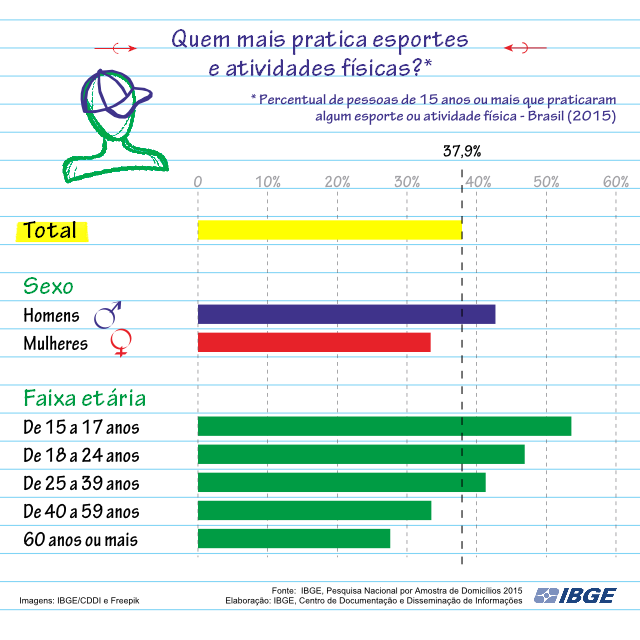
\includegraphics[width=250bp]{PNAD_2015_Esportes_01quem2.png}
\caption{PNAD - Infográfico 1}
\label{est1-fig-2}
\end{figure}

\begin{figure}[H]
\centering
\capstart

\noindent\includegraphics[width=250bp]{{PNAD_2015_Esportes_03instrrend2}.png}
\caption{PNAD - Infográfico 2}
\label{est1-fig-3}
\end{figure}

\begin{figure}[H]
\centering

\includegraphics[width=250bp]{{PNAD_2015_Esportes_04principais}.png}
\caption{PNAD - Infográfico 3}
\label{est1-fig-4}
\end{figure}

\begin{figure}[H]
\centering
\capstart

\noindent\includegraphics[width=250bp]{{PNAD_2015_Esportes_05investimento}.png}
\caption{PNAD - Infográfico 4}
\label{est1-fig-5}
\end{figure}

\begin{enumerate}
\item {} 
Segundo os resultados da pesquisa (veja a \hyperref[est1-fig-2]{figura \ref{est1-fig-2}}), qual a porcentagem de pessoas de 15 anos ou mais que praticaram algum esporte ou atividade física no período de um ano?

\item {} 
O título genérico do infográfico da \hyperref[est1-fig-2]{figura \ref{est1-fig-2}}, a saber, “Quem mais pratica esportes e atividades físicas? - Percentual de pessoas de 15 anos ou mais que praticaram algum esporte ou atividade física-Brasil (2015)”, diz respeito à população brasileira de 15 anos ou mais ou à amostra coletada?

\item {} 
Com base nas recomendações médicas sobre a prática de atividades físicas para se ter boa saúde, como você avalia o resultado obtido na pesquisa para a população brasileira de 15 anos ou mais?

\item {} 
Considerando homens e mulheres separadamente, percebe-se alguma diferença com relação à prática de atividades físicas? Em caso afirmativo, descreva a(s) diferença(s) observada(s).

\item {} 
Considerando as faixas etárias discriminadas no infográfico, percebe-se alguma diferença com relação à prática de atividades físicas? Em caso afirmativo, descreva a(s) diferença(s) observada(s).

\item {} 
Considerando os diferentes graus de instrução (\hyperref[est1-fig-3]{figura \ref{est1-fig-3}}), percebe-se alguma diferença com relação à prática de atividades físicas? Em caso afirmativo, descreva a(s) diferença(s) observada(s).

\item {} 
Considerando as faixas de rendimento mensal per capita do domicílio, percebe-se alguma diferença com relação à prática de atividades físicas? Em caso afirmativo, descreva a(s) diferença(s) observada(s).

\item {} 
Qual foi a variável estudada no gráfico da \hyperref[est1-fig-4]{figura \ref{est1-fig-4}}?

\item {} 
A variável estudada no gráfico da \hyperref[est1-fig-4]{figura \ref{est1-fig-4}} tem respostas de que tipo: numéricas ou não-numéricas?

\item {} 
Qual foi a resposta que apresentou a maior frequência no gráfico da \hyperref[est1-fig-4]{figura \ref{est1-fig-4}}?

\item {} 
O que você acha que representa a resposta “Outros Esportes” no gráfico da \hyperref[est1-fig-4]{figura \ref{est1-fig-4}}?

\item {} 
Qual a porcentagem de pessoas de 15 anos ou mais que concorda com que o poder público deva investir em atividades físicas ou desportivas (\hyperref[est1-fig-5]{figura \ref{est1-fig-5}})?

\item {} 
Qual a opinião das pessoas de 15 anos ou mais que concordam que o poder público deve investir em atividades físicas ou esportivas com relação à prioridade de investimentos?

\item {} 
Entre as pessoas de 15 anos ou mais que não concordam que o poder público deve investir em atividades físicas ou esportivas, que área elas entendem como prioritária?

\item {} 
Podemos afirmar que $57{,}8\%$ das pessoas de 15 anos ou mais defendem que o poder público deve investir em Saúde?"

\end{enumerate}
\end{task}



\arrange{A natureza da estatística}
\label{est1-org-1}

\begin{example}{Opinião dos estudantes sobre lanches na cantina}

Suponha que deseja-se investigar a opinião dos estudantes de um colégio quanto à modificação da lista de produtos vendidos na cantina para outros mais saudáveis, trocando refrigerantes por sucos naturais entre outros. Para isso, a direção da escola irá entrevistar cinco alunos sorteados de cada uma de suas 40 turmas.

\end{example}

\subsection{Conceitos Básicos}
\phantomsection\label{est1-conceitos-1}


Em geral, a palavra população representa um conjunto de habitantes de um determinado lugar. No entanto, em Estatística, \index{população}população tem um sentido mais amplo e pode ser definida como o conjunto de todos os elementos com pelo menos uma característica em comum. Observe que é exatamente essa característica em comum que vai definir o universo (população) de uma pesquisa.

Assim, em Estatística, a população não precisa ser um conjunto de pessoas, pode ser o conjunto de parafusos fabricados por uma indústria, o conjunto de animais de certa espécie que vivem em uma região, todos os estudantes universitários de um país, etc.
\begin{description}
\item[Amostra]\leavevmode\phantomsection\label{est1-def-4} É um subconjunto não-vazio da população.
\end{description}

Cada uma das unidades investigadas em um estudo estatístico é denominada um elemento.  Assim, cada parafuso investigado é um elemento na atividade "Escolha do fornecedor"; cada paciente observado é um elemento na atividade "Comparação de medicamentos"; e cada domicílio e seus residentes são elementos na atividade da PNAD.

Cada característica observada de um elemento é uma \index{variável}variável estatística. Assim, a medida do diâmetro do parafuso é uma variável na atividade "Escolha do fornecedor", o tempo de cura da dor de cabeça é uma variável na atividade "Comparação de medicamentos" e, na atividade da PNAD, estão presentes várias variáveis estatísticas de interesse do domicílio e de seus residentes tais como local, número de cômodos, número de residentes; sexo, idade e rendimento dos residentes, etc.

\begin{description}
\item[{Parâmetro\index{Parâmetro|textbf}}] \leavevmode\phantomsection\label{est1-def-5} Característica numérica da população.

\end{description}
\begin{description}
\item[{Estimador\index{Estimador|textbf}}] \leavevmode\phantomsection\label{est1-def-6} Função que produz estimativas de parâmetros usando os dados da amostra.

\end{description}

\begin{example}{Opinião dos estudantes sobre lanches na cantina (2)}
Considere o exemplo inicial. Nesse caso tem-se:

\begin{itemize}
\item população, correspondendo a todos os estudantes do colégio;
\item amostra, correspondendo aos 200 estudantes entrevistados (5 de cada turma);
\item elemento, correspondendo a cada estudante entrevistado
\item variável de interesse, correspondendo à opinião do estudante: “a favor”{} ou “contra”{} à mudança;
\item parâmetro de interesse, correspondendo à proporção dos estudantes desse colégio que são favoráveis à mudança;
\item estimativa do parâmetro de interesse, correspondendo à proporção entre os 200 estudantes entrevistados favoráveis à mudança.
\end{itemize}

Observação: Em um estudo desse tipo também costumam ser registradas outras variáveis tais como sexo, turno, idade, série etc.
\end{example}

As etapas da análise estatística podem ser divididas em duas estruturas básicas: \index{Estatística Descritiva}Estatística Descritiva e \index{Estatística Inferencial}Estatística Inferencial. A primeira corresponde a uma exploração das informações que podem ser retiradas dos dados amostrais de modo a reconhecer estruturas que possibilitem futuramente inferir sobre parâmetros de interesse. A segunda consiste em estabelecer modelos probabilísticos para que se possa fazer afirmações sobre a população com algum nível de confiança. Leia a caixa \textbf{Para Refletir} do início do capítulo para uma explicação.

Em resumo, a Estatística Descritiva é uma espécie de arqueologia dos dados observados e, a Estatística Inferencial, a indução das informações obtidas da amostra para características da população não observada em sua totalidade.

A PNAD faz uso da inferência estatística, pois ela investiga uma amostra de domicílios em algumas cidades brasileiras, mas propõe estimativas para as características da população brasileira.

Quando se realiza um \index{censo}censo - levantamento de dados de toda a população -, não existe a necessidade de fazer uma inferência estatística. No entanto, muitas vezes a realização de um censo é inviável, por várias razões como custo muito alto, tempo muito longo, entre outras.

\phantomsection\label{est1-class-1}
\subsection{Classificação de Variáveis}

A classificação das variáveis estudadas é importante, pois as técnicas e procedimentos estatísticos de análise de dados dependem do tipo de variável investigado. Nesse sentido é importante reconhecer a natureza de cada variável investigada para posterior tratamento da informação obtida. Por exemplo, se estamos estudando a modalidade de atividades físicas praticadas pelos brasileiros de 15 anos ou mais, não faz sentido calcular média, pois  ela não assume valores numéricos.

Existem dois tipos principais de variáveis (qualitativas e quantitativas), que se subdividem, por sua vez, em duas categorias, conforme a \hyperref[est1-fig-6]{figura \ref{est1-fig-6}}.

\begin{figure}[H]
\centering
\begin{tikzpicture}

\tikzstyle{vecArrow} = [thick, decoration={markings , mark=at position
1 with {\arrow[semithick, fill=white]{triangle 60}}},
double distance=1.4pt, shorten >= 5.5pt,
preaction = {decorate,line width=1.4pt},
postaction = {draw,line width=1.4pt, white,shorten >= 4.5pt}]

\begin{scope}[x=15, y=10]

   \draw[rounded corners = 5pt, fill=\currentcolor!80] (-9,0) rectangle (-5,2);
   \node[font=\bfseries, color=white] at (-7,1) {nominal};
   \draw[rounded corners = 5pt, fill=\currentcolor!80] (-4.5,0) rectangle (-0.5,2);
   \node[font=\bfseries, color=white] at (-2.5,1) {ordinal};
   \draw[rounded corners = 5pt, fill=\currentcolor!80] (0.5,0) rectangle (4.5,2);
   \node[font=\bfseries, color=white] at (2.5,1) {discreta};
   \draw[rounded corners = 5pt, fill=\currentcolor!80] (5,0) rectangle (9,2);
   \node[font=\bfseries, color=white] at (7,1) {contí­nua};
   \draw[vecArrow] (-4.75,3.25) -- (-6,1.5);
   \draw[vecArrow] (-4.75,3.25) -- (-3.5,1.5);
   \draw[vecArrow] (4.75,3.25) -- (6,1.5);
   \draw[vecArrow] (4.75,3.25) -- (3.5,1.5);
   \draw[rounded corners = 5pt, fill=\currentcolor!80] (-9,3) rectangle (-0.5,5);
   \node[font=\bfseries, color=white] at (-4.75,4) {qualitativa};
   \draw[rounded corners = 5pt, fill=\currentcolor!80] (0.5,3) rectangle (9,5);
   \node[font=\bfseries, color=white] at (4.75,4) {quantitativa};
   \draw[vecArrow] (0,6.25) -- (-1.5,4.5);
   \draw[vecArrow] (0,6.25) -- (1.5,4.5);
   \draw[rounded corners = 5pt, fill=\currentcolor!80] (-9,6) rectangle (9,8);
   \node[font=\bfseries, color=white] at (0,7) {Variável};


\end{scope}
\end{tikzpicture}
\caption{Classificação dos tipos de variáveis}
\label{est1-fig-6}
\end{figure}

\begin{description}
\item[{Variável qualitativa\index{Variável qualitativa|textbf}}] \leavevmode\phantomsection\label{est1-def-7}
Uma variável estatística é qualitativa se as possíveis respostas para ela são atributos não-numéricos. A maior parte das variáveis identificadas no "Suplemento de Práticas de Esporte e Atividade Física" da PNAD/2015, representa variáveis qualitativas.
\end{description}

É comum encontrar o termo \textbf{variável categórica} para se referir a uma variável qualitativa. As variáveis qualitativas são classificadas como nominal ou ordinal.

\begin{description}
\item[{Variável qualitativa nominal\index{Variável qualitativa nominal|textbf}}] \leavevmode\phantomsection\label{est1-def-8}
Uma variável qualitativa é nominal quando não existe nenhuma ordenação natural das respostas associadas à variável. Exemplos de variáveis nominais: bairro de residência, tipo sanguíneo, modalidade de atividade física que pratica, etc.
\end{description}

\begin{description}
\item[{Variável qualitativa ordinal\index{Variável qualitativa ordinal|textbf}}] \leavevmode\phantomsection\label{est1-def-9}
A variável qualitativa é ordinal quando é possível estabelecer uma relação de ordem entre as respostas associadas a ela. Por exemplo, nível de instrução da mãe com as respostas possíveis: Ensino Fundamental completo, Ensino Médio completo, Ensino Superior incompleto e Ensino Superior completo. Podemos perceber que quem tem Ensino Médio completo tem maior nível de instrução de quem tem Ensino Fundamental completo.
\end{description}

\begin{description}
\item[{Variável quantitativa\index{Variável quantitativa|textbf}}] \leavevmode\phantomsection\label{est1-def-10}
Uma variável é quantitativa se as respostas para ela são numéricas. Exemplos de variáveis quantitativas são idade, peso, altura, temperatura, número de irmãos, número de horas semanais dedicadas à prática de atividade física.
\end{description}

Uma variável quantitativa é classificada em discreta ou contínua.

\begin{description}
\item[{Variável quantitativa discreta\index{Variável quantitativa discreta|textbf}}] \leavevmode\phantomsection\label{est1-def-11}
As variáveis discretas resultam de uma contagem ou são variáveis cuja quantidade de valores possíveis é finita. Por exemplo, o número de atendimentos em um Pronto-Socorro nos finais de semana, o número de erros de impressão na página de um livro, número de irmãos, etc.

\end{description}
\begin{description}
\item[{Variável quantitativa contínua\index{Variável quantitativa contínua|textbf}}] \leavevmode\phantomsection\label{est1-def-12}
As variáveis quantitativas contínuas em geral resultam de uma medição. Por exemplo, altura, peso, temperatura, etc.
\end{description}


\begin{observation}{}
Na análise dos infográficos vimos que uma variável quantitativa pode ser tratada como qualitativa, por exemplo, a idade trabalhada em faixas etárias torna-se uma variável qualitativa ordinal. No entanto, se consideramos a idade em anos completos temos uma variável quantitativa. Por outro lado, também podemos transformar uma variável qualitativa em quantitativa. Considere a variável “prática de atividades físicas”{} que tem como respostas “Sim”{} ou “Não”. Esse tipo de variável com apenas duas respostas é chamado variável binária e tem uma representação numérica natural. Podemos atribuir o número 1 para a resposta “Sim”{} e o número 0 para a resposta “Não”{}. Essa estratégia permite somar todas as respostas. Observe que a soma representará o número de pessoas na amostra que praticam atividade física e a “média”{} representará a proporção de pessoas na amostra que praticam atividade física. Lembre-se o tratamento dos dados está diretamente relacionado a sua classificação. Os gráficos para representar distribuições de frequências de dados são vinculados ao tipo de dado. Para dados qualitativos, usa-se em geral os gráficos de barras e os gráficos de setores. Para dados quantitativos, usa-se em geral histogramas, ramo-e-folhas e boxplots.
\end{observation}

\subsection{Tabelas de frequências e gráficos para variáveis qualitativas}

\begin{example}{Frequência absoluta e frequência relativa}

Numa turma de um colégio foram observados os tipos sanguíneos de seus 40 alunos. Verificou-se que 18 alunos têm sangue tipo "O", 12, tipo "A", 6, tipo "AB"{} e 4, tipo "B". Nesse exemplo, temos que as \index{frequência absoluta}frequências absolutas para os tipos sanguíneos "O", "A", "AB"{} e "B" foram, respectivamente, 18, 12, 6 e 4. Em geral, quando queremos comparar grupos diferentes, usamos a \index{frequência relativa}frequência relativa em vez da frequência absoluta. A frequência relativa é dada pela razão entre a frequência absoluta e o número total de observações. Nesse exemplo, temos que as frequências relativas para os tipos sanguíneos "O", "A", "AB"{} e "B"{} foram, respectivamente, $0{,}45$; $0{,}30$; $0{,}15$ e $0{,}10$. Observe que em termos percentuais as frequências relativas observadas equivalem a, respectivamente, $45\%$, $30\%$, $15\%$ e $10\%$.

É comum resumir esse tipo de informação, usando uma tabela, informando as respostas da variável e suas frequências. Nesse exemplo a variável é tipo sanguíneo e sua classificação é qualitativa nominal, pois assume respostas não numéricas "A", "B", "AB"{} e "O", sem uma ordenação natural. Em geral dispomos os valores dessa variável em ordem decrescente de frequência.


\centering \setlength\tabcolsep{2.5pt}
\begin{table}[H]
\centering
\begin{tabu} to \linewidth{|c|c|c|c|}
\hline
\thead
tipo sanguíneo  & frequência absoluta  & frequência relativa  &  porcentagem (\%) \\
\hline
O & 18 & $0{,}45$ & $45$ \\
\hline
A & 12 & $0{,}30$ & $30$ \\
\hline
AB & 6 & $0{,}15$ & $15$ \\
\hline
B & 4 & $0{,}10$ & $10$ \\
\hline
total & 0 & $1{,}00$ & $100$ \\
\hline
\end{tabu}
\end{table}

A \textbf{frequência absoluta} de cada resposta da variável qualitativa representa o número de observações dessa resposta. Assim, para a variável tipo sanguíneo e o conjunto de alunos dessa turma, as frequências absolutas dos tipos “O”, “A”, “AB”{} e “B”{} são, respectivamente, 18, 12, 6 e 4. Ou seja, ao todo observaram-se 18 alunos com sangue tipo “O”, 12 alunos com sangue tipo “A”, 6 alunos com sangue tipo “AB”{} e 4 alunos com sangue tipo “B”.

A \textbf{frequência relativa} de cada resposta da variável qualitativa representa o quociente da frequência absoluta da resposta sobre o número total de observações. Observe que a frequência relativa sempre será um número entre $0$ e $1$ e que a soma das frequências relativas será sempre igual a $1$. Veja na tabela desse exemplo.

Uma forma equivalente à frequência relativa é a porcentagem de cada resposta que é dada pelo produto da frequência relativa por $100$. Veja na tabela desse exemplo.
\end{example}

Nas análises dos infográficos, trabalhamos com alguns tipos de gráficos para representar a distribuição de frequências de variáveis qualitativas. No \hyperref[est1-fig-4]{infográfico 3 (Figura \ref{est1-fig-4}}), tem-se um gráfico de barras. Nesse gráfico, cada barra, de mesma largura, representa uma resposta e seu comprimento corresponde à frequência na qual a resposta ocorreu. Observe também que, nesse gráfico, se estivermos trabalhando com as porcentagens de cada resposta, a soma das porcentagens deve ser $100\%$.

Em geral, se a variável qualitativa for ordinal dispomos as respostas em ordem crescente, considerando as respostas. Se a variável é nominal, podemos dispor as respostas em ordem decrescente de frequência.

Alguns gráficos apresentados na atividade “Análise de infográficos” como o \hyperref[est1-fig-4]{infográfico 1 (Figura \ref{est1-fig-2}}) e \hyperref[est1-fig-4]{infográfico 2 (Figura \ref{est1-fig-2}}) usam barras para representar as frequências em subgrupos diferentes do conjunto observado. Mas eles não se encaixam na apresentação anterior. Verifique que se somarmos as porcentagens elas não resultarão em $100\%$. De fato, são gráficos de barras múltiplas, úteis para comparar distribuições de frequências em subgrupos distintos. Observe que, em cada um desses gráficos, a variável sob investigação é se a pessoa pratica ou não atividade física. No entanto, em vez de apresentar as porcentagens das respostas \textit{Sim} e \textit{Não} no subgrupo considerado, como a variável é binária, só foram apresentadas as porcentagens de Sim em cada subgrupo, pois nesse caso, as correspondentes porcentagens de Não são dadas pelo complementar em cada subgrupo considerado. Observe que os subgrupos comparados foram:

\begin{itemize}
\item homens e mulheres;
\item faixas etárias: 15 a 17; 18 a 24; 25 a 39; 40 a 59 e 60 anos ou mais;
\item graus de instrução: sem instrução; fundamental incompleto; fundamental completo; médio incompleto; médio completo; superior incompleto e superior completo;
\item rendimento: menos de 1/2; de 1/2 a 1; de 1 a 2; de 2 a 3; de 3 a 5 e 5 salários mínimos ou mais.
\end{itemize}

Na \hyperref[est1-fig-7]{figura \ref{est1-fig-7}} foi realçado o caso dos subgrupos homens e mulheres da pesquisa.

\begin{figure}[H]
\centering
\capstart

\noindent
\includegraphics[width=400pt]{{barrasmultiplas_sexo}.png}
\caption{Detalhe legendado do \hyperref[est1-fig-2]{infografico 2}}
\label{est1-fig-7}
\end{figure}

O mesmo ocorre quando analisamos os gráficos para faixa etária, grau de instrução e rendimento. Todos são gráficos de barras múltiplas que nos apoiaram em nossas análises sobre a associação entre a prática de atividades físicas e a outra variável (sexo, faixa etária, grau de instrução, rendimento).

No {\hyperref[est1-fig-5]{infográfico 4 (Figura \ref{est1-fig-5})}, temos um gráfico de setores e dois gráficos de retângulos. A ideia por trás desses gráficos é subdividir de maneira proporcional a figura maior em partes cujas áreas em relação à figura maior correspondam à frequência de cada resposta.

No gráfico de setores, subdividimos o círculo em setores circulares de tal modo que o quociente da área de cada setor em relação a área do círculo é igual à frequência relativa (ou porcentagem) da resposta que ele representa. Lembrando que o setor circular é definido pelo ângulo central, para traçar os setores em um gráfico desse tipo será necessário calcular as medidas dos ângulos centrais dos setores correspondentes a cada resposta da variável qualitativa.


Por exemplo, se numa distribuição a frequência relativa de uma resposta corresponde a $0{,}40$ ($40\%$) de todo o conjunto observado, no gráfico de setores essa resposta será representada por um setor circular cujo ângulo central é dado por $0{,}4\times360^{\circ}=144^{\circ}$ como ilustra a \hyperref[setor]{figura \ref{setor}}.

\begin{figure}[H]
\centering

\begin{tikzpicture} [scale=3]
\draw [thick] circle (1);

\clip circle (1);
\draw [very thick] (0,0) -- (0:2) -- (-72:3) -- (-144:2) -- cycle;
\clip (0,0) -- (0:2) -- (-72:3) -- (-144:2);
\fill [\currentcolor!80] circle (1);
\draw circle (.1);
\node at (-72:.2) {$144^{\circ}$};
\end{tikzpicture}
\caption{Setor circular de $144^{\circ}$}
\label{setor}
\end{figure}

A medida da área da região em azul no círculo da \hyperref[setor]{figura \ref{setor}} corresponde à $40\%$ da área do círculo.

Nos gráficos de retângulos essa mesma ideia é usada: o retângulo maior é subdividido em retângulos cujas áreas relativas correspondem às porcentagens das respostas que eles representam. Esses gráficos foram construídos para representar as respostas à pergunta “Em quais áreas em que deve ocorrer investimento público?”{} para quem respondeu \textit{Não} à pergunta “O poder público deve investir em atividades físicas ou desportivas?”{} e também para representar as respostas à pergunta “Qual deve ser a prioridade nos investimentos?” para quem respondeu “Sim”{} à pergunta “O poder público deve investir em atividades físicas ou desportivas?”.

\begin{example}{Frequência absoluta ou frequência relativa?}
Suponha o exemplo com os dados de tipos sanguíneos dos 40 alunos de uma turma. Agora desejamos comparar as respostas obtidas com um conjunto de 120 observações para as quais 30 são tipo A, 12, do tipo AB, 18, do tipo B 60, do tipo O. Os gráficos de barras na mesma escala, usando a frequência absoluta parecem bem diferentes, como mostra a figura a seguir.

\begin{figure}[H]
\centering
Distribuições de frequências de tipo sanguíneo
\vspace{2em}

\begin{tikzpicture}[scale=.14]

  \draw (0,0) -- (0,60);
  \foreach \x in {0,10,...,60}
  {
    \draw [overlay] (0,\x) -- (-.75,\x);
    \node [left, overlay] at (-.75,\x) {\x};
  };

  \foreach \x/\y in {12/0,6/7.5,4/15,18/22.5}
  {
    \draw [fill=\currentcolor!80] (\y+1,0) rectangle (\y+7.5,\x);
  };

\foreach \x/\y in {3.75/A,7.5+3.75/AB,15+3.75/B,22.5+3.75/O} \node at (\x+.1,-2) {\y};

\node [below] at (15,-5) {(40 observações)};
\node [above, rotate=90] at (-5,30) {porcentagem};
\end{tikzpicture}\hspace{1em}
\begin{tikzpicture}[scale=.14]

  \draw (0,0) -- (0,60);
  \foreach \x in {0,10,...,60}
  {
    \draw [overlay] (0,\x) -- (-.75,\x);
    \node [left, overlay] at (-.75,\x) {\x};
  };

  \foreach \x/\y in {30/0,12/7.5,18/15,60/22.5}
  {
    \draw [fill=\currentcolor!80] (\y+1,0) rectangle (\y+7.5,\x);
  };

\foreach \x/\y in {3.75/A,7.5+3.75/AB,15+3.75/B,22.5+3.75/O} \node at (\x+.1,-2) {\y};

\node [below] at (15,-5) {(120 observações)};
\node [above, rotate=90] at (-5,30) {porcentagem};
\end{tikzpicture}

\caption{Gráficos de barras da distribuição na escala da frequência absoluta}
\label{sangue1}
\end{figure}

Porém, os gráficos construídos, usando a escala da porcentagem, não parecem tão diferentes, como mostra a figura a seguir.

\begin{figure}[H]
\centering
Distribuições de frequências de tipo sanguíneo
\vspace{2em}

\begin{tikzpicture}[scale=.14]

  \draw (0,0) -- (0,50);
  \foreach \x in {0,10,...,50}
  {
    \draw [overlay] (0,\x) -- (-.75,\x);
    \node [left, overlay] at (-.75,\x) {\x};
  };

  \foreach \x/\y in {30/0,15/7.5,10/15,45/22.5}
  {
    \draw [fill=\currentcolor!80] (\y+1,0) rectangle (\y+7.5,\x);
  };

\foreach \x/\y in {3.75/A,7.5+3.75/AB,15+3.75/B,22.5+3.75/O} \node at (\x+.1,-2) {\y};

\node [below] at (15,-5) {(40 observações)};
\node [above, rotate=90] at (-5,30) {frequência absoluta};
\end{tikzpicture}\hspace{1em}
\begin{tikzpicture}[scale=.14]

  \draw (0,0) -- (0,50);
  \foreach \x in {0,10,...,50}
  {
    \draw [overlay] (0,\x) -- (-.75,\x);
    \node [left, overlay] at (-.75,\x) {\x};
  };

  \foreach \x/\y in {25/0,10/7.5,15/15,50/22.5}
  {
    \draw [fill=\currentcolor!80] (\y+1,0) rectangle (\y+7.5,\x);
  };

\foreach \x/\y in {3.75/A,7.5+3.75/AB,15+3.75/B,22.5+3.75/O} \node at (\x+.1,-2) {\y};

\node [below] at (15,-5) {(120 observações)};
\node [above, rotate=90] at (-5,30) {frequência absoluta};
\end{tikzpicture}

\caption{Gráficos de barras na escala da porcentagem}
\label{sangue2}
\end{figure}


Comparando os dois, percebem-se apenas pequenas diferenças quanto às porcentagens dos sangues tipo “AB”{} e tipo “B”, comparando os dois gráficos.

\end{example}

Quando estamos trabalhando com variáveis qualitativas usamos a escala da frequência (absoluta, relativa ou porcentagem de cada resposta) na construção de gráficos para representar a distribuição de frequências das respostas dadas à variável sob investigação. As representações gráficas mais comuns são gráficos de barras ou colunas e gráficos de setores. Para comparações da mesma variável em grupos diferentes é comum usar o gráfico de barras múltiplas com frequências relativas ou porcentagens.

\begin{observation}{}

Como escolher entre o gráfico de setores ou o gráfico de barras para representar a distribuição de frequências de uma variável qualitativa?

Se o número de respostas diferentes é grande, maior que 4, ou se as diferenças nas frequências das respostas são pequenas, por exemplo uma tem porcentagem $22\%$ e a outra tem porcentagem $25\%$, o gráfico de setores não será adequado, pois pequenas diferenças de ângulos não são perceptíveis, enquanto que com o gráfico de barras é fácil perceber pequenas diferenças.

Também, quando deseja-se fazer comparações múltiplas o gráfico de setores não é adequado. Observe que todos infográficos da atividade “Análise de infográficos”{} para comparar diferentes grupos quanto à prática de atividades físicas são gráficos de barras múltiplas.

\end{observation}

\clearpage
\def\currentcolor{session2} 
\begin{objectives}{Prática de atividade física na turma}
{
\begin{itemize}
\item Conduzir uma coleta de dados sobre a turma envolvendo as informações do suplemento “Prática de Esporte e Atividade Física” para comparar os resultados dessa “amostra” com os da PNAD/2015.

\end{itemize}
}{1}{2}
\end{objectives}
\marginpar{\vspace{-2em}}
\begin{sugestions}{Prática de atividade física na turma}
{
\begin{itemize}
\item Preparar uma tabela a ser preenchida pela turma com as informações: sexo, idade, prática ou não de atividade física em seu tempo livre, e a modalidade, de maneira a viabilizar a comparação dos dados obtidos com os resultados da PNAD/2015. A tabela poderá conter outras variáveis se forem julgadas de interesse pela turma como por exemplo, local da prática, duração da prática entre outras. Mas, para efeito de comparação com os infográficos, sexo e idade serão as variáveis necessárias nesse levantamento. Comente com os alunos que essa será uma amostra de conveniência, pois o interesse é estudar o perfil da turma quanto à prática de atividades físicas e por isso, as respostas da turma podem não ser similares às da pesquisa.

\item Com base nas respostas obtidas, resumir a informação em tabelas de frequências, contar quantas respostas foram sim, calcular a porcentagem da turma que pratica atividade física e comparar com o resultado geral das pessoas de 15 anos ou mais, o percentual correspondente a essa faixa etária e o percentual correspondente a esse grau de instrução. Construir uma tabela de frequências com as modalidades esportivas incluindo as categorias apresentadas no infográfico do IBGE. Construir gráficos para representar as distribuições de frequências das variáveis investigadas nessa pesquisa. Construir gráficos de barras múltiplas, isto é, gráficos de barras separados por grupos diferentes, como por exemplo, sexo.
\end{itemize}
}{1}{2}
\end{sugestions}
\marginpar{\vspace{-2em}}
\begin{objectives}{Classificação de variáveis}
{
\begin{itemize}
\item Diferenciar variável qualitativa e variável quantitativa.
\item Identificar variáveis qualitativas binárias.
\end{itemize}
}{1}{2}
\end{objectives}
\begin{answer}{Classificação de variáveis}
{
\begin{enumerate}
 \begin{multicols}{3}
  
 \item quantitativa.
 \item quantitativa.
 \item quantitativa.
 \item quantitativa. 
 \item qualitativa binária.
 \item qualitativa.
 \item quantitativa. 
 \item quantitativa.
 \item qualitativa binária.
 \item quantitativa.
 \item qualitativa binária.
 \item qualitativa.
 \end{multicols}
\end{enumerate}
}{0}
\end{answer}
\clearmargin
\begin{objectives}{Construção de gráficos para variáveis qualitativas}
{
\begin{itemize}
\item Construir gráficos de distribuições de frequências para variáveis qualitativas.
\end{itemize}
}{1}{1}
\end{objectives}
\begin{sugestions}{Construção de gráficos para variáveis qualitativas}
{
Embora os gráficos solicitados nesta atividade sejam simples, recomenda-se sugerir aos alunos usar algum recurso tecnológico para a construção dos mesmos, tais como, uma planilha ou o GeoGebra.
}{1}{1}
\end{sugestions}
\begin{answer}{Construção de gráficos para variáveis qualitativas}
{
\begin{figure}[H]
\centering

\begin{tikzpicture}
\begin{scope}[x=19,y=19, scale=.75]
\node at (0,11) {O poder público deve investir em atividades fí­sicas?};
\draw [fill=session2!80] (-1,10) rectangle (1,2.67);
\draw [fill=session3!80] (-1,2.67) rectangle (1,1.2);
\draw [fill=secundario!80] (-1,1.2) rectangle (1,0);
\node [color=white] at (0,6.335) {\textbf{Sim}};
\node [color=white] at (0,1.935) {\textbf{Não}};
\draw [thick,->] (-1.5,9.5) -- (-7,9.5) -- (-7,8.5); 
\draw [thick,->] (1.5,1.935) -- (7,1.935) -- (7,3); 
\draw[fill=session2!80] (7,7) -- (7,10) arc (90:-118.08:3);
\draw [fill=primario!80] (7,7) -- + (-118.08:3) arc (-118.08:-194.76:3);
\draw [fill=session1!80] (7,7) -- + (-194.76:3) arc (-194.76:-254.16:3);
\draw [fill=secundario!80] (7,7) -- + (-254.16:3) arc (-254.16:-270:3);
\draw (7,7) -- (7,10);
\draw[fill=session4!80] (-7,4.5) -- (-7,7.5) arc (90:-237.96:3);
\draw [fill=box3!80] (-7,4.5) -- + (-237.96:3) arc (-237.96:-266.76:3);
\draw [fill=secundario!80] (-7,4.5) -- + (-266.76:3) arc (-266.76:-270:3);
\draw (-7,4.5) -- (-7,7.5);
\draw [fill=session4!80, line width=0] (-10,-1) rectangle (-9,-2);
\node [right] at (-9,-1.5) {Atividades para};
\node [right] at (-9,-2.5) {pessoas em geral};
\draw [fill=box3!80, line width=0] (-10,-3.5) rectangle (-9,-4.5);
\node [right] at (-9,-4) {Formação de atletas};
\draw [fill=secundario!80, line width=0] (-10,-5) rectangle (-9,-6);
\node [right] at (-9,-5.5) {Outra};
\draw [fill=session1!80, line width=0] (4,-1) rectangle (5,-2);
\node [right] at (5,-1.5) {Saúde};
\draw [fill=primario!80, line width=0] (4,-2.5) rectangle (5,-3.5);
\node [right] at (5,-3) {Segurança};
\draw [fill=session2!80, line width=0] (4,-4) rectangle (5,-5);
\node [right] at (5,-4.5) {Educação};
\draw [fill=secundario!80, line width=0] (4,-5.5) rectangle (5,-6.5);
\node [right] at (5,-6) {Outra};
\end{scope}
\end{tikzpicture}
\end{figure}
}{0}
\end{answer}
\begin{objectives}{Análise de gráfico}
{
\begin{itemize}
\item Mostrar que podem existir diversas formas de usar barras para representar algum tipo de dado, mas que nem todos os gráficos que usam barras são gráficos de barras no sentido da representação de uma distribuição de frequências.
\end{itemize}
}{1}{1}
\end{objectives}
\begin{sugestions}{Análise de gráfico}
{
O gráfico desse exemplo é “um gráfico de barras”, mas as barras representam o valor da inflação da alimentação acumulado nos últimos 12 meses em função do tempo: de agosto de 2016 até agosto de 2017. Na seção “Explorando 2”, veremos que, para esse tipo de informação - valores de uma variável quantitativa ao longo do tempo -, é mais comum usar um gráfico de linhas unindo por segmentos os pontos consecutivos dados (tempo, valor da variável).
}{1}{1}
\end{sugestions}
\begin{answer}{Análise de gráfico}
{
\begin{enumerate}
\item É um gráfico que usa barras, mas nesse gráfico o comprimento das barras não é frequência.

\item Valor da inflação da alimentação acumulada nos últimos 12 meses. Esses valores são apresentados em função do período de tempo: agosto de 2016 até agosto de 2017.

\item O valor da inflação da alimentação acumulada nos últimos 12 meses é uma variável quantitativa, o período de tempo representado em mês/ano é uma variável qualitativa ordinal.

\item (gráfico) Como evoluiu a inflação da alimentação acumulada em 12 meses no período investigado, a saber, agosto de 2016 até agosto de 2017. Mais precisamente, percebe-se que a inflação da alimentação acumulada em 12 meses apresentou no período analisado uma forte tendência de queda.

\begin{figure}[H]
\centering


\begin{tikzpicture}
\begin{scope}[x=20, y=10, scale=.7]
      \draw (0,0) -- (28,0);
      \draw (0,-7) -- (0,20);

      \foreach \ye in {-5,0,5,10,15,20}{
         \draw [help lines, gray] (0,\ye) -- (28,\ye);
         \node [left, overlay] at (0,\ye) {\ye};
      };
      \foreach \x/\y/\z in {1/16.79/AGO,2/16.11/SET,3/14.85/OUT,4/11.57/NOV,5/9.36/DEZ,6/6.47/JAN,7/4.34/FEV,8/3/MAR,9/2.54/ABR,10/1.08/MAI,11/-0.56/JUN,12/-3.07/JUL,13/-5.19/AGO}{
      \draw [help lines, gray] (2*\x,-7) -- (2*\x,20);
      \node at (2*\x,-8) {\z};
      }
    \draw [help lines] (2*14,-7) -- (2*14,20);
      \draw [color=primario, very thick] (2,16.79) node[ponto] {}
      \foreach \x/\y/\z in {1/16.79/AGO,2/16.11/SET,3/14.85/OUT,4/11.57/NOV,5/9.36/DEZ,6/6.47/JAN,7/4.34/FEV,8/3/MAR,9/2.54/ABR,10/1.08/MAI,11/-0.56/JUN,12/-3.07/JUL,13/-5.19/AGO}{
         -- (2*\x,\y) node[ponto] {}
      };
      \node at (2,-9.5) {2016};
      \node at (12,-9.5) {2017};
      \node [right] at (0,23.5) {INFLAÇÃO DA ALIMENTAÇÃOO NO DOMICÍLIO};
      \node [right] at (0,22) {(acumulado em 12 meses, em $\%$)};
      \end{scope}
\end{tikzpicture}
\end{figure}
\end{enumerate}
}{9}
\end{answer}


\practice{A natureza da estatística}
\label{est1-prac-1}


\phantomsection\label{est1-ativ-5}
\begin{task}{ Prática de atividade física na turma}

Deseja-se comparar os hábitos de atividade física em tempo livre dos alunos da turma com os dados obtidos da PNAD/2015. Para isso preencha o formulário de dados fornecido pelo professor. Construa tabelas e gráficos resumindo a informação obtida.
\end{task}
\phantomsection\label{est1-ativ-6}
\begin{task}{ Classificação de variáveis}

Suponha que cada uma das variáveis a seguir foi observada para todos os alunos de sua turma. Indique se cada uma delas é uma variável qualitativa ou quantitativa. Se for uma variável qualitativa, indique se ela é binária (apenas duas respostas possíveis) ou não.
\begin{enumerate}
\item {} 
Altura (em metros).

\item {} 
Peso (em quilos).

\item {} 
Índice de massa corporal (IMC) dado pelo quaociente entre o peso (em quilos) e o quadrado da medida da altura (em metros).

\item {} 
Tempo de sono na noite anterior.

\item {} 
Se foi dormir na noite anterior antes ou depois da meia-noite.

\item {} 
Mês de nascimento.

\item {} 
Número de irmãos.

\item {} 
Nota obtida na última avaliação de Matemática.

\item {} 
Se tirou nota maior ou igual a 6,0 ou menor do que 6,0 na última avaliação de Matemática.

\item {} 
Distância da casa à escola.

\item {} 
Se o indivíduo possui cartão de crédito ou não.

\item {} 
Modo de locomoção para a escola.

\end{enumerate}
\end{task}
\clearpage
\phantomsection\label{est1-ativ-7}

\begin{task}{ Construção de gráficos para variáveis qualitativas}

Considerando o \hyperref[est1-fig-5]{infográfico 4}, transforme o gráfico de setores em gráfico de retângulos e os gráficos de retângulos em gráficos de setores.
\end{task}

\phantomsection\label{est1-ativ-8}
\begin{task}{ Análise de gráfico}

Observe o gráfico a seguir publicado em um jornal.

\begin{figure}[H]
\centering
\begin{tikzpicture}[scale=0.7, every node/.style={scale=0.9}]
\begin{scope}[x=20, y = 10]
\draw (0,0) -- (28,0);
\foreach \ye in {-5,5,10,15}{
\draw [help lines, lightgray] (0,\ye) -- (28,\ye);
}
\foreach \x/ \y/\z in {1/16.79/AGO,2/16.11/SET,3/14.85/OUT,4 /11.57/NOV,5/9.36/DEZ,6/6.47/JAN,7/4.34/FEV,8/3/MAR,9 /2.54/ABR,10/1.08/MAI,11/-0.56/JUN,12/-3.07/JUL,13/-5.19 /AGO}{
   \draw [fill=\currentcolor!80] (2*\x-0.5,0) rectangle  (2*\x+0.5,\y);
   \node at (2*\x,-8) {\z};
}

\foreach \x/\y/\z in {1/16/79,2/16/11,3/14/85,4/11/57,5/9/36,6/6/47,7/4/34,8/3/0,9/2/52,10/1/08} 
\node [above] at (2*\x,\y.\z) {\y,\z};

\foreach \x/\y/\z in {11/-0/56,12/-3/07,13/-5/19} 
\node [below] at (2*\x,\y.\z) {\y,\z};

\node at (2,-10) {2016};
\node at (12,-10) {2017};
\node [right] at (0,21.5) {INFLAÇÃO DA ALIMENTAÇÃO NO   DOMICÍLIO};
\node [right] at (0,20) {(acumulado em 12 meses, em   $\%$)};
\end{scope}
\end{tikzpicture}
\caption{Inflação da alimentação acumulada nos últimos 12 meses (Fonte: IBGE)}
\label{est1-fig-8}
\end{figure}

\begin{enumerate}
\item {} 
Como você classificaria esse gráfico?

\item {} 
Qual é a informação representada pelo comprimento da barra nesse gráfico?

\item {} 
Que tipo(s) de variável(is) ele está representando?

\item {} 
Construa um gráfico diferente para representar a mesma informação, marcando num plano Cartesiano os pontos $(x,y)$ em que $x$ corresponde ao tempo e $y$ corresponde à inflação acumulada no domicílio, unindo os pontos consecutivos por segmentos. É possível perceber a partir desse gráfico algum tipo de comportamento no período observado?

\end{enumerate}


\end{task}

\cleardoublepage
\def\currentcolor{session1}
\begin{objectives}{Construção do histograma}
{
\begin{itemize}
\item Identificar, na construção de um gráfico que represente a distribuição de frequências, a necessidade de agrupar em intervalos de classe os valores observados de uma variável quantitativa contínua.
\end{itemize}
}{1}{1}
\end{objectives}
\begin{sugestions}{Construção do histograma}
{
A construção do histograma será dirigida nessa atividade, mas recomenda-se fortemente o uso de recursos tecnológicos, como o GeoGebra, para esse tipo de construção.

Incluir link do arquivo desses dados em formato GeoGebra. Em alguns aplicativos, e é o caso do GeoGebra, é necessário substituir a vírgula como separador decimal do padrão brasileiro por ponto.
}{1}{1}
\end{sugestions}
\clearmargin
\marginpar{\vspace{.5em}}
\begin{answer}{Construção do histograma}
{
\begin{enumerate}

\item \adjustbox{valign=t}
{
  \begin{tabu} to \linewidth {|c|c|}
  \hline
  \thead 
  Intervalo de classe & Número de observações \\
  \hline
  ${[} 3{,}0 ; 3{,}5 {[}$ & 2 \\ 
  \hline
  ${[} 3{,}5 ; 4{,}0 {[}$ & 3 \\
  \hline
  ${[} 4{,}0 ; 4{,}5 {[}$ & 7 \\
  \hline
  ${[} 4{,}5 ; 5{,}0 {[}$ & 9 \\
  \hline
  ${[} 5{,}0 ; 5{,}5 {[}$ & 11 \\
  \hline
  ${[} 5{,}5 ; 6{,}0 {[}$ & 11 \\
  \hline
  ${[} 6{,}0 ; 6{,}5 {[}$ & 9 \\
  \hline
  ${[} 6{,}5 ; 7{,}0 {[}$ & 7\\
  \hline
  ${[} 7{,}0 ; 7{,}5 {[}$ & 4 \\
  \hline
  ${[} 7{,}5 ; 8{,}0 {[}$ & 2 \\
  \hline
  \end{tabu}
}
\item[\titem{b)} e \titem{c})]\adjustbox{valign=t}
{
  \begin{tikzpicture} [yscale=0.5, scale=.85]

  \foreach \y in {0,...,12}{
     \draw [help lines,color=secundario!50] (-0.1,\y) -- (12,\y);}

  \foreach \x in {0,12}{
  \draw [help lines, color=secundario!50] (\x,-0.2) -- (\x,12);}

  \foreach \x in {1,...,11}{
  \draw [help lines, color=secundario!50] (\x,0) -- (\x,-0.2);}

  \foreach \y in {0,...,12} \node [left, scale=0.8] at (-0.1,\y) {\y}; 

  \foreach \x/\y/\z in {.5/0/$\leq$ 3.0,1.5/2/3.0 a 2.5,2.5/3/3.5 a 4.0,3.5/7/4.0 a 4.5,4.5/9/4.5 a 5.0,5.5/11/5.0 a 5.5, 6.5/11/5.5 a 6.0, 7.5/9/6.0 a 6.5, 8.5/7/6.5 a 7.0,9.5/3/7.0 a 7.5,10.5/2/7.5 a 8.0,11.5/0/$>$ 8.0} {\node [right, rotate=-90, scale=0.8] at (\x, 0) {\z};

  \draw [fill=\currentcolor!80] (\x-0.5,0) rectangle (\x+0.5,\y);}

  \node [below, rotate=-0, scale=1, align=center] at (6,-1) {$\bigg\uparrow$ \\ Média};
  \end{tikzpicture}
}

\setcounter{enumi}{3}

\item A área do histograma construído é dada por $$A=0{,}5\cdot(2+3+7+9+11+11+9+7+3+2)=0{,}5\cdot64=32.$$

Por exemplo, o quociente da área do primeiro retângulo sobre a área total é $$\displaystyle\frac{0{,}5\cdot2}{32}=\frac{13}{2}=264=0,03125$$ que é a frequência relativa desse intervalo de classe. Da mesma forma, o quociente da área do terceiro retângulo sobre a área total é $$\displaystyle\frac{0{,}5⋅\cdot7}{32}=\frac{3{,}5}{32}=\frac{7}{64}=0{,}109375$$ que é a frequência relativa desse intervalo de classe. Essa verificação ilustra a propriedade do histograma em representar a distribuição de frequências dos dados observados tal que cada retângulo do histograma representa a frequência do intervalo de classe correspondente no conjunto de dados como um todo.
\end{enumerate}
}{1}
\end{answer}
\begin{objectives}{Medição da temperatura ao longo do tempo}
{
\begin{itemize}
\item Definir série temporal a partir de um conjunto de observações sobre uma variável quantitativa contínua variando no tempo.

\item Trabalhar com gráficos de linha para ilustrar a evolução dos valores da variável ao longo do tempo.
\end{itemize}
}{1}{1}
\end{objectives}
\begin{sugestions}{Medição da temperatura ao longo do tempo}
{
Para a construção do gráfico de linha será fornecida uma malha quadriculada para o preenchimento dos pontos, recomenda-se também uso de planilhas de cálculo para essa construção. Veja em \url{shorturl.at/pHJLU} uma sugestão para realizar esta atividade.

Respostas possíveis na reflexão proposta são: índices de inflação, preços de diversos bens, índices da bolsa de valores, a população total em um território, a incidência de alguma enfermidade, a quantidade de vendas de um produto. É importante usar exemplos de dados que tenham aparecido recentemente na mídia ou que tenham relevância local.

Na discussão sobre sazonalidade, pedir aos alunos para trazer notícias de jornais ou revistas que contenham séries temporais. Mostrar que existem várias medições que são comparadas com as do ano anterior, por exemplo, inflação, crescimento do PIB, taxas de desemprego por trimestre, entre outras.
}{1}{1}
\end{sugestions}




\explore{estruturas de variáveis quantitativas}
\label{est1-exp-2}

\phantomsection\label{est1-ativ-9}
\begin{task}{Construção do histograma}

\begin{figure}[H]
\centering
\capstart

\noindent
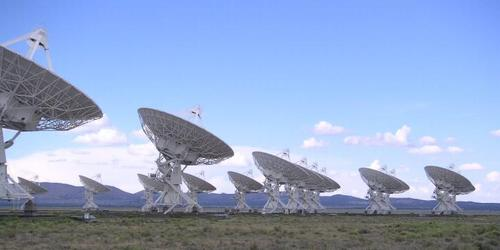
\includegraphics[width=300bp]{USA_NM_VeryLargeArray_03.jpg}

\caption{Arranjo de radiotelescópios - Very Large Array (VLA), New Mexico, EUA. \href{https://commons.wikimedia.org/wiki/File:USA.NM.VeryLargeArray.03.jpg}{Foto: Hajor CC-by-sa}}

\label{est1-fig-9}
\end{figure}

Os radiotelescópios são instrumentos de observação astronômica capazes de captar ondas eletromagnéticas não visíveis a olho nu: as ondas de rádio.

Um arranjo de oito radiotelescópios (A, B, C, D, E, F, G e H) como  ilustrado na \hyperref[est1-fig-9]{Figura \ref{est1-fig-9}} detectou sinais cujos oito registros de tempo para cada radiotelescópio se encontram na tabela a seguir.



\begin{table}[H]
\centering
\begin{tabu} to \linewidth {|c|c|c|c|c|c|c|c|}
\hline
\thead
A & B &  C & D &  E & F &  G &  H \\
\hline
3,03 & 4,37 & 5,04 & 5,73 & 4,03 & 5,37 & 6,04 & 6,74 \\
\hline
3,38 & 4,46 & 5,11 & 5,84 & 4,38 & 5,46 & 6,11 & 6,84 \\
\hline
3,60 & 4,55 & 5,19 & 5,95 & 4,60 & 5,55 & 6,19 & 6,96 \\
\hline
3,78 & 4,63 & 5,29 & 6,08 & 4,78 & 5,64 & 6,29 & 7,08 \\
\hline
3,92 & 4,71 & 5,36 & 6,23 & 4,92 & 5,72 & 6,36 & 7,23 \\
\hline
4,04 & 4,79 & 5,45 & 6,41 & 5,04 & 5,79 & 6,45 & 7,40 \\
\hline
4,16 & 4,87 & 5,54 & 6,62 & 5,16 & 5,87 & 6,54 & 7,63 \\
\hline
4,27 & 4,95 & 5,64 & 6,97 & 5,26 & 5,95 & 6,64 & 7,97 \\
\hline
\end{tabu}
\end{table}

\begin{reflection}
\begin{itemize}
\item {} 
Como construir uma tabela de frequências desses dados uma vez que os registros de tempo são todos distintos?

\item {} 
Como você faria para visualizar o comportamento de uma variável com estas características?

\end{itemize}
\end{reflection}

A natureza quantitativa de uma variável contínua pode muitas vezes levar a resultados que praticamente não se repetem. Eles podem ser todos diferentes, como é observado no exemplo. Com o objetivo de identificar alguma estrutura no comportamento deste tipo de variável é necessário agrupar os valores em intervalos de classe, o que permite analisar a sua distribuição de frequências.

\begin{enumerate}
\item Complete a tabela a seguir que utiliza de intervalos de amplitude $0{,}5$ começando em $3{,}0$. Observe que cada intervalo na tabela é fechado à esquerda e aberto à direita, isto quer dizer que, o limite inferior está incluso e o limite superior não está incluso.

\begin{table}[H]
\centering
\begin{tabu} to \linewidth {|c|c|}
\hline
\thead 
Intervalo de classe & Número de observações \\
\hline
${[} 3{,}0 ; 3{,}5 {[}$ & \\ 
\hline
${[} 3{,}5 ; 4{,}0 {[}$ & \\
\hline
${[} 4{,}0 ; 4{,}5 {[}$ & \\
\hline
${[} 4{,}5 ; 5{,}0 {[}$ & \\
\hline
${[} 5{,}0 ; 5{,}5 {[}$ & \\
\hline
${[} 5{,}5 ; 6{,}0 {[}$ & \\
\hline
${[} 6{,}0 ; 6{,}5 {[}$ & \\
\hline
${[} 6{,}5 ; 7{,}0 {[}$ & \\
\hline
${[} 7{,}0 ; 7{,}5 {[}$ & \\
\hline
${[} 7{,}5 ; 8{,}0 {[}$ & \\
\hline
\end{tabu}
\end{table}

Para visualizar o comportamento desses dados, iremos construir um gráfico chamado \index{histograma}histograma, composto por retângulos adjacentes cujas alturas representam a frequência de observações que ocorrem no intervalo correspondente. A base de cada retângulo corresponde aos limites do intervalo definido no agrupamento dos dados.

\item Complete a figura a seguir com os demais retângulos do \hyperref[est1-fig-10]{histograma}.

\begin{figure}[H]
\centering

\begin{tikzpicture} [yscale=0.5, scale=.85]

\foreach \y in {0,...,12}{
   \draw [help lines,color=secundario!50] (-0.1,\y) -- (12,\y);}

\foreach \x in {0,12}{
\draw [help lines, color=secundario!50] (\x,-0.2) -- (\x,12);}

\foreach \x in {1,...,11}{
\draw [help lines, color=secundario!50] (\x,0) -- (\x,-0.2);}

\foreach \y in {0,...,12} \node [left, scale=0.8] at (-0.1,\y) {\y}; 

\foreach \x/\y in {.5/$\leq$ 3.0,1.5/3.0 a 2.5,2.5/3.5 a 4.0,3.5/4.0 a 4.5,4.5/4.5 a 5.0,5.5/5.0 a 5.5, 6.5/ 5.5 a 6.0, 7.5/6.0 a 6.5, 8.5/6.5 a 7.0,9.5/7.0 a 7.5,10.5/7.5 a 8.0,11.5/$>$ 8.0} \node [right, rotate=-90, scale=.8] at (\x, 0) {\y};

\draw [fill=\currentcolor!80] (1,0) rectangle (2,2);
\end{tikzpicture}
\caption{Histograma dos dados coletados pela grade de radiotelescópios}
\label{est1-fig-10}
\end{figure}

\item Calcule a média dos dados da tabela e localize-a no gráfico, sabendo que a soma dos 64 registros de tempo é $351{,}95$. O que você pode observar quanto à localização da média no histograma construído?

\item Calcule a área correspondente ao histograma construído, somando as áreas dos 10 retângulos do histograma. Verifique que o quociente da área de cada retângulo e da área do histograma é igual à frequência relativa do intervalo de classe que ele representa.

\end{enumerate}
% \begin{figure}[H]
% \centering
% \capstart

% \begin{tikzpicture} [yscale=0.5]

% \foreach \y in {0,...,12}{
%    \draw [help lines,color=secundario!50] (-0.1,\y) -- (12,\y);}

% \foreach \x in {0,12}{
% \draw [help lines, color=secundario!50] (\x,-0.2) -- (\x,12);}

% \foreach \x in {1,...,11}{
% \draw [help lines, color=secundario!50] (\x,0) -- (\x,-0.2);}

% \foreach \y in {0,...,12} \node [left, scale=0.7] at (-0.1,\y) {\y}; 

% \foreach \x/\y/\z in {.5/0/$\leq$ 3.0,1.5/2/3.0 a 2.5,2.5/3/3.5 a 4.0,3.5/7/4.0 a 4.5,4.5/9/4.5 a 5.0,5.5/11/5.0 a 5.5, 6.5/11/5.5 a 6.0, 7.5/9/6.0 a 6.5, 8.5/7/6.5 a 7.0,9.5/3/7.0 a 7.5,10.5/2/7.5 a 8.0,11.5/0/$>$ 8.0} {\node [right, rotate=-90, scale=0.6] at (\x, 0) {\z};

% \draw [fill=\currentcolor!80] (\x-0.5,0) rectangle (\x+0.5,\y);}

% \node [below, rotate=-0, scale=1, align=center] at (6,-.5) {$\bigg\uparrow$ \\ Media};
% \end{tikzpicture}

% \caption{Histograma dos registros de tempo}

% \label{est1-fig-11}

% \end{figure}

\end{task}

\phantomsection\label{est1-ativ-10}
\begin{task}{Medição da temperatura ao longo do tempo}

Você deve ter notado que a previsão do tempo é feita sempre a partir de dois números, isto ocorre porque a temperatura varia de forma contínua ao longo do dia e o que está sendo previsto são as temperaturas máxima e mínima. Por exemplo: 28° / 19°, significa que a previsão da temperatura máxima durante o dia será aproximadamente de 28°C e a mínima 19°C.

Diversas variáveis meteorológicas (no sentido estatístico) são registradas nas estações meteorológicas: temperatura, precipitação (quantidade de chuva), umidade do ar, entre outras.

No Brasil, as estações estão a cargo do \textbf {Instituto Nacional de Meteorologia (INMET)} (\href{http://www.inmet.gov.br}{http://www.inmet.gov.br}) e as informações são armazenadas em bases de dados. Para poder tratar essas informações, frequentemente elas são resumidas por períodos de tempo de diferentes magnitudes: dias, semanas, meses ou anos.

Dados coletados ao longo do tempo (como a informação meteorológica) são conhecidos como séries de dados temporais ou, apenas, \index{séries temporais}séries temporais, já que correspondem a variáveis que mudam continuamente ao longo do tempo e a informação só é útil se sabemos o momento em que foram realizadas as medições.

\begin{reflection}

Forneça outros exemplos de séries temporais nas áreas de saúde, economia, finanças, educação, etc.
\end{reflection}

\justify
A tabela a seguir fornece a média das temperaturas máximas para cada mês nos anos de 1991 a 2000 da cidade de Porto Alegre em graus centígrados (Fonte: \href{http://www.inmet.gov.br/portal/index.php?r=bdmep/bdmep}{Banco de Dados Meteorológicos para Ensino e Pesquisa, BDMEP - INMET})


\begin{table}[H]
\centering
\begin{tabu} to \linewidth {|c|c|c|c|c|c|c|c|c|c|c|}
\hline
\multicolumn{11}{|c|}{\cellcolor{\currentcolor!80}{\textcolor{white}{\textbf{Temperatura Máxima Média mensal nos anos 1991-2000 na cidade de Porto Alegre}}}} \\
\hline
\thead
Mês & 1991 & 1992 & 1993 & 1994  & 1995  & 1996 & 1997 & 1998 & 1999 & 2000 \\
\hline
1 & 30,23 & 30,43 & 31,34 & 30,33 & 30,74 & 29,89 & 32,09 & 29,13 & 30,65 & 30,63 \\
\hline
2 & 31,03 & 31,48 & 29,28 & 28,85 & 29,46 & 29,78 & 29,62 & 28,26 & 29,56 & 29,93 \\
\hline
3 & 30,55 & 30,05 & 28,22 & 28,05 & 29,12 & 28,67 & 28,63 & 27,20 & 31,64 & 27,85 \\
\hline
4 & 26,15 & 25,52 & 27,66 & 25,51 & 26,22 & 27,03 & 26,56 & 24,03 & 24,00 & 26,32 \\
\hline
5 & 25,31 & 21,44 & 23,29 & 24,33 & 21,95 & 22,94 & 22,95 & 22,00 & 21,51 & 21,78 \\
\hline
6 & 20,32 & 22,68 & 19,13 & 20,09 & 20,45 & 17,76 & 19,42 & 19,60 & 18,87 & 21,50 \\
\hline
7 & 19,75 & 16,91 & 17,97 & 20,41 & 21,60 & 16,99 & 20,67 & 20,47 & 18,78 & 17,59 \\
\hline
8 & 21,81 & 20,50 & 21,90 & 21,28 & 21,55 & 22,59 & 23,06 & 19,77 & 21,94 & 20,85 \\
\hline
9 & 23,99 & 22,14 & 20,83 & 25,21 & 22,62 & 21,40 & 22,32 & 21,22 & 22,65 & 22,25 \\
\hline
10 & 26,17 & 26,16 & 26,40 & 24,60 & 24,17 & 25,34 & 23,27 & 25,19 & 23,07 & 24,02 \\
\hline
11 & 26,93 & 27,16 & 28,07 & 26,53 & 28,93 & 28,40 & 26,51 & 28,24 & 26,36 & 26,87 \\
\hline
12 & 30,60 & 29,95 & 29,73 & 32,05 & 30,44 & 29,87 & 30,28 & 28,91 & 29,08 & 29,51 \\
\hline
\end{tabu}
\end{table}
\par

\begin{enumerate}
\item {} 
Escolha dois anos diferentes e localize os pontos da tabela na grade quadriculada usando o mês como abscissa $(x)$ e a temperatura como ordenada $(y)$. Utilize cores diferentes para a série de cada ano.

\item {} 
Una os pontos correspondentes ao mesmo ano (mesma série) de meses consecutivos com um segmento e observe o resultado. Você percebe algum comportamento similar para a  temperatura em anos diferentes?

\item {} 
Compare seu gráfico com o de colegas que escolheram outros anos (ou acrescente séries de outros anos ao seu gráfico). O que você percebe com relação à temperatura nos meses iniciais, intermediários e finais do ano?  A que se deve esse comportamento da temperatura?

\end{enumerate}



\titem{a)} e \titem{b)} Percebe-se temperaturas mais altas nos meses iniciais e finais do ano e, mais baixas, no meio do ano.

\begin{figure}[H]
\centering

\begin{tikzpicture} [yscale=0.5, scale=1.1, every node/.style={scale=1.2}]

\foreach \y in {0,...,10}{
   \draw [help lines,color=secundario!30] (-0.1,\y) -- (11,\y);}

\foreach \x in {0,11}{
\draw [help lines, color=secundario!30] (\x,-0.2) -- (\x,10);}

\foreach \x in {1,...,11}{
\draw [help lines, color=secundario!30] (\x,0) -- (\x,-0.2);}

\node [above, scale=0.8] at (5.5,10) {Temperatura Máxima Média};

\foreach \y/\z in {0/15.0,1/17.0,2/19.0,3/21.0,4/23.0,5/25.0,6/27.0,7/29.0,8/31.0,9/33.0,10/35.0} \node [left, scale=0.6] at (-0.1,\y) {\z}; 

\foreach \x in {1,...,12} \node [below, scale=0.6] at (\x-1,-0.2) {\x};

\foreach \x/\y/\z in {1/1991/destacado,2/1992/green!50!black,3/1993/atento,4/1994/cyan,5/1995/magenta,6/1996/yellow!90!black, 7/1997/brown,8/1998/violet,9/1999/olive,10/2000/orange}  \draw [color=\z, thick] (11.5,8.5-\x/2) -- (12,8.5-\x/2) node [right, color=black, scale=0.5] {\y};

%1991
\draw [color=destacado] (0,7.615) -- (1,8.015) -- (2,7.775) -- (3,5.575) -- (4,5.155) -- (5,2.66) -- (6,2.375) -- (7,3.405) -- (8,4.495) -- (9,5.585) -- (10,5.965) -- (11,7.8);

%1992
\draw [color=green!50!black] (0,30.43/2-7.5) -- (1,31.48/2-7.5) -- (2,30.05/2-7.5) -- (3,25.52/2-7.5) -- (4,21.44/2-7.5) -- (5,22.68/2-7.5) -- (6,16.97/2-7.5) -- (7,20.5/2-7.5) -- (8,22.15/2-7.5) -- (9,26.16/2-7.5) -- (10,27.16/2-7.5) -- (11,29.95/2-7.5);

%1993
\draw [color=atento] (0,31.34/2-7.5) -- (1,29.28/2-7.5) -- (2,28.22/2-7.5) -- (3,27.66/2-7.5) -- (4,23.29/2-7.5) -- (5,19.13/2-7.5) -- (6,17.97/2-7.5) -- (7,21.9/2-7.5) -- (8,20.83/2-7.5) -- (9,26.16/2-7.5) -- (10,27.16/2-7.5) -- (11,29.95/2-7.5);

%1994
\draw [color=cyan] (0,30.33/2-7.5) -- (1,28.85/2-7.5) -- (2,28.05/2-7.5) -- (3,25.51/2-7.5) -- (4,24.33/2-7.5) -- (5,20.09/2-7.5) -- (6,20.41/2-7.5) -- (7,21.28/2-7.5) -- (8,25.21/2-7.5) -- (9,24.6/2-7.5) -- (10,26.53/2-7.5) -- (11,32.05/2-7.5);

%1995
\draw [color=magenta] (0,30.74/2-7.5) -- (1,29.46/2-7.5) -- (2,29.12/2-7.5) -- (3,26.22/2-7.5) -- (4,21.95/2-7.5) -- (5,20.45/2-7.5) -- (6,21.6/2-7.5) -- (7,21.55/2-7.5) -- (8,22.62/2-7.5) -- (9,24.17/2-7.5) -- (10,28.93/2-7.5) -- (11,30.44/2-7.5);

%1996
\draw [color=yellow!90!black] (0,29.89/2-7.5) -- (1,29.78/2-7.5) -- (2,28.67/2-7.5) -- (3,27.02/2-7.5) -- (4,22.94/2-7.5) -- (5,17.76/2-7.5) -- (6,16.99/2-7.5) -- (7,22.59/2-7.5) -- (8,21.4/2-7.5) -- (9,25.34/2-7.5) -- (10,28.4/2-7.5) -- (11,29.87/2-7.5);

%1997
\draw [color=brown] (0,32.09/2-7.5) -- (1,29.62/2-7.5) -- (2,28.63/2-7.5) -- (3,26.56/2-7.5) -- (4,22.95/2-7.5) -- (5,19.42/2-7.5) -- (6,20.67/2-7.5) -- (7,23.06/2-7.5) -- (8,22.32/2-7.5) -- (9,23.27/2-7.5) -- (10,26.51/2-7.5) -- (11,30.28/2-7.5);

%1998
\draw [color=violet] (0,29.13/2-7.5) -- (1,28.26/2-7.5) -- (2,27.2/2-7.5) -- (3,24.03/2-7.5) -- (4,22.00/2-7.5) -- (5,19.6/2-7.5) -- (6,20.47/2-7.5) -- (7,19.77/2-7.5) -- (8,21.22/2-7.5) -- (9,25.19/2-7.5) -- (10,28.24/2-7.5) -- (11,28.91/2-7.5);

%1999
\draw [color=olive] (0,30.65/2-7.5) -- (1,29.56/2-7.5) -- (2,31.64/2-7.5) -- (3,24/2-7.5) -- (4,21.51/2-7.5) -- (5,18.87/2-7.5) -- (6,18.78/2-7.5) -- (7,21.94/2-7.5) -- (8,22.65/2-7.5) -- (9,23.07/2-7.5) -- (10,26.36/2-7.5) -- (11,29.08/2-7.5);

%2000
\draw [color=orange](0,30.63/2-7.5) -- (1,29.93/2-7.5) -- (2,27.85/2-7.5) -- (3,26.32/2-7.5) -- (4,21.78/2-7.5) -- (5,21.5/2-7.5) -- (6,17.59/2-7.5) -- (7,20.85/2-7.5) -- (8,22.25/2-7.5) -- (9,24.02/2-7.5) -- (10,26.87/2-7.5) -- (11,29.51/2-7.5);
\end{tikzpicture}
\label{est1-fig-12}
\caption{Gráficos de linhas com a temperatura máxima média mensal da cidade de Porto Alegre}
\end{figure}

\titem{c)} Idem ao item \titem{b)}. Isso ocorre devido às estações do ano. No hemisfério sul temos temperaturas mais altas nos meses finais e iniciais do ano e temperaturas mais baixas no meio do ano.

Os gráficos que você acabou de construir são chamados \index{gráficos de linha}gráficos de linha. Esse tipo de gráfico é muito utilizado para variáveis quantitativas contínuas que dependem de uma outra variável quantitativa, neste caso o tempo. Quando a variável quantitativa é observada ao longo do tempo, o conjunto de dados resultante é chamado uma série temporal.

\end{task}

\begin{observation}{}

Como você já deve ter observado, a temperatura em Porto Alegre é mais baixa nos meses correspondentes ao inverno e mais alta na primavera e no verão, o que se repete cada ano. Este fenômeno, que se observa nos ciclos do gráfico, é chamado de \index{sazonalidade}sazonalidade. A origem deste conceito é exatamente o da sazonalidade que observamos na natureza com as estações ao longo do ano.
\end{observation}
\begin{description}
\item[{Sazonalidade\index{Sazonalidade|textbf}}] \leavevmode\phantomsection\label{est1-def-13}
Variações periódicas que se observam em séries temporais e que devem sua presença a um fenômeno implícito que incide de forma direta nas medições da variável observada.

\end{description}

Considere novamente os dados de temperatura da atividade anterior. Se representarmos todos os dados da tabela num único gráfico com a escala temporal das abscissas ao longo dos dez anos, obtemos o seguinte gráfico:

\begin{figure}[H]
\centering
\capstart

\begin{tikzpicture} [yscale=0.5, scale=1.1, every node/.style={scale=1.2}]

\foreach \y in {0,...,10}{
   \draw [help lines,color=secundario!30] (-0.1,\y) -- (10,\y);}

\foreach \x in {0,...,10}{
\draw [help lines, color=secundario!30] (\x,-0.2) -- (\x,10);}

\foreach \x in {1,...,9}{
\draw [help lines, color=secundario!30] (\x,0) -- (\x,-0.2);}


\foreach \y/\z in {0/15.0,1/17.0,2/19.0,3/21.0,4/23.0,5/25.0,6/27.0,7/29.0,8/31.0,9/33.0,10/35.0} \node [left, scale=0.6] at (-0.1,\y) {\z}; 

\foreach \x in {1,...,9} \node [below, scale=0.6] at (\x-1,-0.2) {01/9\x};

\node [below, scale=0.6] at (9,-0.2) {01/00};

\node [above, scale=0.8] at (5,10) {Temperatura Máxima Média};

\draw [color=\currentcolor!80, thick] (0,7.615) -- (1/12,8.015) -- (2/12,7.775) -- (3/12,5.575) -- (4/12,5.155) -- (5/12,2.66) -- (6/12,2.375) -- (7/12,3.405) -- (8/12,4.495) -- (9/12,5.585) -- (10/12,5.965) -- (11/12-1/12,7.8) -- (12/12,30.43/2-7.5) -- (13/12,31.48/2-7.5) -- (14/12,30.05/2-7.5) -- (15/12,25.52/2-7.5) -- (16/12,21.44/2-7.5) -- (17/12,22.68/2-7.5) -- (18/12,16.97/2-7.5) -- (19/12,20.5/2-7.5) -- (20/12,22.15/2-7.5) -- (21/12,26.16/2-7.5) -- (22/12,27.16/2-7.5) -- (23/12,29.95/2-7.5) -- (24/12,31.34/2-7.5) -- (25/12,29.28/2-7.5) -- (26/12,28.22/2-7.5) -- (27/12,27.66/2-7.5) -- (28/12,23.29/2-7.5) -- (29/12,19.13/2-7.5) -- (30/12,17.97/2-7.5) -- (31/12,21.9/2-7.5) -- (32/12,20.83/2-7.5) -- (33/12,26.16/2-7.5) -- (34/12,27.16/2-7.5) -- (35/12,29.95/2-7.5) -- (36/12,30.33/2-7.5) -- (37/12,28.85/2-7.5) -- (38/12,28.05/2-7.5) -- (39/12,25.51/2-7.5) -- (40/12,24.33/2-7.5) -- (41/12,20.09/2-7.5) -- (42/12,20.41/2-7.5) -- (43/12,21.28/2-7.5) -- (44/12,25.21/2-7.5) -- (45/12,24.6/2-7.5) -- (46/12,26.53/2-7.5) -- (47/12,32.05/2-7.5) -- (48/12,30.74/2-7.5) -- (49/12,29.46/2-7.5) -- (50/12,29.12/2-7.5) -- (51/12,26.22/2-7.5) -- (52/12,21.95/2-7.5) -- (53/12,20.45/2-7.5) -- (54/12,21.6/2-7.5) -- (55/12,21.55/2-7.5) -- (56/12,22.62/2-7.5) -- (57/12,24.17/2-7.5) -- (58/12,28.93/2-7.5) -- (59/12,30.44/2-7.5) -- (60/12,29.89/2-7.5) -- (61/12,29.78/2-7.5) -- (62/12,28.67/2-7.5) -- (63/12,27.02/2-7.5) -- (64/12,22.94/2-7.5) -- (65/12,17.76/2-7.5) -- (66/12,16.99/2-7.5) -- (67/12,22.59/2-7.5) -- (68/12,21.4/2-7.5) -- (69/12,25.34/2-7.5) -- (70/12,28.4/2-7.5) -- (71/12,29.87/2-7.5) -- (72/12,32.09/2-7.5) -- (73/12,29.62/2-7.5) -- (74/12,28.63/2-7.5) -- (75/12,26.56/2-7.5) -- (76/12,22.95/2-7.5) -- (77/12,19.42/2-7.5) -- (78/12,20.67/2-7.5) -- (79/12,23.06/2-7.5) -- (80/12,22.32/2-7.5) -- (81/12,23.27/2-7.5) -- (82/12,26.51/2-7.5) -- (83/12,30.28/2-7.5) -- (84/12,29.13/2-7.5) -- (85/12,28.26/2-7.5) -- (86/12,27.2/2-7.5) -- (87/12,24.03/2-7.5) -- (88/12,22.00/2-7.5) -- (89/12,19.6/2-7.5) -- (90/12,20.47/2-7.5) -- (91/12,19.77/2-7.5) -- (92/12,21.22/2-7.5) -- (93/12,25.19/2-7.5) -- (94/12,28.24/2-7.5) -- (95/12,28.91/2-7.5) -- (96/12,30.65/2-7.5) -- (97/12,29.56/2-7.5) -- (98/12,31.64/2-7.5) -- (99/12,24/2-7.5) -- (100/12,21.51/2-7.5) -- (101/12,18.87/2-7.5) -- (102/12,18.78/2-7.5) -- (103/12,21.94/2-7.5) -- (104/12,22.65/2-7.5) -- (105/12,23.07/2-7.5) -- (106/12,26.36/2-7.5) -- (107/12,29.08/2-7.5) -- (108/12,30.63/2-7.5) -- (109/12,29.93/2-7.5) -- (110/12,27.85/2-7.5) -- (111/12,26.32/2-7.5) -- (112/12,21.78/2-7.5) -- (113/12,21.5/2-7.5) -- (114/12,17.59/2-7.5) -- (115/12,20.85/2-7.5) -- (116/12,22.25/2-7.5) -- (117/12,24.02/2-7.5) -- (118/12,26.87/2-7.5) -- (119/12,29.51/2-7.5);
\end{tikzpicture}
\caption{Efeito da sazonalidade no gŕafico de linhas da temperatura máxima média}
\label{est1-fig-13}

\end{figure}
\newpage

\arrange{ESTRUTURAS DE VARIÁVEIS QUANTITATIVAS}
\label{est1-org-2}
Dois tipos de gráficos para representar variáveis quantitativas contínuas foram apresentados: o histograma e o gráfico de linha.
\begin{description}
\item[{Histograma\index{Histograma|textbf}}] \leavevmode\phantomsection\label{est1-def-14}
O histograma é uma representação gráfica da distribuição de frequências de uma variável quantitativa contínua agrupada em intervalos usando retângulos adjacentes. Ca-da retângulo no histograma corresponde a um intervalo considerado e a razão da área desse retângulo em relação à área total do histograma deve ser igual à frequência relativa de casos desse intervalo.

\end{description}
\begin{description}
\item[{Gráfico de linha\index{Gráfico de linha|textbf}}] \leavevmode\phantomsection\label{est1-def-15}
O gráfico de linha é uma representação útil quando os dados são uma série temporal, ou seja, os dados são coletados ao longo do tempo. Esse gráfico é construído marcando-se no plano Cartesiano os pontos \((x,y)\) em que abscissa \(x\) representa o tempo e, a ordenada \(y\), a variável quantitativa. Os pontos consecutivos são unidos por segmentos.

\end{description}

Quantos intervalos de classe considerar no agrupamento dos dados?

Quando existe a necessidade de agrupar os dados em intervalos, uma questão que se coloca é: quantos intervalos usar para que se possa reconhecer estruturas de frequências nesse conjunto? Não existe uma única resposta para essa questão. No entanto, devemos evitar tanto usar um número reduzido de intervalos, quanto usar um número grande de intervalos. Por exemplo, se usarmos um único intervalo, o histograma seria representado por um único retângulo que nada informaria sobre o comportamento dos dados, conforme o gráfico na \hyperref[est1-fig-15]{figura \ref{est1-fig-14}}.

\begin{figure}[H]
\centering
\capstart

\noindent
\begin{tikzpicture} 

\draw (0,0) -- (0,7);
\draw (0.2,-0.2) -- (7.2,-0.2);
\foreach \y/\z in {0/0,1/5,2/10,3/15,4/20,5/25,6/30,7/35} \draw (0,\y) -- (-0.2,\y) node [above, rotate=90,scale=0.75] {\z}; 
\foreach \x/\z in {0/2,1/3,2/4,3/5,4/6,5/7,6/8,7/9} \draw (\x+0.2,-0.2) -- (\x+0.2,-0.4) node [below, scale=0.75] {\z }; 
\draw [fill=\currentcolor!80] (1.2,0) rectangle (6.2,6.2);
\draw (3.7,0) -- (3.7,6.2);
\node [scale=.8] at (3.7,-1){registros de tempo};
\node [scale=.8, rotate=90] at (-0.8,3.7) {frequência absoluta};
\node [align=center, above, scale=1.1] at (3.7,7.2) {Histograma dos registros de tempo};
\node [scale=.8] at (3.7,7.15) {(considerando apenas dois intervalos)};

\end{tikzpicture}
\caption{Histograma dos resgistros de tempo considerando apenas dois intervalos}
\label{est1-fig-14}
\end{figure}

Por outro lado, se o número de intervalos for igual ou superior ao número de observações, o histograma potencialmente teria apenas classes com uma única observação e o objetivo de visualizar estruturas dos dados em análise se perderia. A \hyperref[est1-fig-15]{figura \ref{est1-fig-15}}, contruída a partir de 100 intervalos não revela a estrutura dos dados de registro de tempo, uma vez que cada classe contém no máximo duas observações.

\begin{figure}[H]
\centering
\capstart

\begin{tikzpicture}[scale=0.5, every node/.style={scale=0.75}] 

\draw (0,0) -- (0,10) node [rotate=90, above, yshift=20, midway, scale=1.4] {frequência absoluta};
\draw (2,-0.2) -- (22,-0.2) node [below, midway, yshift=-20, scale=1.4] {registros de tempo};
\draw (2,-0) -- (22,-0) ;

\node [above,scale=1.7] at (12,11.5) {Histograma dos registros de tempo};
\node [,scale=1.3] at (12,11.4) {(considerando 100 intervalos)};


\foreach \y/\z in {0/0,5/1,10/2} \draw (0,\y) -- (-0.2,\y) node [above, rotate=90 ,scale=1.2] {\z}; 
\foreach \x/\z in {2/3,6/4,10/5,14/6,18/7,22/8} \draw (\x,-0.2) -- (\x,-0.4) node [below, scale=1.2] {\z }; 


\foreach \x/\y in {10/1,17/1,21/1,25/1,26/1,28/2,30/1,33/1,35/2,37/1,39/1,40/1,41/1,42/1,44/1,45/2,47/1,48/2,50/2,52/1,53/2,55/2,57/2,58/1,59/1,60/2,62/2,64/2,65/1,66/1,67/1,68/2,70/1,71/1,72/1,73/1,74/1,75/1,77/1,78/2,80/1,82/2,84/1,86/1,89/2,91/1,94/1,97/1,102/1,109/1} \draw [fill=\currentcolor!80] (\x/5,0) rectangle (\x/5+1/5,\y*5)
;
\end{tikzpicture}

\caption{Histograma dos resgistros de tempo considerando cem intervalos}
\label{est1-fig-15}
\end{figure}

Embora não exista uma resposta única sobre quantos intervalos considerar, alguns autores sugerem usar o número inteiro mais próximo da raiz quadrada do número de observações, outros sugerem usar de 5 a 15 intervalos de amplitudes iguais. No GeoGebra, por exemplo, a função que constrói histogramas permite trabalhar com 3 a 20 intervalos. A \hyperref[est1-fig-16]{figura \ref{est1-fig-16}} apresenta um histograma construído com \(\sqrt{64}=8\) intervalos.

\begin{figure}[H]
\centering
\capstart

\begin{tikzpicture}[scale=0.3, every node/.style={scale=0.75}]

\draw (0,0) -- (0,14) node [rotate=90, above, yshift=20, midway, scale=1.4] {frequência absoluta};
\draw (2,-0.2) -- (22,-0.2) node [below, midway, yshift=-20, scale=1.4] {registros de tempo};
\draw (2,-0) -- (22,-0) ;

\node [above,scale=1.7] at (12,15.5) {Histograma dos registros de tempo};
\node [,scale=1.3] at (12,15.4) {(considerando 8 intervalos)};


\foreach \y/\z in {0/0,2/2,4/4,6/6,8/8,10/10,12/12,14/14} \draw (0,\y) -- (-0.2,\y) node [above, rotate=90 ,scale=1.2] {\z}; 
\foreach \x/\z in {2/3,6/4,10/5,14/6,18/7,22/8} \draw (\x,-0.2) -- (\x,-0.4) node [below, scale=1.2] {\z }; 


\foreach \x/\y in {0/3,2.5/5/,5/11,7.5/13,10/14,12.5/10,15/5,17.5/3} \draw [fill=\currentcolor!80] (\x+2,0) rectangle (\x+4.5,\y)
;
\end{tikzpicture}

\caption{Histograma dos resgistros de tempo considerando oito intervalos}
\label{est1-fig-16}
\end{figure}

\clearpage
\begin{example}{Histograma cujos intervalos de classe têm o mesmo comprimento}

Suponha a seguinte distribuição de frequências de um conjunto de salários (em salários mínimos) de 50 funcionários de uma empresa.

\begin{table}[H]
\centering
\begin{tabu} to \linewidth{|c|c|c|}
\hline
\thead
Intervalo de classe & frequência absoluta & frequência relativa \\
\hline
{[} 1 ; 3 {[} & 4 & 0,08 \\
\hline
{[} 3 ; 5 {[} & 12 & 0,24 \\
\hline
{[} 5 ; 7 {[} & 20 & 0,40 \\
\hline
{[} 7 ; 9 {[} & 8 & 0,16 \\
\hline
{[} 9; 11 {[} & 6 & 0,12 \\
\hline
\end{tabu}
\end{table}


Observe que nessa tabela todos os intervalos têm amplitude 2. Veja um histograma construído para esses dados na \hyperref[est1-fig-17]{figura \ref{est1-fig-17}}.

\begin{figure}[H]
\centering
\capstart

\noindent
\begin{tikzpicture}[scale=0.4, every node/.style={scale=0.75}]

\draw (0,0) -- (0,15) node [rotate=90, above, yshift=20, midway, scale=1.4] {frequência absoluta};

\draw (1,-0.2) -- (25,-0.2) node [below, midway, yshift=-20, scale=1.4] {registros de tempo};

\node [above,scale=1.5] at (13,16.5) {Histograma na escala da frequência absoluta};
\node [,scale=1.3] at (13,16.4) {intervalos de amplitudes iguais};


\foreach \y/\z in {0/0,3.75/5,7.5/10,11.25/15,15/20} \draw (0,\y) -- (-0.2,\y) node [above, rotate=90 ,scale=1.2] {\z}; 
\foreach \x/\z in {1/0,5/2,9/4,13/6,17/8,21/10,25/12} \draw (\x,-0.2) -- (\x,-0.4) node [below, scale=1.2] {\z }; 


\foreach \x/\y/\z in {2/4/4=8,6/12/12=24,10/20/20=40,14/8/8=16,18/6/6=12}
\draw [fill=\currentcolor!80] (\x+1,0) rectangle (\x+5,\y*15/20)
node [, scale=1] at (\x+3,1.5) {\textbf{ $2 \times \z$}}
;

\end{tikzpicture}

\caption{Histograma na escala da frequência absoluta}
\label{est1-fig-17}
\end{figure}

A área total desse histograma que foi construído na escala da frequência absoluta é dada pela soma das áreas dos 5 retângulos desse histograma que é igual a $2\cdot(4+12+20+8+6)=2\cdot50$. De fato, podemos dizer que a área total de um histograma construído na escala da frequência absoluta é dada pelo produto do comprimento dos intervalos, que deve ser o mesmo para todos, e o número total de observações.

Assim, a área relativa do primeiro retângulo é dada por $\displaystyle\frac{2\cdot4}{2\cdot50}=\frac{4}{50}=0{,}08$. E, assim por diante, para cada um dos retângulos iremos verificar que a área relativa é igual a frequência relativa do intervalo que ele representa.

Se usássemos a escala da frequência relativa para a altura dos retângulos, a área total do histograma será dada pelo comprimento dos intervalos, comum a todos eles, que no caso desse exemplo será 2. Ainda assim, as áreas relativas para cada retângulo serão iguais às respectivas frequências relativas.
\end{example}

Até aqui consideramos intervalos de mesma amplitude e usamos, como a altura dos retângulos, a frequência absoluta ou a frequência relativa das observações no intervalo. Porém, quando os intervalos apresentam amplitudes desiguais, usar qualquer uma dessas duas frequências como a altura dos retângulos não será mais apropriado.

\begin{example}{Histograma cujos intervalos de classe têm comprimento desiguais}

\begin{table}[H]
\centering\setlength\tabcolsep{5pt}
\begin{tabu} to \linewidth{|c|c|c|c|}
\hline
\thead
\makecell{Intervalo \\ de classe} & \makecell{Frequência \\ absoluta} & \makecell{Frequência \\ relativa} & \makecell {Comprimento \\ do intervalo} \\
\hline
${[} 1 ; 3 {[}$ & 4 & $0{,}08$ & $2$ \\
\hline
${[} 3 ; 5 {[}$ & 8 & $0{,}16$ & $2$ \\
\hline
${[} 5 ; 8 {[}$ & 18 & $0{,}36$ & $3$ \\
\hline
${[} 8 ; 12 {[}$ & 12 & $0{,}24$ & $4$ \\
\hline
${[}12; 16 {[}$ & 8 & $0{,}16$ & $4$ \\ 
\hline
\end{tabu}
\end{table}

Observe que os comprimentos dos intervalos de classe variam, sendo 2, 2, 3, 4 e 4, respectivamente.

Nesse caso devemos usar a densidade de frequência absoluta ou relativa obtida pela razão entre frequência e amplitude do intervalo.

\textbf{Densidade de frequência absoluta}=$\frac{\text{frequência absoluta do intervalo}}{\text{amplitude do intervalo}}$

\textbf{Densidade de frequência relativa}=$\frac{\text{frequência relativa do intervalo}}{\text{amplitude do intervalo}}$

A \hyperref[est1-fig-18]{figura \ref{est1-fig-18}} ilustra uma construção equivocada do histograma desses dados, usando a frequência absoluta.

\begin{figure}[H]
\centering
\capstart

\noindent
\begin{tikzpicture}[scale=.4, every node/.style={scale=.75}]

\draw (0,0) -- (0,15) node [rotate=90, above, yshift=20, midway, scale=1.2] {frequência absoluta};

\draw (1,-0.2) -- (16,-0.2) node [below, midway, yshift=-20, scale=1.2] {registros de tempo};

\node [above,scale=1.5] at (8.5,16.5) {Histograma incorreto na escala da frequência absoluta};
\node [,scale=1.3] at (8.5,16.4) {intervalos de amplitudes desiguais};


\foreach \y/\z in {0/0,3.75/5,7.5/10,11.25/15,15/20} \draw (0,\y) -- (-0.2,\y) node [above, rotate=90 ,scale=1.2] {\z}; 
\foreach \x/\z in {1/0,4.75/5,8.5/10,12.25/15,16/20} \draw (\x,-0.2) -- (\x,-0.4) node [below, scale=1.2] {\z }; 


\foreach \x/\y/\z in {1/4/2,3/8/2,5/18/3,8/12/4,12/8/4}
\draw [fill=\currentcolor!80] (\x*15/20+15/20,0) rectangle (\x*15/20+15/20+\z*15/20,\y*15/20)
;

% \node [scale=1.5] at (12,12.25) {Nesse histograma a area total e};
% \node [scale=1.5,below, align=left] at (11.1,11.5) {$2 \times 4 + 2 \times 8 + 3\times 18$ +\\ $  4 \times 12 + 4 \times 8 = 158$};

\end{tikzpicture}
\caption{Histograma incorreto}\label{\detokenize{PE103-4:fig-coloque-aqui-o-nome}}
\label{est1-fig-18}
\end{figure}

Nesse histograma a area total é $2\times4+2\times8+3\times18+4\times 12 + 4 \times 8 = 158$.

 Observe que a razão da área do primeiro retângulo em relação à área total é dada por \(\displaystyle{\frac{8}{158}}\approx  0,051\), porém a frequência relativa do primeiro intervalo é $0{,}08$! A razão da área do último retângulo é \(\displaystyle{\frac{4\cdot 8}{158}}\approx 0,20\), porém a frequência relativa desse intervalo é $0{,}16$! Ou seja, esse histograma não representa corretamente a distribuição de frequências desses dados. Na tabela a seguir, foram calculadas as densidades de frequência absoluta.



\begin{table}[H]
\centering
\centering\setlength\tabcolsep{5pt}
\begin{tabu} to \linewidth {|c|c|c|c|}
\hline
\thead
\makecell{Intervalo \\ de classe} & \makecell{Frequência \\ absoluta} & \makecell{Amplitude \\ do intervalo} & \makecell {Densidade \\ freq. absoluta \\ (freq. abs./comp. intervalo)} \\
\hline
{[} 1 ; 3 {[} & 4 & 2 & 2 \\
\hline
{[} 3 ; 5 {[} & 8 & 2 & 4 \\
\hline
{[} 5 ; 8 {[} & 18 & 3 & 6 \\ 
\hline
{[} 8 ; 12 {[} & 12 & 4 & 3 \\
\hline
{[}12; 16 {[} & 8 & 4 & 2 \\ 
\hline
\end{tabu}
\end{table}
\par


Veja a seguir a construção do histograma na escala da densidade de frequência absoluta e observe que agora ele representa corretamente a distribuição de frequências.
\phantomsection\label{\detokenize{PE103-4:id1}}

\begin{figure}[H]
\centering
\capstart

\noindent
\begin{tikzpicture}[scale=.4, every node/.style={scale=.75}]

\draw (0,0) -- (0,12) node [rotate=90, above, yshift=20, midway, scale=1.2] {frequência absoluta};

\draw (1,-0.2) -- (16,-0.2) node [below, midway, yshift=-20, scale=1.2] {registros de tempo};

\node [above,scale=1.5] at (8.5,13.5) {Histograma na escala da densidade de frequência absoluta};
\node [,scale=1.3] at (8.5,13.4) {intervalos de amplitudes desiguais};


\foreach \y/\z in {0/0,2/1,4/2,6/3,8/4,10/5,12/6} \draw (0,\y) -- (-0.2,\y) node [above, rotate=90 ,scale=1.2] {\z}; 
\foreach \x/\z in {1/0,4.75/5,8.5/10,12.25/15,16/20} \draw (\x,-0.2) -- (\x,-0.4) node [below, scale=1.2] {\z }; 


\foreach \x/\y/\z in {1/2/2,3/4/2,5/6/3,8/3/4,12/2/4}
\draw [fill=\currentcolor!80] (\x*15/20+15/20,0) rectangle (\x*15/20+15/20+\z*15/20,\y*2)
;

% \node [scale=1.5] at (12,11.5) {Nesse histograma a area total e};
% \node [scale=1.5,below, align=left] at (11.1,11.1) {$2 \times 2 + 2 \times 4 + 3\times 6$ +\\ $  4 \times 3 + 4 \times 2 = 50$};

\end{tikzpicture}
\caption{Histograma correto}
\label{est1-fig-19}\end{figure}

Nesse histograma a area total é $2 \times 2 + 2 \times 4 + 3\times 6$ + $  4 \times 3 + 4 \times 2 = 50$. 

Comparando as \hyperref[est1-fig-18]{figuras \ref{est1-fig-18}} e \ref{est1-fig-19}, podemos perceber que a primeira distorce a estrutura da distribuição de frequências, atribuindo pesos maiores aos intervalos de maior amplitude e, menores, aos intervalos de menor amplitude. O uso da escala da densidade de frequência absoluta corrige essa distorção e garante a propriedade de que as áreas relativas de cada retângulo correspondam as suas frequências relativas.
\end{example}

As escalas de densidades de frequência, absoluta ou relativa, podem ser usadas sempre na construção do histograma. Já as escalas da frequência absoluta ou da frequência relativa apenas podem ser usadas quando todos os comprimentos dos intervalos de classe são iguais.

Quando usamos a escala da densidade de frequência absoluta, a área total do histograma será sempre igual ao número total de observações, pois a área de cada retângulo será igual à frequência absoluta correspondente e, a soma das frequências absolutas é sempre igual ao número total de observações.

Quando usamos a escala da densidade de frequência relativa, a área total do histograma será sempre igual a 1, pois a área de cada retângulo será igual à frequência relativa correspondente e, a soma das frequências relativas é sempre igual a 1.

Normalmente, na primeira construção dos intervalos de classe consideramos sempre intervalos de comprimentos iguais. Mas pode acontecer, nesse agrupamento, intervalos vazios ou intervalos com um número muito grande de observações. Quando essas situações ocorrem recomenda-se juntar dois intervalos consecutivos no primeiro caso ou subdividir o intervalo no segundo caso.

\begin{observation}{Gráfico de Barras versus Histograma}

O gráfico de barras não é um histograma, apesar de suas representações serem parecidas.  Os gráficos de barras são úteis para descrever a distribuição de frequências de uma variável qualitativa. Nesse gráfico só há um eixo com escala que corresponde aos valores das frequências das categorias (respostas) da variável. As barras podem ser tanto verticais como horizontais e são apresentadas de forma igualmente espaçada. Cada barra representa uma resposta da variável qualitativa e a altura da barra corresponde à frequência daquela resposta. Observe que o posicionamento das barras é livre, conforme os gráficos da \hyperref[est1-fig-18]{figura \ref{est1-fig-20}}.

\begin{figure}[H]
\centering
\capstart

\noindent

\begin{minipage}{0.4\textwidth}
\begin{figure}[H]
\capstart

\noindent
\begin{tikzpicture}[scale=.3, every node/.style={scale=.75}]

\draw (0,0) -- (0,15) node [rotate=90, above, yshift=20, midway, scale=1.2] {frequência absoluta};


\node [above,scale=1.5] at (4,15.5) {Distribuição de frequências};


\foreach \y/\z in {0/0,3.75/5,7.5/10,11.25/15,15/20} \draw (0,\y) -- (-0.2,\y) node [above, rotate=90 ,scale=1.2] {\z}; 

\foreach \x/\y/\z in {12/A/1,6/AB/3,4/B/5,18/O/7}
\draw [fill=\currentcolor!80] (\z-0.5,0)  rectangle (\z+1,\x*15/20) 
node at (\z+0.25,-0.25) [below] {\y}
;

\node at (4,-1.2) [scale=1, align=center, below] {tipo sanguíneo \\ respostas em ordem \\ alfabética};


\end{tikzpicture}
\end{figure}
\end{minipage}
\begin{minipage}{0.4\textwidth}
\begin{figure}[H]
\capstart

\noindent
\begin{tikzpicture}[scale=.3, every node/.style={scale=.75}, remember picture]

\draw (0,0) -- (0,15) node [rotate=90, above, yshift=20, midway, scale=1.2] {frequência absoluta};


\node [above,scale=1.5] at (4,15.5) {Distribuicao de frequências};


\foreach \y/\z in {0/0,3.75/5,7.5/10,11.25/15,15/20} \draw (0,\y) -- (-0.2,\y) node [above, rotate=90 ,scale=1.2] {\z}; 

\foreach \x/\y/\z in {18/O/1,12/A/3,6/AB/5,4/B/7}
\draw [fill=\currentcolor!80] (\z-0.5,0)  rectangle (\z+1,\x*15/20) 
node at (\z+0.25,-0.25) [below] {\y}
;

\node at (4,-1.2) [scale=1, align=center, below] {tipo sanguíneo \\ respostas em ordem \\ descrescente de frequência};


\end{tikzpicture}
\end{figure}
\end{minipage}

\caption{Gráfico de barras: duas formas de apresentação}
\label{est1-fig-20}
\end{figure}

O mais comum é dispor as respostas em ordem decrescente de frequência. Esse tipo de gráfico também pode ser usado para representar uma variável quantitativa discreta, sendo que nesse caso, as posições das barras correspondem aos valores assumidos pela variável. Pela natureza discreta da variável, as barras não são adjacentes e, pela natureza quantitativa da variável, o posicionamento das barras não é livre.

Os histogramas são úteis para representar a distribuição de frequências de uma variável quantitativa contínua cujos valores foram agrupados em intervalos. No histograma, o eixo das abscissas (horizontal) representa a escala da variável contínua e, o eixo das ordenadas (vertical) representa a escala da frequência ou densidade de frequência que é definida como a razão entre a frequência e a amplitude do intervalo.

\begin{figure}[H]
\centering
\capstart

\noindent

\begin{tikzpicture} [xscale=0.75, yscale=0.75, scale=0.3, every node/.style={scale=.75}]

\draw (0,0) -- (0,18) node [rotate=90, above, yshift=20, midway, scale=1.2] {frequência absoluta};
\draw (1,-0.2) -- (21,-0.2) node [below, midway, yshift=-20, scale=1.2] {registros de tempo};



\foreach \y/\z in {0/0,1/2,2/4,3/6,4/8,5/10,6/12,7/14,8/16,9/18} \draw (0,\y*2) -- (-0.2,\y*2) node [above, rotate=90 ,scale=1.2] {\z}; 
\foreach \x/\z in {2/3,6/4,10/5,14/6,18/7,22/8} \draw (\x-1,-0.2) -- (\x-1,-0.4) node [below, scale=1] {\z }; 


\foreach \x/\y in {0/4,1/11,2/17,3/17,4/11,5/4} \draw [fill=\currentcolor!80] (\x/6*5*4+1,0) rectangle (\x/6*5*4+5/6*4+1,\y)
;
\end{tikzpicture}
\caption{Histograma dos registros, considerando 5 intervalos}
\label{est1-fig-21}
\end{figure}

Não podemos variar livremente a posição dos intervalos nesse gráfico (\hyperref[est1-fig-21]{figura \ref{est1-fig-21}}). Ele revela uma estrutura importante desses dados, a saber, os registros de tempo ocorrem com maior frequência nos intervalos intermediários (de 4 a 6) e com frequência bem menor nos intervalos extremos (de 3 a 4 e de 7 a 8).
\end{observation}
\clearpage


\def\currentcolor{session2}
\begin{objectives}{Construção de histogramas}
{
\begin{itemize}
\item Avaliar a forma do histograma a partir da variação do número de intervalos considerados
\end{itemize}
}{1}{1}
\end{objectives}
\begin{sugestions}{Construção de histogramas}
{
Essa atividade deve ser realizada com algum recurso tecnológico. Um exemplo de como realizá-la usando o Geogebra pode ser acessado em \url{shorturl.at/qDNQZ}.

Arrastando o cursor na linha que representa classes (intervalos) é possível variar de três a 20 intervalos.
}{1}{1}
\end{sugestions}
\begin{answer}{Construção de histogramas}
{
Existem várias possibilidades e algumas delas estão apresentadas aqui. Na comparação é importante perceber que esses dados revelam uma estrutura simétrica, ocorrendo com frequências altas entre 4 e 6, e, occorrendo com frequências bem menores nos intervalos extremos inferior e superior.

\begin{figure}[H]
\centering

\begin{tikzpicture}[scale=.75*0.45]

\draw (0,0) -- (0,18) node [rotate=90, above, yshift=20, midway] {frequência absoluta};
\draw (1,-0.2) -- (21,-0.2) node [below, midway, yshift=-20] {registros de tempo};       
\foreach \y/\z in {0/0,1/2,2/4,3/6,4/8,5/10,6/12,7/14,8/16,9/18} \draw (0,\y*2) -- (-0.2,\y*2) node [above, rotate=90] {\z}; 
\foreach \x/\z in {2/3,6/4,10/5,14/6,18/7,22/8} \draw (\x-1,-0.2) -- (\x-1,-0.4) node [below,] {\z }; 
\foreach \x/\y in {0/4,1/11,2/17,3/17,4/11,5/4} \draw [fill=primario] (\x/6*5*4+1,0) rectangle (\x/6*5*4+5/6*4+1,\y);   
\end{tikzpicture}

\caption{Histograma com 6 intervalos}
\label{}
\end{figure}


\begin{figure}[H]
\centering

\begin{tikzpicture}[xscale=0.75, scale=.45]

\draw (0,0) -- (0,12) node [rotate=90, above, yshift=20, midway] {frequência absoluta};
\draw (1,-0.2) -- (21,-0.2) node [below, midway, yshift=-20] {registros de tempo};          

\foreach \y/\z in {0,2,4,6,8,10,12} \draw (0,\y) -- (-0.2,\y) node [above, rotate=90] {\z}; 
\foreach \x/\z in {2/3,6/4,10/5,14/6,18/7,22/8} \draw (\x-1,-0.2) -- (\x-1,-0.4) node [below] {\z }; 

\foreach \x/\y in {0/2,1/5,2/8,3/11,4/12,5/11,6/8,7/5,8/2} \draw [fill=primario] (\x/9*5*4+1,0) rectangle (\x/9*5*4+5/9*4+1,\y);
\end{tikzpicture}
\caption{Histograma com 9 intervalos}
\label{}
\end{figure}

\hfill\null
\begin{figure}[H]
\centering

\begin{tikzpicture}[xscale=0.75, scale=.45]

\draw (0,0) -- (0,12) node [rotate=90, above, yshift=20, midway] {frequência absoluta};
\draw (1,-0.2) -- (21,-0.2) node [below, midway, yshift=-20] {registros de tempo};
            
\foreach \y/\z in {0,2,4,6,8,10,12} \draw (0,\y) -- (-0.2,\y) node [above, rotate=90] {\z}; 
\foreach \x/\z in {2/3,6/4,10/5,14/6,18/7,22/8} \draw (\x-1,-0.2) -- (\x-1,-0.4) node [below] {\z }; 

\foreach \x/\y in {0/2,1/2,2/4,3/7,4/8,5/9,6/9,7/8,8/6,9/5,10/2,11/2} \draw [fill=primario] (\x/12*5*4+1,0) rectangle (\x/12*5*4+5/12*4+1,\y); 
\end{tikzpicture}
\caption{Histograma com 12 intervalos}
\label{}
\end{figure}


\begin{figure}[H]
\centering

\begin{tikzpicture}[xscale=0.75, scale=.45]

\draw (0,0) -- (0,12) node [rotate=90, above, yshift=20, midway,] {frequência absoluta};
\draw (1,-0.2) -- (21,-0.2) node [below, midway, yshift=-20] {registros de tempo};

\foreach \y/\z in {0,2,4,6,8,10,12} \draw (0,\y) -- (-0.2,\y) node [above, rotate=90 ] {\z}; 
\foreach \x/\z in {2/3,6/4,10/5,14/6,18/7,22/8} \draw (\x-1,-0.2) -- (\x-1,-0.4) node [below] {\z }; 

\foreach \x/\y in {0/1,1/2,2/2,3/4,4/6,5/6,6/7,7/8,8/7,9/6,10/6,11/4,12/2,13/2,14/1} \draw [fill=primario] (\x/15*5*4+1,0) rectangle (\x/15*5*4+5/15*4+1,\y)
;
\end{tikzpicture}
\caption{Histograma com 15 intervalos}
\label{}
\end{figure}
}{9}
\end{answer}

\begin{objectives}{Histogramas com intervalos de amplitudes desiguais}
{
\begin{itemize}
\item Construir histogramas nos casos em que os intervalos apresentam amplitudes desiguais.

\item Definir densidade de frequência absoluta e relativa.
\end{itemize}
}{1}{1}
\end{objectives}
\begin{sugestions}{Histogramas com intervalos de amplitudes desiguais}
{
Nessa atividade o histograma deve ser construído usando a escala de densidade de frequência (absoluta ou relativa).
}{1}{1}
\end{sugestions}
\begin{answer}{Histogramas com intervalos de amplitudes desiguais}
{
\begin{enumerate}

\item \adjustbox{valign=t}
{
\begin{tabu} to \linewidth {|c|e{.15\linewidth}|c|e{.2\linewidth}|}
\hline
\thead
Intervalo de classe & Frequência absoluta & Amplitude &  Dens. de freq. absoluta \\
\hline
${[} 2{,}0 ; 3{,}0 {[}$ & $12$ & $1$ & $12$ \\ 
\hline
${[} 3{,}0 ; 5{,}0 {[}$ & $40$ & $2$ & $20$ \\
\hline
${[} 5{,}0 ; 7{,}0 {[}$ & $80$ & $2$ & $40$ \\
\hline
${[} 7{,}0 ; 10{,}0 {[}$ & $48$ & $3$ & $16$ \\
\hline
${[} 10{,}0 ; 15{,}0 {[}$ & $20$ & $5$ & $4$ \\
\hline
\end{tabu}
}

\clearpage
\item \adjustbox{valign=t}
{
\begin{tikzpicture}[yscale=0.75, scale=0.45]

\draw (0,0) -- (0,20) node [rotate=90, above, yshift=20, midway] {frequência absoluta};

\draw (1,-0.2) -- (16,-0.2);

\node [above] at (8.5,21.5) {Histograma errado};

\foreach \y/\z in {0/0,5/20,10/40,15/60,20/80} \draw (0,\y) -- (-0.2,\y) node [above, rotate=90] {\z}; 
\foreach \x/\z in {0/0,2/2,3/3,5/5,7/7,10/10,15/15} \draw (\x+1,-0.2) -- (\x+1,-0.4) node [below] {\z}; 

\foreach \x/\y/\z in {3/4/12,4/6/40,6/8/80,8/11/48,11/16/20}
\draw [fill=primario!80] (\x,0) rectangle (\y,\z/4) node [above] at (\x/2+\y/2,\z/4)  {(\z)}
;

\foreach \x/\y/\z in {4/6/{0{,}161},6/8/{0{,}323},8/11/{0{,}290},11/16/{0{,}202}}
\node [above,scale=.75] at (\x/2+\y/2,0) {{$\z$}}
;
\node [align=center,  below right, yshift = 1cm] at (8.5,18.5) 
{\parbox[c]{8cm}{\centering 
Área total = $1 \times 12+2 \times 40+$ 
$2 \times 80+ 3 \times 48+5 \times 20=496$ 
\\

Área relativa do primeiro retângulo $=\frac{12}{496} \approx 0,0242$ 
\\

No entanto, a frequência relativa desse intervalo é $\frac{12}{200} = 0,06$}};

\end{tikzpicture}
}

\vspace{2em}
\begin{tikzpicture}[yscale=0.75,scale=.45]

\draw (0,0) -- (0,20) node [rotate=90, above, yshift=20, midway] {densidade de frequência absoluta};

\draw [very thin] (1,-0.2) -- (16,-0.2) ;

\node [above] at (8.5,21.5) {Histograma correto};


\foreach \y/\z in {0/0,2/4,6/12,8/16,10/20,20/40} \draw (0,\y) -- (-0.2,\y) node [above, rotate=90] {\z}; 
\foreach \x/\z in {0/0,2/2,3/3,5/5,7/7,10/10,15/15} \draw (\x+1,-0.2) -- (\x+1,-0.4) node [below] {\z }; 


\foreach \x/\y/\z in {3/4/12,4/6/20,6/8/40,8/11/16,11/16/4}
\draw [fill=primario!80] (\x,0) rectangle (\y,\z/2);
\end{tikzpicture}



\end{enumerate}
}{0}
\end{answer}


\practice{ESTRUTURAS DE VARIÁVEIS QUANTITATIVAS}
\label{est1-prac-2}

\phantomsection\label{est1-ativ-11}
\begin{task}{Construção de histogramas}

Refaça o histograma dos dados de registros de tempo variando o número de intervalos de classe. Compare a forma dos histogramas obtidos com a forma do histograma construído na atividade \hyperref[est1-ativ-9]{\textbf{Construção do Histograma}}.
\end{task}


\phantomsection\label{est1-ativ-12}
\begin{task}{histogramas com intervalos de amplitudes desiguais}

Suponha a seguinte distribuição de frequências de salários medidos em salários mínimos para 200 funcionários de uma empresa.


\begin{table}[H]
\centering
\begin{tabu} to \linewidth {|c|c|c|}
\hline
\thead
Intervalo de classe & frequência absoluta & frequência relativa \\
\hline
{[} 2,0 ; 3,0 {[} & 12 & 0,06 \\ 
\hline
{[} 3,0 ; 5,0 {[} & 40 & 0,20 \\
\hline
{[} 5,0 ; 7,0 {[} & 80 & 0,40 \\
\hline
{[} 7,0 ; 10,0 {[} & 48 & 0,24 \\
\hline
{[} 10,0 ; 15,0 {[} & 20 & 0,10 \\
\hline
\end{tabu}
\end{table}
\par

\begin{enumerate}
\item {} 
Determine as amplitudes de cada intervalo considerado na tabela.

\item {} 
Construa um histograma adequado para esses dados.

\end{enumerate}
\end{task}


\clearpage
\know{A seleção de amostras}
\label{est1-saber-1}

Quando queremos estender nossas observações provenientes de uma amostra para a população é importante ter cuidado na sua seleção, pois ela deve ser representativa da população. Embora não seja nosso objetivo aqui descrever métodos variados de seleção de amostras, cabe destacar que existem dois tipos principais de seleção: os probabilísticos e os não probabilísticos.

O primeiro tipo é fundamental para que seja possível avaliar a incerteza das conclusões devido à amostragem tais como margem erro e nível de confiança.  Nesse tipo de seleção de amostra, conhecemos a probabilidade de seleção dos elementos da população na amostra. Entre os métodos probabilísticos mais comuns destacam-se
\begin{enumerate}
\item {} 
\index{amostragem aleatória simples}amostragem aleatória simples: todas as amostras de igual tamanho têm probabilidades iguais de serem selecionadas.

\item {} 
\index{amostragem estratificada}amostragem estratificada: a população é dividida em grupos de elementos homogêneos (similares nas características a serem investigadas) e os grupos são heterogêneos entre si. A amostra é composta por amostras aleatórias simples de cada grupo, em geral, proporcionalmente aos tamanhos dos grupos.

\item {} 
\index{amostragem por coglomerados}amostragem por conglomerados: a população é subdividida em conglomerados (subpopulações). Uma amostra aleatória simples de conglomerados é obtida e, em seguida, todos os elementos dos conglomerados escolhidos são observados.

\item {} 
\index{amostragem sitemática}amostragem sistemática: toda a população deve estar catalogada numa lista, por exemplo, lista dos alunos matriculados numa escola em ordem alfabética. Suponha que a lista contenha 1000 alunos e que se deseja obter uma amostra de tamanho 50. Para isso divide-se 1000 por 50 obtendo-se 20 blocos de 50 alunos. Sorteia-se ao acaso um número de 1 a 20, por exemplo, o número 9. Seleciona-se o aluno de número 9 e, depois, os próximos elementos são selecionados de 20 em 20 como uma Progressão Aritmética de razão 20 e primeiro termo 9.

\end{enumerate}

Os casos mais comuns de métodos não probabilísticos são \index{amostragem por conveniência}amostragem por conveniência e \index{amostragem por julgamento}amostragem por julgamento. A amostragem por conveniência carateriza-se por não ter um plano particular de amostragem. O objetivo nesse caso não seria generalizar conclusões e sim descrever as características principais do grupo de estudo.  Nas amostras por julgamento, os elementos da amostra são escolhidos por um especialista no assunto sob investigação. A grande desvantagem dos métodos não probabilísticos é a impossibilidade de avaliar incertezas devido à amostragem.

\begin{example}{Horário de entrada}

A direção de uma escola de Ensino Médio deseja realizar uma pesquisa para conhecer a opinião de seus 520 alunos sobre a antecipação em 30 minutos dos horários de seus turnos. Para tanto, devem decidir entre as seguintes estratégias de seleção de amostra.
\begin{enumerate}
\item {} 
40 alunos considerando os primeiros a chegar na  escola na segunda-feira.  \emph{Temos, nesse caso, uma amostra de conveniência, pois a probabilidade de seleção dos alunos não é determinada no plano de amostragem: selecionar os 40 primeiros. Observe também que, esse esquema de seleção não parece razoável para essa pesquisa, pois é possível resultar numa resposta viesada, isto é, tendendo a favorecer à mudança de horário por considerar apenas os primeiros a chegar, não representando necessariamente a opinião da maioria dos 520 alunos da escola.}

\item {} 
40 alunos escolhidos a partir do cadastro de 520 alunos matriculados da seguinte forma: como \(520/40=13\), sorteia-se ao acaso um número entre 1 e 13, por exemplo 8; e, depois, seleciona-se do cadastro os alunos nas posições 8, 21, 34, 47,  e, assim sucessivamente de 13 em 13, até o aluno de posição 515 no cadastro de alunos, totalizando 40 observações. \emph{Trata-se de uma amostra sistemática cuja probabilidade de seleção é conhecida, a saber,} \(\frac{1}{13}\). \emph{Nesse caso, espera-se que a amostra seja representativa do conjunto de estudantes do colégio.}

\item {} 
40 alunos sendo 16 do primeiro ano, 14 do segundo ano e 10 do terceiro ano, escolhidos ao acaso, tendo em mente que na escola $40\%$ dos alunos são de primeiro ano, $35\%$ dos alunos são de segundo ano e $25\%$ dos alunos são de terceiro ano. \emph{Trata-se de uma amostra estratificada proprocionalmente ao tamanho dos estratos que corrrespondem aos anos do Ensino Médio. As probabilidades de seleção de amostra são conhecidas.  Nesse caso, também espera-se que a amostra seja representativa do conjunto de estudantes do colégio.}

\item {} 
40 alunos de uma turma do segundo ano na qual está um filho do diretor. \emph{Trata-se de uma amostra de conveniência e que pode resultar num resultado duplamente viesado, tanto pelo fato de que a turma escolhida não representa necessariamente a maioria dos estudantes da escolat, quanto pela presença do filho do diretor nessa turma que pode influenciar o resultado.}

\end{enumerate}
\end{example}


\begin{project}
\label{est1-projeto-1}

Faça uma investigação sobre algum tema de interesse. Essa atividade deve ser realizada em grupos.  Após a aprovação do tema pelo professor, as seguintes etapas deverão ser realizadas:
\begin{enumerate}
\item {} 
Elaborar um cronograma considerando um prazo de três meses para concluir o projeto.

\item {} 
Definir a população e os elementos (unidades de observação) (pessoa, família, domicílio, cidade, escolas, turmas, estudadantes, etc.).

\item {} 
Definir como a amostra será escolhida e quantos elementos serão considerados na amostra.

\item {} 
Definir que variáveis serão observadas para cada elemento; em cada caso pode ser importante coletar informações de outras variáveis que podem estar relacionadas à questão de interesse para verificar se essas variáveis de alguma forma estão relacionadas.

\item {} 
Construir um questionário para a coleta de informações.

\item {} 
Coletar as informações.

\item {} 
Construir uma planilha com os dados obtidos.

\item {} 
Organizar os dados em tabelas e gráficos apropriados ao tipo de variável, resumindo a informação obtida.

\item {} 
Elaborar um relatório de pesquisa, incluindo todas as etapas do projeto, resultados, análises e conclusões.

\end{enumerate}
\end{project}

\section{Material suplementar}
\label{est1-suplementar-1}

Sugestão de vídeos sobre o que é a Estatística, para que serve a Estatística e exemplos de aplicação da Estatística.
\begin{itemize}
\item {} 
O Prazer da Estatística --- \url{https://www.youtube.com/watch?v=nB5l9OW2eyo}

\item {} 
O que é Estatística? - \url{https://www.youtube.com/watch?v=-Wm9cxiXUe0}

\item {} 
Ação, Reação, Correlação - \url{http://m3.ime.unicamp.br/recursos/1043}

\end{itemize}

Sugestão de páginas para trabalhar com dados reais.
\begin{itemize}
\item {} 
Página do Programa de Desenvolvimento das Nações Unidas --- \url{hdr.undp.org/en/data}

\item {} 
Organização Mundial de Saúde --- \url{www.who.int/}

\item {} 
Instituto Brasileiro de Geografia e Estatística (IBGE) --- \url{https://www.ibge.gov.br/}

\item {} 
Estimativas de população dos municípios brasileiros --- \url{https://www.ibge.gov.br/estatisticas-novoportal/sociais/populacao/}

\item {} 
Atividades para o Ensino Médio --- \url{https://vamoscontar.ibge.gov.br/atividades/ensino-medio.html}


\item {} 
Instituto Nacional de Estudos e Pesquisas educacionai Anísio Teixeira (INEP) --- \url{http://portal.inep.gov.br/inep-data}


\item {} 
Censo Escolar INEP (último censo 2014) \textendash{} \url{http://inepdata.inep.gov.br/analytics/saw.dll?Portal\&PortalPath=\%2Fshared\%2FGeral\%2F\_portal\%2FDissemina\%C3\%A7\%C3\%A3o\%20dos\%20Censos}

\item {} 
Frota de veículos por município do RJ \textendash{} \url{http://www.detran.rj.gov.br/\_estatisticas.veiculos/index.asp}

\item {} 
Instituto de Pesquisa Econômica Aplicada (IPEA) \textendash{} \url{http://www.ipea.gov.br/portal/}

\item {} 
IPEA Data \textendash{} \url{http://www.ipeadata.gov.br/Default.aspx}

\item {} 
Ministério da Saúde - Datasus \textendash{} \url{http://datasus.saude.gov.br/transferencia-download-de-arquivos/arquivos-de-dados}

\end{itemize}
\clearpage

\exercise
\begin{answer}{Exercícios}
%página 1
{\exerciselist
  \begin{enumerate}
  \item 
  \begin{enumerate}
  \item Inferencial
  \item Descritiva
  \item Descritiva
  \item Inferencial
  \end{enumerate}
  \item
  \begin{enumerate}
  \item Matemática
  \item Estatística
  \item Estatística
  \item Matemática
  \item Estatística
  \item Matemática
  \end{enumerate}
  \item 
  \begin{enumerate}
  \item Peso e pressão são tratados como variáveis quantitativas contínuas.
  \item O peso é tratado como variável qualitativa ordital e a pressão é tratada como variável quantitativa contínua.
  \item O peso é tratado como variável quantitativa contínua e a pressão como variável qualitativa ordinal
  \item Ambos são tratados como variáveis qualitativas ordinais.
  \end{enumerate}
  \end{enumerate}
}{1}
\end{answer}
\clearmargin
%página 2
\begin{answer}{Exercícios}
{\exerciselist
  \begin{enumerate}\setcounter{enumi}{3}
  \item 
  \begin{enumerate}
  \item Amostra 
  \item "Você deseja viver até os 100 anos?"
  \item "Até que idade você gostaria de viver?"
  \end{enumerate}
  \item 
  \begin{enumerate}
  \item Principal equipamento usado por aluno para acessar a internet. Variável qualitativa nominal.
  \item Gráfico de barras.
  \item De fato, vimos que o gráfico de setores é um gráfico adequado para representar as frequências de respostas de variáveis qualitativas, mas nesse caso, há frequências muito pequenas $(1\%,2\%,5\%,6\%)$ e essas pequenas diferenças levarão a setores pouco distinguíveis entre si.
  \end{enumerate}
  \end{enumerate}
}{1}
\end{answer}
\clearmargin
%página 3
\begin{answer}{Exercícios}
{\exerciselist
  \begin{enumerate}\setcounter{enumi}{5}
  \item 
  \begin{enumerate}
  \item Países com maior número absoluto de mortes atribuíveis à poluição em 2015, que é uma variável qualitativa nominal e foi organizada no gráfico em ordem decrescente de frequência. Frequência absoluta de casos. Décima primeira.
  \item A porcentagem de mortes atribuíveis em relação ao total de óbitos em 2015. De fato, cada óbito foi classificado em "atribuível à poluição"{} ou não (variável qualitativa) e em cada país calculou-se a porcentagem de óbitos atribuíveis à pouição. Trata-se de um gráfico de barras múltiplas, para comparar os diversos países em relação a essa porcentagem. A mudança radical de posição no Brasil se deve ao fato de que em relação ao total de óbitos, os atribuíveis à poluição correspondem a apenas $7{,}49\%$, não sendo nesse o caso mais comum. (Pesquise na internet sobre a distribuição de óbitos por caus no Brasil).
  \item O número absoluto é importanto, por exemplo, para que seja possível fazer planejamento de alocação de recursos na saúde.
  \end{enumerate}
  \item Existem diversas possibilidades. A figura apresentada aqui é um gráfico de barras em porcentagem com as barras na orientação horizontal.
  \begin{figure}[H]
  \centering
  
  \begin{tikzpicture}

    \draw (0,4) -- (0,0) -- (8,0);
    \foreach \x/\y in {1/5,2/10,3/15,4/20,5/25,6/30,7/35,8/40} {
    \draw (\x,0) -- (\x,4);
    \node [below] at (\x,0) {\y};
    }
    \foreach \x/\y/\z in {1/19.02/4T,2/24.1/3T,3/21.76/2T,4/35.10/1T}
    {
    \draw [fill=\tikzcolor] (0,\x-.75) rectangle (\y/5,\x-.25);
    \node [left] at (0,\x-.5) {\z};
    }
    \node [above,align=center] at (4,4) {Distribuição percentual do número \\ de notificações por trimestre};

  \end{tikzpicture}
  \end{figure}
  \end{enumerate}
}{1}
\end{answer}
\clearmargin
%página 4
\begin{answer}{Exercícios}
{\exerciselist
  \begin{enumerate}\setcounter{enumi}{7}
  \item 
  \begin{enumerate}
  \item Falsa. As mulheres economicamente ativas eram cerca de 44 milhões e, os homens, cerca de 56 milhões, o que leva a concluir a população economicamente ativa de mulheres era cerca de $79\%$ da população economicamente ativa de homens.
  \item Falsa. Para homens cresceu de cerca de 52 milhões para cerca de 58 milhões, o que dá um crescimento percentual relativo a 2003 de cerca de R. Para mulheres cresceu de cerca de 37,5 milhões para cerca de 47,5 milhões, o que dá um crescimento percentual relativo a 2003 de cerca de $27\%$.
  \item Falsa. Em 2005 eram cerca de 40 milhões e, em 2011, cerca de 45 milhões, o que dá um crescimento percentual relativo a 2005 de cerca de $12,5\%.$
  \item Verdadeira. Ver justificativa do item \textit{b)}.
  \item Falsa. Em 2007 eram cerca de 54 milhões e em 2015 cerca de 58 milhões, o que dá um crescimento percentual relativo a 2007 de cerca de $7\%$.
  \end{enumerate}
    \end{enumerate}
}{1}
\end{answer}
\clearmargin
%página 5
\begin{answer}{Exercícios}
{\exerciselist
  \begin{enumerate}\setcounter{enumi}{8}
  \item Letra \textit{d)}. A maior vantagem relativa corresponde à maior diferença entre a nota do produto proposto e as notas dos produtos A e B de tal sorte que a nota do produto proposto seja maior do que as notas alcançadas por A e B. Desse modo, é fácil ver que a característica a ser escolhida é o sabor.
  \end{enumerate}
}{1}
\end{answer}
\clearmargin
%página 6
\begin{answer}{Exercícios}
{\exerciselist
  \begin{enumerate}\setcounter{enumi}{9}
  \item Considerando a tabela dos percentuais (valores relativos), a única afirmação correta é a da letra \textit{a)}. 

\begin{table}[H]
\centering

\begin{tabu} to \textwidth{|c|c|c|}
\hline
\thead
Órgão & Transplantes & Fila de espera \\
\hline
Rim & 33 & 75 \\
\hline
Fígado & 9 & 15 \\
\hline
Pulmão & 3 & 6 \\
\hline
Coração & 1 & 1 \\
\hline
Rim/pâncreas & 1 & 1 \\
\hline
Córnea & 53 & 2 \\
\hline
Total & 100 & 100 \\
\hline
\end{tabu}
\caption{Porcentagens dos números de transplantes até julho 2015 e das pessoas em fila de espera em julho de 2015 por órgão}
\label{}
\end{table}
\end{enumerate}
}{1}
\end{answer}
\clearmargin
%página 7
\begin{answer}{Exercícios}
{\exerciselist
  \begin{enumerate}\setcounter{enumi}{10}
  \item 
  \begin{enumerate}
  \item Não. Tanto em 2014 como em 2015 o comportamento é decrescente.
  \item Não. O gráfico de 2016 está acima dos gráficos de 2014 e 2015 nas sete primeiras semanas.
  \item Sim. Basta observar que entre as semanas 9 e 18 o número de casos foi maior do que ou igual a $80.000$.
  \item Nâo. Não há informações sobre o número de casos na décima quarta semana em 2016.
  \item Entre a décima terceira e a décima sétima semana, pois nos anos anteriores, 2014 e 2015, foi entre essas semanas que ocorreu o maior número de casos.
  \end{enumerate}
  \end{enumerate}
}{1}
\end{answer}
\clearmargin
%página 8
\begin{answer}{Exercícios}
{\exerciselist
  \begin{enumerate}\setcounter{enumi}{11}
  \item Letra \titem{a)}. O único mês que satisfaz todas as condições é janeiro. Com efeito,
  \begin{itemize}
  \item de fevereiro para março e de novembro para dezembro houve redução na temperatura máxima;
  \item a variação da pluviosidade de agosto para setembro e de dezembro para janeiro foi maior do que 50 mm.
  \end{itemize}
  \end{enumerate}
}{1}
\end{answer}
\clearmargin
%página 9
\begin{answer}{Exercícios}
{\exerciselist
  \begin{enumerate}\setcounter{enumi}{12}
  \item Letra \titem{c)}. Sendo de $37{,}8\%$ a porcentagem do total de PET reciclado para uso final têxtil, e de $30\%$ dessa quantidade para tecidos e malhas, segue que a resposta é dada por $\dfrac{37{,}8}{100}\cdot\dfrac{30}{100}\cdot⋅282\approx32{,}0$kton
  \item
  \begin{enumerate}
  \item Falsa, houve períodos de crescimento e períodos de decaimento, portanto, com taxas de variação diferentes. 
  \item Falsa, pois $22{,}3-19{,}3 $não representam $30\%$ de $19{,}3$.
  \item Falsa, pois em 2005 e 2006 as emissões foram inferiores à emissão em 2008.
  \item Falsa, pois $36{,}3-24{,}6=11{,}7$, aproximadamente $50\%$.
  \item Verdadeira, pois $36{,}3-24{,}6=11{,}7$, aproximadamente $50\%$ de $24{,}6$.
  \end{enumerate}
  \end{enumerate}
}{1}
\end{answer}
\clearmargin
%página 10
\begin{answer}{Exercícios}
{\exerciselist
  \begin{enumerate}\setcounter{enumi}{14}
  \item Letra \titem{c)}. Os países com notas abaixo da média de $24{,}6$ são: Rússia, Portugal, México, Itália e Israel. Dentre esses países, o que apresenta maior quantidade de horas de estudo é Israel.
  \end{enumerate}
}{1}
\end{answer}
\clearmargin
%página 11
\begin{answer}{Exercícios}
{\exerciselist
  \begin{enumerate}\setcounter{enumi}{15}
  \item A porcentagem de horas do dia com outras atividades é dada por $100-(25+10+30+14)=21$. $2\%$ de 24h é dado por $\dfrac{21}{100}\cdot24=5{,}04$h. A opção correta é a letra \titem{d)}.
  \item Observe que o histograma apresentado é composto por quatro retângulos cujas bases medem $0{,}1$. Assim a área total do histograma é dada por $0{,}1\cdot(3+9+6+2)=2,0$ , ou seja, soma das áreas dos 4 retângulos que compõem o histograma. Assim, a metade da área corresponde ao valor $1{,}0$.

  Considerando os dois primeiros retângulos, a área é $0{,}1\cdot12=1{,}2$ que supera a metade da área total. Isso significa que a mediana será um valor que está entre $1{,}70$ e $1{,}80$. Considerando o primeiro retângulo, falta para completar 1 um sub-retângulo do segundo, com área igual a $0{,}7$, ou seja, $(x_0−1{,}7)\cdot9=0{,}7$ tal que $x_0=1{,}7+0{,}79\approx1{,}78$m.

  \begin{figure}[H]
  \centering
  \capstart

  \begin{tikzpicture}[scale=.75]

  \draw [->] (0,0) -- (11,0) node [below left, yshift=-.5cm] {altura (m)};
  \draw [->] (0,0) -- (0,9.5) node [above left, rotate=90, yshift=.5cm] {número de alunos};
  \foreach \x/\y/\z in {2/1/6, 4/1/7, 6/1/8, 8/1/9, 10/2/0} \node [below] at (\x,0) {$\y{,}\z0$};
  \foreach \x in {2,3,6,9} {
  \node [left] at (0,\x) {\x};
  \draw [gray!80, dashed] (0,\x) -- (11,\x);
  };

  \foreach \x/\y in {2/3, 4/9, 6/6, 8/2}
  {
  \draw [fill=\currentcolor!80] (\x,0) rectangle (\x+2,\y);
  \node [above] at (\x+1,0) {$0{,}\y$};
  }

  \node at (9,8) {Área total=$2{,}0$};
  \end{tikzpicture}
  \end{figure}
  \end{enumerate}
}{1}
\end{answer}
\clearmargin
%página 12
\begin{answer}{Exercícios}
{\exerciselist
  \begin{enumerate}\setcounter{enumi}{17}
  \item De fato, pelo comprimento das barras, a barra correspondente ao tipo A tem comprimento maior do que o dobro dos comprimentos somados das barras correspondentes ao tipo C e outros. O gráfico não está correto, pois não respeita a escala de frequências: usa o mesmo tamanho para representar 10 unidades de 0 a 60, para representar apenas uma unidade entre 71 e 75.

  Gráfico adequado:
  \begin{figure}[H]
  \centering
  \capstart

  \begin{tikzpicture}

  \draw (0,0) -- (6,0);
  \draw (0,0) -- (0,8);

  \foreach \x in {1,...,8}{
  \draw [help lines] (0,\x) -- (6,\x);
  \node [left] at (-.1,\x) {\x0};
  \draw (-0.1,\x) -- (.1,\x);}

  \draw [help lines] (0,7.5) -- (6,7.5);
  \node [left] at (-.1,7.5) {75};
  \draw (-.1,7.5) -- (.1,7.5);

  \foreach \x/\y/\z/\w/\t in {1/7.4/A/primario!80/74, 2/6.8/B/session4!80/68, 3/3.2/C/session2!80/32, 4/2.2/Outros/session3!80/22}{ 
  \draw [fill=\w] (\x,0) rectangle (\x+1,\y);
  \node [below] at (\x+.5,0) {\z};
  \node [above] at (\x+.5,\y) {(\t)};
  };

  \end{tikzpicture}
  \end{figure}
  \end{enumerate}
}{1}
\end{answer}
\clearmargin
%página 13
\begin{answer}{Exercícios}
{\exerciselist
  \begin{enumerate} \setcounter{enumi}{18}
  \item A opção correta é a letra \titem{d)}: a inclinação maior no gráfico II comparada ao gráfico I deve-se a escolha de escalas distintas. No gráfico I a amplitude do intervalo no eixo vertical para 50 unidades é um pouco menor do que a amplitude correspondente utilizada no gráfico II. As outras opções estão incorretas.

  \item Considere a organização dos $800$ funcionários em ordem alfabética: a cada funcionário corresponde uma posição de $1$ a $800$. Temos que $\dfrac{800}50=16$. Sorteie ao acaso um número entre $1$ e $16$, por exemplo $5$. Agora considere os $50$ primeiros termos de uma Progressão Aritmética de primeiro termo $5$ e razão $16$: $5, 21, 37,..., 789$. Selecione então os $50$ funcionários correspondentes a essas posições na listagem em ordem alfabética.
  \end{enumerate}
}{1}
\end{answer}


\label{\detokenize{PE103-E:exercicios}}\label{\detokenize{PE103-E::doc}}
\begin{enumerate}
\item Estabeleça se as seguintes conclusões a respeito de dados estatísticos provêm do uso da Estatística Descritiva (D) ou Estatística Inferencial (I), justificando as respostas.
\begin{enumerate}
\item {} 
No estado do Rio de Janeiro, a média de gasto semanal de consumo de gasolina numa amostra de 500 proprietários de carros foi de R\$ $200{,}00$. O governo do Rio de Janeiro afirma que a média semanal de gasto em gasolina no estado é R\$ $200{,}00$.

\item {} 
Uma amostra de 250 residentes de uma cidade indicou que 45 destes são funcionários públicos. Assim $18\%$ desses 250 residentes trabalham para o governo.

\item {} 
A média de idade de trabalhadores formais obtida de uma amostra de 380 habitantes de Nova Iguaçu foi de 34 anos.

\item {} 
Numa pesquisa feita com 2000 habitantes da Grande São Paulo, 768 disseram fazer uso regular de sacola ecológica pessoal em suas compras de supermercado.  A prefeitura conclui que mais de um terço dos habitantes da Grande São Paulo já aderiu à sacola ecológica.

\end{enumerate}

\item Classifique as proposições abaixo como sendo de natureza Matemática (M) ou de natureza Estatística (E), justificando as respostas.
\begin{enumerate}
\item {} 
Não existe número real \(x\) que satisfaça \(2x^2 + 3x + 2 = 0\).

\item {} 
Um dado que lançado 180 vezes não tenha gerado a face 6 é um dado viciado (não equilibrado).

\item {} 
Se de 100 crianças vacinadas pela BCG contra a tuberculose apenas duas contraíram a doença, então a vacina tem eficácia de $98\%$.

\item {} 
Todo número par maior que 2 pode ser representado pela soma de dois números primos.

\item {} 
A precipitação de chuva amanhã será de aproximadamente 36 mm.

\item {} 
Se um feixe de paralelas está cortado por duas transversais então os segmentos determinados sobre uma transversal são respectivamente proporcionais aos segmentos determinados na outra.

\end{enumerate}

\item Suponha que pesquisadores desejam investigar como o peso pode afetar a pressão sanguínea. Classifique os tipos de variáveis em cada uma das situações a seguir.
\begin{enumerate}
\item {} 
O peso e a pressão sanguínea dos indivíduos são registrados.

\item {} 
Os indivíduos são classificados como abaixo do peso, normais ou acima do peso e suas pressões sanguíneas são registradas.

\item {} 
Os indivíduos são classificados como tendo pressão alta, normal ou baixa e seus pesos são registrados.

\item {} 
Os indivíduos são classificados como abaixo do peso, normais ou acima do peso e como tendo pressão alta, normal ou baixa.

\end{enumerate}

\item Numa pesquisa realizada foi descoberto que $63\%$ dos americanos adultos pesquisados não querem viver até os 100 anos. Em média, as pessoas pesquisadas disseram desejar viver até a idade de 91 anos.
\begin{enumerate}
\item {} 
Devemos considerar os americanos adultos pesquisados como a amostra ou como a população? Por quê?

\item {} 
Existe uma variável qualitativa de interesse nessa pesquisa; qual poderia ter sido a questão formulada na pesquisa para obter as informações dessa variável? Justifique a sua resposta.

\item {} 
Existe uma variável quantitativa de interesse nessa pesquisa; qual poderia ter sido a questão formulada na pesquisa para obter as informações dessa variável? Justifique a sua resposta.

\end{enumerate}

\item "O telefone celular, antes tão mal visto no ambiente escolar, vai ocupando cada vez mais espaço na sala de aula: em 2016, $52\%$ das escolas utilizavam o aparelho em atividades com os alunos. É o que aponta a pesquisa TIC Educação 2016, do Centro de Estudos sobre as Tecnologias da Informação e da Comunicação (Cetic).
Foram coletados dados de 1.106 escolas, em turmas de 5º e 9º ano do ensino fundamental e do 2º ano do ensino médio. Participaram das entrevistas 935 diretores, 922 coordenadores pedagógicos, 1.854 professores de diversas disciplinas e 11.069 estudantes. A pesquisa aconteceu entre agosto e dezembro de 2016." (\href{https://g1.globo.com/educacao/notici/52-das-instituicoes-de-educacao-basica-usam-celular-em-atividades-escolares-aponta-estudo-da-cetic.gtml}{Leia a reportagem} publicada no G1.com.br).

O gráfico a seguir ilustra um dos resultados dessa pesquisa.

\begin{figure}[H]
\centering
\capstart

\begin{tikzpicture}

\node [above, scale=1.3] at (4.5,7) {Principais equipamentos usados por alunos para acessar a internet};
\node [below] at (4.5,7) {Porcentagem sobre o total de estudantes participantes da pesquisa}; 
\foreach  \x in {0,...,9} \draw [gray!50] (\x,6) -- (\x,0) node [below, gray!80!black] {\x}; 
\foreach \x in {0,...,6} \draw [gray!50]  (0,\x) -- (-.2,\x);

\foreach \x/\y/\z/\w in {1/7.7/Celular/primario,2/.9/Computador de mesa/session2,3/.6/Computador portatil/session3,4/.5/Tablet/session4,5/.2/Videogame/session1,6/.1/Televisão/cor2} \draw [fill=\w] (0,\x-.75) rectangle (\y,\x-.25) node [left] at (0,\x-.5) {\z};
\end{tikzpicture}
\caption{Fonte: CGI.br/NIC.br/Cetic.br/TIC Educação 2016}\label{\detokenize{PE103-E:fig-internet-tic}}\label{\detokenize{PE103-E:id16}}\end{figure}
\begin{enumerate}
\item {} 
Que variável foi analisada nesse gráfico e qual a sua classificação?

\item {} 
Que tipo de gráfico foi usado para representar as respostas dessa variável?

\item {} 
Você acha que o gráfico de setores seria adequado para representar essa distribuição de frequências? Por que?

\end{enumerate}

\item "Poluição ambiental provoca uma em cada seis mortes no mundo": reportagem publicada pelo jornal O Globo em 20 de outubro de 2017. Analise os gráficos publicados.
(\href{https://oglobo.globo.com/sociedade/sustentabilidade/poluicao-matou-9-milhoes-de-pessoas-no-mundo-em-2015-21969023}{Leia a reportagem}).

\begin{figure}[H]
\centering
\capstart

\noindent\includegraphics[width=300bp]{{ar_carregado}.png}
\label{\detokenize{PE103-E:fig-ar-carregado}}\label{\detokenize{PE103-E:id17}}\end{figure}
\begin{enumerate}
\item {} 
Que variável foi observada no primeiro gráfico? Que escala foi usada para o comprimento das barras nesse gráfico? Em que posição está o Brasil?

\item {} 
Que variável foi observada no segundo gráfico? A que se deve a mudança radical de posição do Brasil nesse ranking?

\item {} 
Por que é importante conhecer também o número absoluto de mortes atribuíveis à poluição e não olhar apenas para a proporção de mortes atribuíveis à poluição?

\item {} 
Faça uma pesquisa para obter informações sobre as principais causas de óbito no Brasil.

\end{enumerate}

\item (UFPR 2017-adaptado)  O Centro de Estudos, Resposta e Tratamento de Incidentes de Segurança no Brasil (CERT.br) é responsável por tratar incidentes de segurança em computadores e redes conectadas à Internet no Brasil. A tabela abaixo apresenta o número de mensagens não solicitadas (spams) notificadas ao CERT.br no ano de 2015, por trimestre.



\begin{table}[H]
\centering
\begin{tabu} to \linewidth{|c|c|}
\hline
\thead
Trimestre & Notificações \\
\hline
4T & 135.335 \\
\hline
3T & 171.523 \\
\hline
2T & 154.866 \\
\hline
1T & 249.743 \\
\hline
total & 711.467 \\
\hline
\end{tabu}
\end{table}
\par


Construa um gráfico para representar a distribuição do número de notificações por trimestre.

\item (UFRGS 2016 - adaptado)  O gráfico a seguir representa a população economicamente ativa de homens e mulheres no Brasil de 2003 a 2015.

\begin{figure}[H]
\centering
\capstart

\begin{tikzpicture}[]

\node [above, scale=1.2] at (6.5,6.3) {População economicamente ativa (em milhões)};

\foreach \x in {1,...,5} \draw [gray] (0,\x) -- (13,\x);
\draw (0,0) rectangle (13,6);
\foreach \x/\y in {0/\phantom{a},1/2003,2/2004,3/2005,4/2006,5/2007,6/2008,7/2009,8/2010,9/2011,10/2012,11/2013,12/2014,13/2015}{
\node [below] at (\x-.5,0) {\y};
\draw (\x,0) -- (\x,-.1);}
\foreach \x/\y in {0/30,1/35,2/40,3/45,4/50,5/55,6/60}{
\node [left] at (-.1,\x) {\y};
\draw (0,\x) -- (-0.1,\x);};

\foreach \x/\y in {1/4.25,2/4.5,3/4.7,4/4.8,5/4.95,6/5.1,7/5.2,8/5.3,9/5.4,10/5.5,11/5.6,12/5.7,13/5.8} \draw [fill=primario!80] (\x-.75,0) rectangle (\x-.5,\y);

\foreach \x/\y in {1/1.5,2/1.8,3/2,4/2.15,5/2.4,6/2.6,7/2.75,8/2.9,9/3.05,10/3.15,11/3.25,12/3.35,13/3.55} \draw [fill=session3!80] (\x-.25,0) rectangle (\x-.5,\y);

\draw [fill=primario!80] (5,-1) rectangle (5.3,-0.7);
\node [right] at (5.3,-.9) {homens};

\draw [shift={(2,0)}, fill=session3!80] (5,-1) rectangle (5.3,-0.7);
\node [shift={(2,0)}, right] at (5.3,-.9) {mulheres};

\end{tikzpicture}
\caption{Fonte: Organização das Nações Unidas para Alimentação e agricultura}\label{\detokenize{PE103-E:fig-coloque-aqui-o-nome}}\label{\detokenize{PE103-E:id18}}\end{figure}

Classifique cada uma das afirmações a seguir em verdadeira ou falsa.
\begin{enumerate}
\item {} 
No ano de 2009, a população economicamente ativa de mulheres era cerca de $50\%$ da população economicamente ativa de homens.

\item {} 
De 2003 a 2015, em termos percentuais, a população economicamente ativa de homens cresceu mais do que a de mulheres.

\item {} 
Em relação a 2005, a população economicamente ativa de mulheres em 2011 cresceu cerca de $5\%$.

\item {} 
De 2003 a 2015, em termos percentuais, a população economicamente ativa de mulheres cresceu mais do que a de homens.

\item {} 
Em relação a 2007, a população economicamente ativa de homens em 2015 cresceu cerca de $3\%$.

\end{enumerate}

\clearpage
\item (ENEM 2ª aplicação 2016)  A diretoria de uma empresa de alimentos resolve apresentar para seus acionistas uma proposta de novo produto. Nessa reunião, foram apresentadas as notas médias dadas por um grupo de consumidores que experimentaram o novo produto e dois produtos similares concorrentes (A e B).

\begin{figure}[H]
\centering
\capstart

\begin{tikzpicture}[yscale=1.25, every node/.style={scale=1.3}, scale=1.5]

\node [above, scale=1.2] at (3,3.5) {Nota média};

\draw (0,0) -- (6,0);
\draw [->] (0,0) -- (0,3.5);

\foreach \x/\y in {0/\phantom{a}, 1/Forma,2/Textura,3/Cor,4/Tamanho, 5/Sabor, 6/ Odor} {\draw (\x,0) -- (\x,-.1);
\node [below, scale=.7] at (\x-.5,-0.1) {\y};};

\foreach \x/\y/\z in {0/6/0,.5/6/5/,1/7/0,1.5/7/5, 2/8/0, 2.5/8/5, 3/9/0} {
\draw (0,\x) -- (-.1,\x);
\node [left,scale=.7] at (-.1,\x) {\y,\z};};

\foreach \x/\y in {1/2.25, 2/1.6, 3/2.5, 4/2.625, 5/1.4, 6/1.75} 
{\draw [fill=primario!80] (\x-.875,0) rectangle (\x-.625,\y);};

\foreach \x/\y in {1/2.1, 2/2, 3/2.5, 4/2.6, 5/1, 6/1.6} 
{\draw [fill=session2!80] (\x-.625,0)  rectangle (\x-.375,\y);};

\foreach \x/\y in {1/2.15, 2/1.5, 3/2, 4/2.6, 5/1, 6/1.55} 
{\draw [fill=session3!80]  (\x-.375,0) rectangle (\x-.125,\y);};

\draw [fill=primario!80] (1,-1) rectangle (1.2,-.85);
\node [right, scale=.7] at (1.2,-.95) {Proposto};

\begin{scope}[shift={(1.5,0)}]
\draw [fill=session2!80] (1,-1) rectangle (1.2,-.85);
\node [right, scale=.7] at (1.2,-0.95) {A};
\end{scope}

\begin{scope}[shift={(3,0)}]
\draw [fill=session3!80] (1,-1) rectangle (1.2,-.85);
\node [right, scale=.7, ] at (1.2,-.95) {B};
\end{scope}
\end{tikzpicture}
\label{\detokenize{PE103-E:id2}}\label{\detokenize{PE103-E:id19}}\end{figure}

A característica que dá a maior vantagem relativa ao produto proposto e que pode ser usada, pela diretoria, para incentivar a sua produção é a
\begin{enumerate}
\item {} 
textura.

\item {} 
cor.

\item {} 
tamanho.

\item {} 
sabor.

\item {} 
odor.

\end{enumerate}
\newpage

\item (UFRGS 2016 - adaptado)  Observe o gráfico a seguir.

\begin{figure}[H]
\centering
\capstart

\noindent\includegraphics[width=300bp]{{exercicio10_enunciado}.png}
\label{\detokenize{PE103-E:id3}}\label{\detokenize{PE103-E:id20}}\end{figure}

Nele está retratado o número de transplantes realizados no Rio Grande do Sul, até julho de 2015, e a quantidade de pessoas que aguardam na fila por um transplante no Estado, no mês de julho de 2015.

Com base no gráfico apresentado, classifique cada afirmação a seguir em verdadeira ou falsa.
\begin{enumerate}
\item {} 
Mais da metade dos transplantes realizados até julho de 2015 foram transplantes de córnea.

\item {} 
O percentual de pessoas que aguardavam transplante de pulmão em julho de 2015 correspondeu a $70\%$ do total de pessoas na fila de espera por transplantes.

\item {} 
O transplante de fígado é o que apresentou maior diferença percentual entre o número de transplantes realizados e o número de pessoas que aguardavam transplante.

\item {} 
O número de transplantes de fígado realizados até julho de 2015 foi maior do que o número de transplantes de pulmão realizados no mesmo período.

\item {} 
O transplante de córneas é o que tem a menor quantidade de pessoas aguardando transplante.

\end{enumerate}

\newpage
\item (UFPA 2016 - adaptado)  O gráfico a seguir, retirado do Boletim Epidemiológico 16 de 2016 do Ministério da Saúde, registra os casos de dengue por semana, no Brasil, nos anos de 2014, 2015 e início de 2016.

\begin{figure}[H]
\centering
\capstart

\noindent\includegraphics[width=300bp]{{exercicio11_enunciado}.png}
\label{\detokenize{PE103-E:id4}}\label{\detokenize{PE103-E:id21}}\end{figure}

Com base no gráfico apresentado,
\begin{enumerate}
\item {} 
o número de casos de dengue tem comportamento crescente próximo da vigésima segunda semana?

\item {} 
os dados das 7 primeiras semanas de 2016 indicam uma diminuição do número de casos em relação a 2014 e  2015?

\item {} 
no ano de 2015 houve mais de um milhão de casos?

\item {} 
o maior número de casos ocorre em cada ano na décima quarta semana?

\item {} 
em torno de que semana do ano 2016 é esperado o maior número de casos de dengue? Por que?

\end{enumerate}

\item (ENEM 2016)  O cultivo de uma flor rara só é viável se do mês do plantio para o mês subsequente o clima da região possuir as seguintes peculiaridades:
\begin{itemize}
\item {} 
a variação do nível de chuvas (pluviosidade), nesses meses, não for superior a  50 mm

\item {} 
a temperatura mínima, nesses meses, for superior a  15°C;

\item {} 
ocorrer, nesse período, um leve aumento não superior a  5 °C na temperatura máxima.

\end{itemize}

Um floricultor, pretendendo investir no plantio dessa flor em sua região, fez uma consulta a um meteorologista que lhe apresentou o gráfico com as condições previstas para os   meses seguintes nessa região.

\begin{figure}[H]
\centering
\capstart

\noindent\includegraphics[width=300bp]{{exercicio12_enunciado}.png}
\label{\detokenize{PE103-E:id5}}\label{\detokenize{PE103-E:id22}}\end{figure}

Com base nas informações do gráfico, o floricultor verificou que poderia plantar essa flor rara.

O mês escolhido para o plantio foi
\begin{enumerate}
\item {} 
janeiro.

\item {} 
fevereiro.

\item {} 
agosto.

\item {} 
novembro.

\item {} 
dezembro.

\end{enumerate}

\item (ENEM 2015)  O polímero de PET (Politereftalato de Etileno) é um dos plásticos mais reciclados em todo o mundo devido à sua extensa gama de aplicações, entre elas, fibras têxteis, tapetes, embalagens, filmes e cordas. Os gráficos mostram o destino do PET reciclado no Brasil, sendo que, no ano de 2010, o total de PET reciclado foi de 282 kton (quilotoneladas).

\begin{figure}[H]
\centering
\capstart

\noindent\includegraphics[width=300bp]{{exercicio13_enunciado}.png}
\label{\detokenize{PE103-E:id6}}\label{\detokenize{PE103-E:id23}}\end{figure}

De acordo com os gráficos, a quantidade de embalagens PET recicladas destinadas a produção de tecidos e malhas, em kton é mais aproximada de
\begin{enumerate}
\item {} 
16,0

\item {} 
22,9

\item {} 
32,0

\item {} 
84,6

\item {} 
106,6

\end{enumerate}

\item (UFRGS 2015 - adaptado)  O gráfico abaixo apresenta a evolução da emissão de Dióxido de carbono ao longo dos anos.

\begin{figure}[H]
\centering
\capstart

\noindent\includegraphics[width=300bp]{{exercicio14_enunciado}.png}
\label{\detokenize{PE103-E:id7}}\label{\detokenize{PE103-E:id24}}\end{figure}

Com base no gráfico apresentado, classifique cada afirmação a seguir em verdadeira ou falsa.
\begin{enumerate}
\item {} 
Ao longo do período, a emissão de dióxido de carbono apresentou taxa de variação constante.

\item {} 
Em relação aos anos 80, os anos 90 apresentaram emissão de dióxido de carbono $30\%$ maior.

\item {} 
O ano de 2009 apresentou menor valor de emissão de dióxido de carbono da primeira década do século XXI.

\item {} 
De 2000 a 2013, houve crescimento percentual de $11{,}7\%$  na emissão de dióxido de carbono.

\item {} 
Em relação a 2000, o ano de 2013 apresentou emissão de dióxido de carbono aproximadamente $50\%$  maior.

\end{enumerate}
\newpage
\item (ENEM 2013)  Uma falsa relação

O cruzamento da quantidade de horas estudadas com o desempenho no Programa Internacional de Avaliação de Estudantes (Pisa) mostra que mais tempo na escola não é garantia de nota acima da média.

\begin{figure}[H]
\centering
\capstart

\noindent\includegraphics[width=400bp]{{exercicio15_enunciado_1}.png}
\label{\detokenize{PE103-E:id8}}\label{\detokenize{PE103-E:id25}}\end{figure}

Dos países com notas abaixo da média nesse exame, aquele que apresenta maior quantidade de horas de estudo é
\begin{enumerate}
\item {} 
Finlândia.

\item {} 
Holanda.

\item {} 
Israel.

\item {} 
México.

\item {} 
Rússia.

\end{enumerate}
\newpage
\item (UF-AM) O gráfico a seguir mostra quanto tempo um estudante gasta com suas atividades durante o dia.

\begin{figure}[H]
\centering
\capstart

\begin{tikzpicture}[every node/.style={scale=.9}]

\draw (0,0) -- (9,0);

\foreach \x/\y/\z in {1.5/2.5/$25\%$,3/1/$10\%$,4.5/3/$30\%$,6/1.4/$14\%$,7.5/2.1/\phantom{a}} {
\draw [fill=\currentcolor!80](\x-.25,0) rectangle (\x+.25,\y);

\node [above] at (\x,\y) {\z};
};

\node [below, align=center] at (1.5,0) {ir à escola};
\node [below, align=center] at (3,-0.09) {comer};
\node [below, align=center] at (4.5,0) {dormir};
\node [below, align=center] at (6,0) {dever de \\ casa};
\node [below, align=center] at (7.5,0) {outras \\ atividades};

\end{tikzpicture}
\label{\detokenize{PE103-E:id9}}\label{\detokenize{PE103-E:id26}}\end{figure}

A quantidade de horas gastas pelo estudante com otras atividades em um dia é de:
\begin{enumerate}
\item {} 
2,25h

\item {} 
3,02h

\item {} 
3,57h

\item {} 
5,04h

\item {} 
6,70h

\end{enumerate}

\item (UERJ-adaptada)  Após serem medidas as alturas dos alunos de uma turma, elaborou-se o seguinte histograma:
\phantomsection\label{chap-est1-exerc-17}

\begin{figure}[H]
\centering
\capstart

\begin{tikzpicture}[scale=.75]

\draw [->] (0,0) -- (11,0) node [below left, yshift=-.5cm] {altura (m)};
\draw [->] (0,0) -- (0,9.5) node [above left, rotate=90, yshift=.5cm] {número de alunos};
\foreach \x/\y/\z in {2/1/6, 4/1/7, 6/1/8, 8/1/9, 10/2/0} \node [below] at (\x,0) {$\y{,}\z0$};
\foreach \x in {2,3,6,9} {
\node [left] at (0,\x) {\x};
\draw [gray!80, dashed] (0,\x) -- (11,\x);
};

\foreach \x/\y in {2/3, 4/9, 6/6, 8/2} \draw [fill=\currentcolor!80] (\x,0) rectangle (\x+2,\y);
\end{tikzpicture}
\label{\detokenize{PE103-E:id10}}\label{\detokenize{PE103-E:id27}}\end{figure}

Em um histograma, se uma reta vertical de equação \(x=x_0\) divide o histograma em duas partes de mesma área, então o valor de \(x_0\) corresponde à \index{mediana}mediana da distribuição representada no histograma. Calcule a mediana das alturas dos alunos com base no histograma apresentado.

\clearpage
\item Numa pesquisa sobre a preferência dos jovens por sucos, obteve-se, entre os tipos principais A, B e C, o seguinte resultado.

\begin{figure}[H]
\centering
\capstart

\begin{tikzpicture}[yscale=.65]

\draw (0,0) -- (6,0);
\draw (0,0) -- (0,12.5);

\foreach \x in {1,...,7}{
\node [left] at (-.1,\x) {\x0};
\draw (-0.1,\x) -- (.1,\x);};

\foreach \x/\y in {8/71,9/72,10/73,11/74,12/75}{
\node [left] at (-.1,\x) {\y};
\draw (-.1,\x) -- (.1,\x);
}

\foreach \x/\y/\z/\w/\t in {1/11.9/A/primario!80/74, 2/6.8/B/session4!80/68, 3/3.2/C/session2!80/32, 4/2.2/Outros/session3!80/22}{ 
\draw [fill=\w] (\x,0) rectangle (\x+1,\y);
\node [below] at (\x+.5,0) {\z};
\node [above] at (\x+.5,\y) {(\t)};
};

\end{tikzpicture}

\caption{O número entre parênteses corresponde ao número de respostas para cada tipo de suco entre os jovens selecionados na pesquisa}\label{\detokenize{PE103-E:id11}}\label{\detokenize{PE103-E:id28}}\end{figure}
\begin{enumerate}
\item {} 
Olhando o gráfico é razoável dizer que a preferência pelo tipo A é maior que o dobro das preferências somadas pelo tipo C e outros tipos? Por que?

\item {} 
Refaça o gráfico de barras.

\end{enumerate}

\item (ENEM) Para convencer a população local da ineficiência da Companhia Telefônica Vilatel na expansão de oferta de linhas, um político publicou no jornal local o gráfico I, representado a seguir. A Companhia Vilatel respondeu dias depois publicando o gráfico II, com o o qual pretende justificar um grande aumento na oferta de linhas. O fato é que, no período considerado, foram instaladas, efetivamente, 200 linhas telefônicas novas.

\begin{figure}[H]
\centering
\capstart

\begin{tikzpicture}

\node [above] at (3.5,6.1) {Gráfico I};

\draw [gray!70] (0,0) grid (7,6);

\foreach \x/\y in {.5/jan, 2/abr, 4/ago, 6/dez} \node [below] at (\x,0) {\y};

\foreach \x/\y in {0/1950, 1/2000, 2/2050, 3/2100, 4/2150, 5/2200, 6/2250} \node [left] at (0,\x) {\y};

\coordinate (a) at (.5,1);
\coordinate (b) at (2,2);
\coordinate (c) at (4,4);
\coordinate (d) at (6,5);

\draw [very thick, \currentcolor!80] (a) -- (b) -- (c) -- (d);
\foreach \x in {a,b,c,d} \fill [\currentcolor!80] (\x) circle (2pt); 

\end{tikzpicture}

\end{figure}

\begin{figure}
\centering
\begin{tikzpicture}[yscale=1.25]

\node [above] at (3.5,6.1) {Gráfico II};

\draw [gray!70] (0,0) grid (7,6);

\foreach \x/\y in {.5/jan, 2/abr, 4/ago, 6/dez} \node [below] at (\x,0) {\y};

\foreach \x/\y in {0/1950, 1/2000, 2/2050, 3/2100, 4/2150, 5/2200, 6/2250} \node [left] at (0,\x) {\y};

\coordinate (a) at (.5,1);
\coordinate (b) at (2,2);
\coordinate (c) at (4,4);
\coordinate (d) at (6,5);

\draw [very thick, \currentcolor!80] (a) -- (b) -- (c) -- (d);
\foreach \x in {a,b,c,d}  \fill [\currentcolor!80] (\x) circle (2pt); 

\end{tikzpicture}
\label{\detokenize{PE103-E:id12}}\label{\detokenize{PE103-E:id29}}\end{figure}

Analisando os gráficos, pode-se concluir que:
\begin{enumerate}
\item {} 
o gráfico II apresenta um crescimento real maior do que o gráfico I.

\item {} 
o gráfico I apresenta um crescimento real, sendo o gráfico II incorreto.

\item {} 
o gráfico II apresenta o crescimento real, sendo o gráfico I incorreto.

\item {} 
a aparente diferença de crescimento nos dois gráficos decorre da escolha de escalas diferentes.

\item {} 
os dois gráficos são incomparáveis, pois usam escalas diferentes.

\end{enumerate}

\item As fichas dos 800 funcionários de uma empresa estão catalogadas por ordem alfabética no setor de recursos humanos. Como você faria para obter uma amostra sistemática de tamanho 50 dos funcionários dessa empresa?
\end{enumerate}

\ifnum\aluno=0
\notasfinais
\else
\fi